\lhead{\begin{tikzpicture}[remember picture, overlay]
    \node [anchor=100,inner sep=0] (imagenIZQUIERDA) at (current page header area.north){
\includegraphics[width=18cm]{img/Encabezado.PNG}};
    \end{tikzpicture}}
    \rhead{Gómez-Hernández}
    \rfoot{\begin{tikzpicture}[remember picture, overlay]
    \node [anchor=140,inner sep=0] (imagenDERECHA) at (current page footer area.south){
\includegraphics[width=18cm]{img/Foot.PNG}};
    \end{tikzpicture}}
    %----------------------------------------------------------------------------------------
    \lfoot{ \thepage}
    % \renewcommand{\labelenumi}{\alph{enumi}.)} 
    %----------------------------------------------------------------------------------------
    %----------------------------------------------------------------------------------------
    %	TITLE SECTION
    %----------------------------------------------------------------------------------------
    
    \setlength{\droptitle}{-5\baselineskip} % Move the title up
    \title{\textbf{Estudio de tiempos y movimientos en el ensamble de un circuito electrónico utilizando diferentes métodos para su optimización }} % Article title
    
     \author{ 
     \textsc{Gómez Hernández, Diego Guadalupe}\\ 
    %  Afiliación:
     \texttt{ Instituto Tecnológico de Querétaro } \\ 
     \texttt{Tecnológico Nacional de México } \\ 
     \texttt{Querétaro, México}\\ 
     \texttt{diego.guadalupe2004@gmail.com} 
     \and 
     \textsc{Ángeles-Hurtado, Luis Alberto}\\ 
    %  Afiliación:
     \texttt{ Instituto Tecnológico de Querétaro } \\ 
     \texttt{ Tecnológico Nacional de México } \\ 
     \texttt{Querétaro, México}\\ 
     \texttt{alb3rt0.ah@gmail.com} 
    }
    
    
    %----------------------------------------------------------------------------------------
    
    % \begin{document}
    
    % Print the title
    \maketitle
    \thispagestyle{fancy}
    
    %----------------------------------------------------------------------------------------
    %	ARTICLE CONTENTS
    %----------------------------------------------------------------------------------------
    
    % \section*{Resumen}
    % \textit{Palabras clave:}
    % El resumen (ancho de página) deberá contener entre 100 y 200 palabras tipo Adobe Devangari 11 puntos.
    
    \begin{abstract}
    \noindent 
    El resumen (ancho de página) deberá contener entre 100 y 200 palabras tipo Adobe Devangari 11 puntos.
    
    \end{abstract}
    % 
    % 
    \textbf{\textit{Palabras clave}}: {First keyword should be the corresponding to the research area according with the authors guide. Maximum of 6 keywords.}
    % \keywords{First keyword should be the corresponding to the research area according with the authors guide. Maximum of 6 keywords.}
    
    \section{Introducción}
    
    % \begin{itemize}
    %     \item Se debe exponer de manera concreta y en lenguaje sencillo : el tema, o lo(s) objeto (s) de estudio. 
    %     \item Se deben de mencionar las metodologías más usadas muy brevemente. 
    %     \item Se debe de señalar el avance en los últimos años.
    %     \item Al final se debe hacer alusión al o lo(s) objetivos del proyecto de investigación.
    %     \item Debe de tener Referencias científicas, URL, tesis, etc.
    % \end{itemize}
    % Define estudio de tiempos y movimientos
    El estudio de tiempos y movimientos es analizar y mejorar los procesos de trabajo de una organización. Donde se buscan oportunidades de optimización a través de la observación y medición de las actividades realizadas por los trabajadores. Este estudio es esencial para garantizar que los recursos se utilicen de manera eficaz y que los empleados puedan realizar sus tareas de la manera más eficiente posible a la hora de ensamblar el circuito electrónico.
    % define que es ensamble
    El proceso de ensamblaje es una parte esencial de la industria que permite comprender su importancia en la fabricación de productos. Consiste en unir varios elementos o partes para producir el producto final deseado.\cite{Ensamble} Es posible realizar este proceso de manera manual utilizando herramientas y equipos o de manera automatizada utilizando maquinaria especializada. La complejidad del producto y el volumen de producción requerido determinan la opción entre el ensamblaje manual o automatizado. Es fundamental para garantizar la funcionalidad y calidad del producto, reducir los costos y optimizar los tiempos de producción.
    % define que es circuito electronico
    Los circuitos electrónicos son la base de la tecnología moderna, que permite que dispositivos electrónicos como computadoras, teléfonos móviles y electrodomésticos funcionen. Estos circuitos están compuestos por componentes electrónicos conectados entre sí, lo que permite la circulación controlada de corriente eléctrica. Para poder optimizarlos, debemos comprender cómo funcionan.
    % define optimización
    La optimización es un campo fundamental cuyo objetivo es encontrar la manera más rápida de hacer varias actividades. Se utiliza mayormente para mejorar el rendimiento de sistemas y procesos en términos de eficiencia, costo o calidad.
    % define el metodo de tiempos predeterminados
    Aplicando los conocimientos previamente visto requerimos de la importancia de medir de manera precisa los tiempos de trabajo y aplicar el método de tiempos predeterminados para mejorar la productividad y eficiencia en el ensamble.
    % Al final se debe hacer alusión al o lo(s) objetivos del proyecto de investigación.
    Con este proyecto obtendremos habilidades en la optimización de procesos aplicándolo en el ensamble de un circuito electrónico. 
    % 
    % 
    \section{Justificación}
    
    % \begin{itemize}
    %     \item Se debe de describir lo que se requiere, lo que se necesita o lo que se demanda en la actualidad con un enfoque global pero terminar con menciones a temas locales o nacionales.
    %     \item Debe de tener Referencias científicas, URL, tesis, etc.
    % \end{itemize}
    % 
    % Se debe de describir lo que se requiere, lo que se necesita o lo que se demanda en la actualidad con un enfoque global pero terminar con menciones a temas locales o nacionales.
    % 
    % Cuantos tipos de manufactura existen?
    La manufactura es el proceso de convertir materias primas en productos terminados. Con una amplia gama de métodos y enfoques para llevar a cabo la producción, se trata de un sector clave en la economía global.
    Actualmente existen diferentes tipos de manufactura de las cuales se utilizan mas la manufactura continua o por lotes. 
    % Cuantas empresas de manufactura existen en Mundo?
    Dado que existen empresas de manufactura que no se encuentran registradas, no podemos saber con certeza cuántas empresas de manufactura existen en el mundo. 
    % Cuantas empresas de manufactura existen en México?
    En 2018, México tenía 579,828 empresas dedicadas a la manufactura. Sus actividades son muy diversas, incluyendo la producción de alimentos y bebidas, la fabricación de maquinaria y productos textiles.
    % Cuantas empresas de manufactura existen en Querétaro?
    En Querétaro, hay al menos 7,649 empresas que trabajan en la industria manufacturera.
    % 
    % 
    \section{Descripción del problema}
    
    % \begin{itemize}
    %     \item Se debe describir la desviación o diferencia del ``es'' con respecto al ``debe ser''.
    %     \item Se debe hacer alusión a la incógnita científica*.
    %     \item Debe de tener Referencias científicas, URL, tesis, etc.
    % \end{itemize}
    % \textbf{*La incógnita científica es el elemento cuya solución incrementa el conocimiento científico.}
    % 
    % 
    % ``es''
    La importancia de la educación y el avance tecnológico es crucial para cada nación, incluso en una competencia global. Para lograrlo, se utiliza la industrialización, la cual se produce a través de la educación e investigación, que cambian constantemente. Para que la industria pueda avanzar y mejorar, se necesitan técnicas para aumentar la producción y reducir los costos, utilizando estudios o análisis. 
    % ``debe ser''
    Es esencial que los estudiantes del Tecnológico de México (y de cualquier otra institución educativa) estén al tanto de las últimas tendencias tecnológicas y desarrollen habilidades pertinentes para ser competitivos a nivel global en un mundo cada vez más basado en la tecnología. Esto no solo les permitirá mantenerse actualizados en un entorno en constante cambio, sino que también los preparará para enfrentar los desafíos y aprovechar las oportunidades que surjan en el futuro. 
    % 
    Al no dedicarle el suficiente tiempo a la materia, tener muy poca experiencia en trabajo en equipo, habilidades de investigación como la computación y falta de interés, no podremos aplicar el conocimiento adquirido en futuros proyectos. 
    
    % 
    % 
    \section{Fundamentación teórica}
    
     %Es la parte medular y de mayor discusión, deberá ser la fundamentación de la hipótesis, por tanto se deberá señalar claramente la razón de la suposición y fundamentación de la misma. Únicamente referencias científicas.
    % 
    % 
    %\begin{itemize}
       % \item Se debe de retomar el tema que se planteo en la introducción, pero ahora profundizando para clarificar la incógnita científica y se pueda plantear la hipótesis.
      %  \item Se debe de retomar la descripción del problema, pero ahora a profundidad del (los) objeto(s) de estudio. 
     %   \item Se debe de profundizar en las metodologías que se ha usado para el estudio del tema.
        %\item Referencias solo de artículos y libros científicos.
    %\end{itemize}
    % 
    En la industria moderna, aumentar la eficiencia del ensamblaje de circuitos electrónicos es esencial para mantener la competitividad y la calidad del producto. El objetivo se logra mediante la reducción del tiempo necesario para el ensamblaje, lo que aumenta la eficiencia y la productividad del proceso.
        Para aumentar la eficiencia del ensamblaje de circuitos electrónicos, el estudio de trabajo es esencial. Este incluye un conjunto de métodos, como el análisis de métodos y la medición del trabajo, que se utilizan para examinar el trabajo humano en todos sus aspectos. Para mejorar continuamente, el objetivo es investigar todos los factores que influyen en la eficacia y la economía del proceso de ensamblaje.\cite{estudio_del_trabajo}
        La optimización del ensamblaje requiere un enfoque integral que incluya el uso de métodos de eficiencia laboral, el estudio del trabajo y la identificación de áreas de mejora en el proceso de ensamblaje. Este método reduce el tiempo necesario para el ensamblaje, aumenta la eficiencia y la productividad del proceso y garantiza la calidad del producto final.
        \cite{freivalds2014ingenieria}
    % Cuales son las revoluciones industriales que ha vivido la humanidad?
    % A lo largo de la historia del hombre las técnicas manuales para elaborar herramientas y mejorar la caza y la calidad de vida fueron fundamentales para la supervivencia.
    % La revolución industrial han cambiado las fuentes de energía básicas y los medios de comunicación para desplazar mercancías, personas e información.
    % 
    % 
    \section{Hipótesis}
    % Es la suposición con fundamento científico relativa a la solución del problema, necesidad o de cómo se aprovecha la oportunidad con la incógnita científica y se fundamenta con: 1. Una suposición (en afirmativo o negativo) y ésta deberá vincularse con:
    % 2. La fundamentación científica que deberá ser precisa 3. Una entidad de comparación para probar la suposición y
    % 4. La variable con que se califica o cuantifica la comparación o se prueba la hipótesis.
    % 
    % 
    Para analizar un conjunto y optimizar costos, movimientos y operaciones, planeamos utilizar las herramientas de estudio de trabajo. La aplicación de los principios del estudio del trabajo puede mejorar significativamente la eficiencia del ensamble de circuitos. El análisis de tiempos y movimientos, la estandarización de procedimientos y la formación adecuada del personal pueden reducir el tiempo de ensamblaje, minimizar los errores y mejorar la calidad del circuito ensamblado. Esto reduciría los costos de producción y aumentaría la confiabilidad y durabilidad del circuito, lo que aumentaría la satisfacción del cliente.
    
    Al analizar este conjunto, aplicaremos las herramientas del estudio del trabajo para gestionar métodos, materiales, costos, tiempos y movimientos, buscando la forma más económica de hacerlo.
    % 
    % 
    % \begin{itemize}
    %     \item Se debe de identificar claramente la suposición científica
    %     \item Se debe de identificar claramente el fundamento científico
    %     \item Se debe identificar claramente la variable de respuesta
    %     \item Se debe identifican claramente las realidades o modelos contrastantes
    %     \item Se debe de establecer las variables asociadas, explicativas o que tienen relación funcional con la variable de respuesta
    % \end{itemize}
    % 
    % 
    \section{Objetivo}
    
    % Precisar la acción necesaria para probar la hipótesis. Dicha acción se establece mediante el uso de verbos activos y en infinitivo.
    % 
    % 
    % \begin{itemize}
    %     \item Se debe establecer que se pretende probar la hipótesis
    % \end{itemize}
    % 
    % 
    Diseñará, mejorará e integrará sistemas productivos de bienes y servicios utilizando tecnologías para optimizarlos.
    Diseñar, implementar y mejorar sistemas de trabajo para lograr un alto nivel de eficiencia y productividad.
    % 
    % 
    \subsection{Objetivos específicos }
    
    % \begin{itemize}
    %     \item Se debe establecer como un conjunto de acciones comunes para lograr el objetivo general
    %     \item Se debe establecer como etapas para lograr el objetivo general
    % \end{itemize}
    
    % Son actividades orientadas al cumplimiento del objetivo general. Se establecen con verbos activos en infinitivo. Son parte de la acción encaminada a probar la hipótesis. Éstos deben ser precisos, y en lo posible evitar aspectos metodológicos.
    % 
    % 
    \begin{itemize}
        \item Desarrollar una guía de emergencia para analizar la instalación en la que se llevo acabo la experimentación.
        \item Analizar los métodos, materiales, herramientas e instalación utilizada o que se ha de utilizar en la ejecución del ensamble de un circuito electrónico.
        \item Se establecerá la forma más económica de realizar el trabajo.
        \item Normalizar los métodos, materiales, herramientas e instalaciones.
        \item Determinar exactamente el tiempo necesario para que una persona competente realice el trabajo con una marcha normal.
    \end{itemize}
    % 
    % 
    \section{Metodología}
    
    La investigación se llevó a cabo en las instalaciones del Instituto Tecnológico de Querétaro (ITQ), ubicado en la ciudad de Querétaro, utilizando técnicas de observación y análisis estadístico. La experimentación se llevó a cabo entre febrero de 2024 y mayo de 2024 y se centró en la creación de una tarjeta electrónica mediante el uso de software de diseño asistido por computadora.
    
    El estudio comenzó definiendo las estructuras de todos los niveles de montaje, estableciendo los límites de potencia y control necesarios para desarrollar el diseño requerido y seleccionando la mejor opción para su implementación. Se capturaron dos secuencias continuas con una cámara de video durante el primer paso de la experimentación. Posteriormente, se utilizaron varias técnicas para calcular el tiempo estándar y el tiempo de ciclo del proceso de ensamblaje.
    
    En el proceso productivo, este método permitió una evaluación precisa y detallada del montaje de la tarjeta electrónica, lo que facilitó la identificación de áreas de mejora y optimización. De acuerdo con los datos recopilados, se determinó la forma más eficiente y económica de realizar el ensamblaje de la tarjeta electrónica.
    % 
    % 
    \subsection{Desarrollo de la guía de plan de Emergencia}
    
    El Plan de Emergencia es un documento que analiza minuciosamente todas las amenazas, situaciones de vulnerabilidad y peligros a los que está expuesto el personal en su lugar de trabajo. Además, explica los recursos disponibles y la capacitación requerida para llevar a cabo medidas de preparación y respuesta que protejan la integridad de las personas y disminuyan las pérdidas materiales dentro de la organización, así como las estrategias preventivas y correctivas a seguir para asegurar la continuidad operativa del servicio.
    % 
    % 
    \subsection{Análisis de los métodos, materiales, herramientas e instalación utilizada en la ejecución del ensamble de un circuito electrónico}
    
    \subsubsection{Planeación}
    
    Asegúrate de conocer siempre tu objetivo.
    Asegúrate de contar con los documentos (formatos, procedimientos, etc).
    % 
    % 
    \subsubsection{5's}
    
    Consiste en tener un lugar de trabajo
    más ordenado, limpio y organizado que
    permite elevar la productividad y
    eficiencia en una empresa, haciéndolo de manera permanente.
    Las etapas son las siguientes: Seleccionar, Ordenar, Limpiar, Estandarizar, y Sostener.
    % 
    % 
    \subsubsection{Desarrollo del sistema de tiempos predeterminado}
    % 
    \begin{figure}[H]
        \centering
        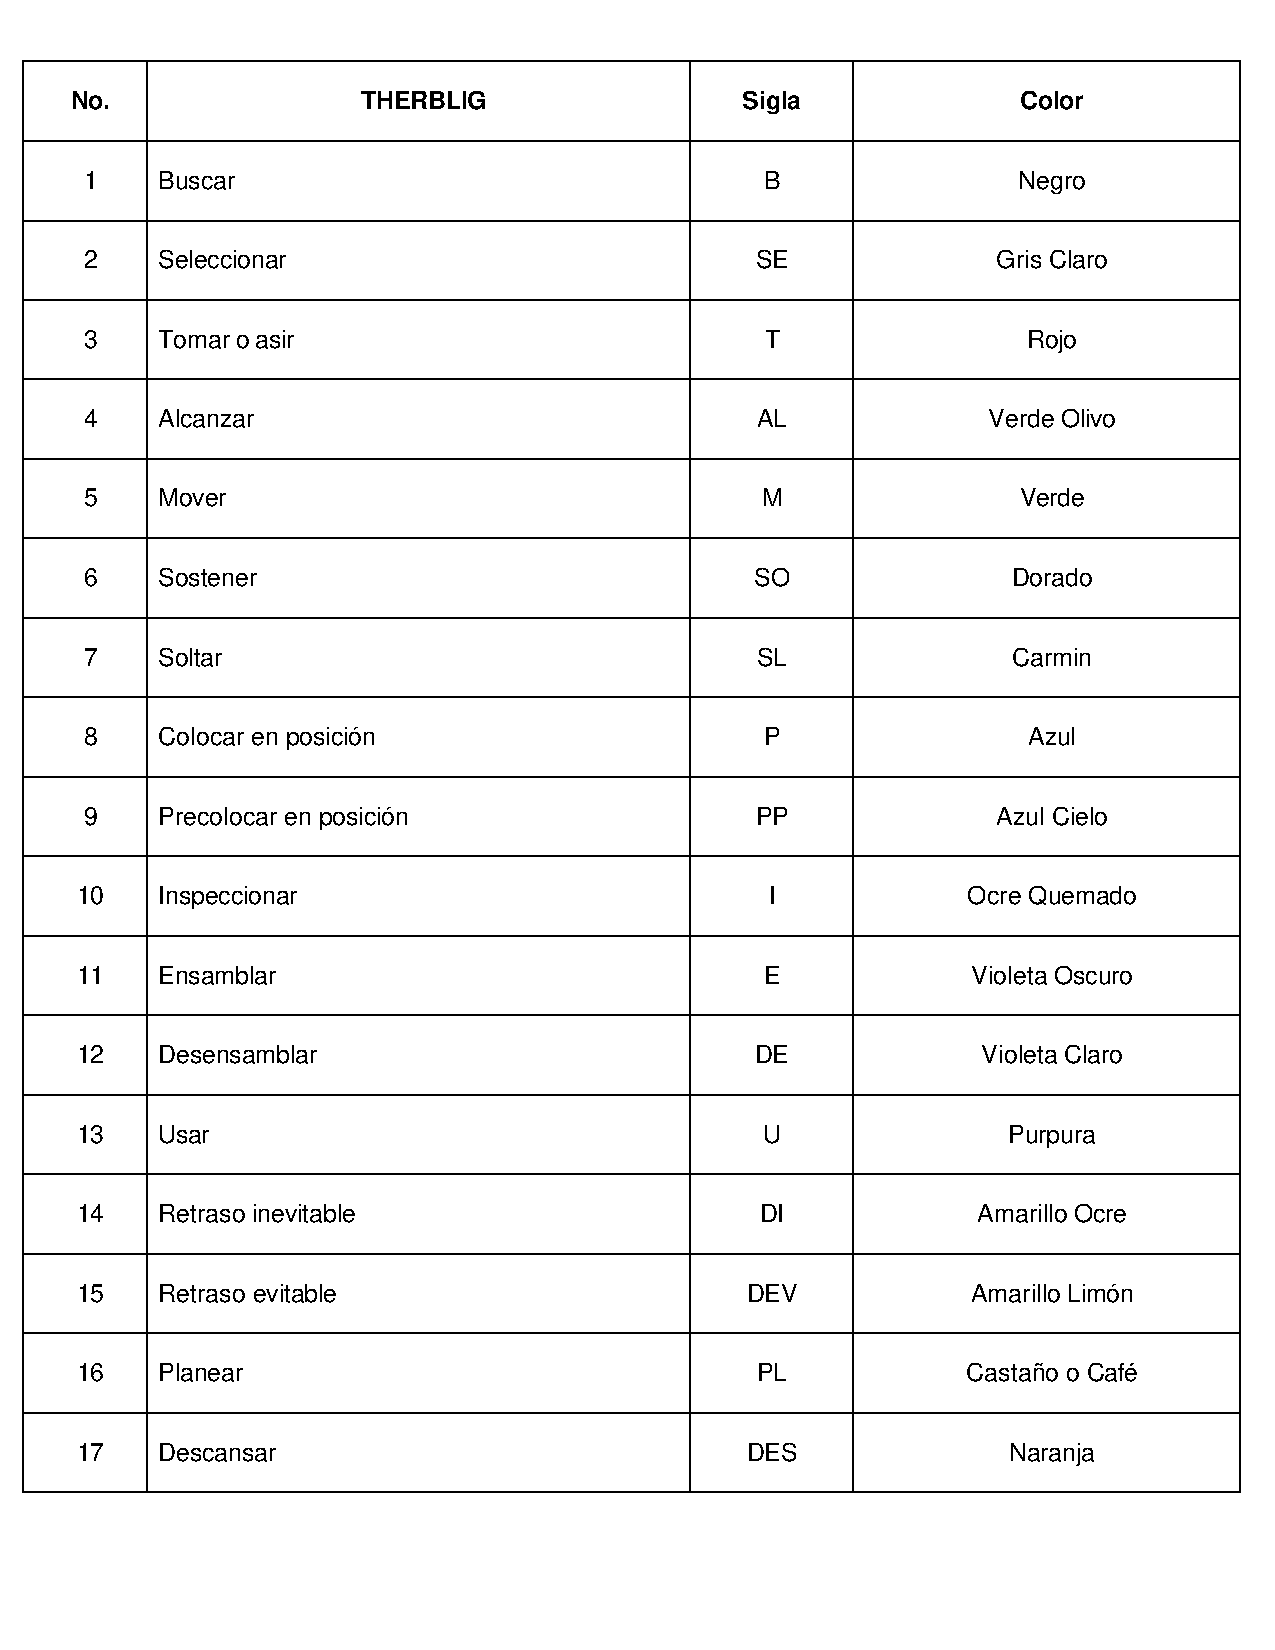
\includegraphics[scale=0.40]{13/img/tablaTherbling.pdf}
        \caption{17 therblings}
        \label{fig:therblings}
    \end{figure}
    Para realizar este sistema usamos de los therblings \ref{fig:therblings} los cuales nos ayudan a obtener nuestros tiempos.
    para obtener nuestros datos MTM utilizamos las siguientes tablas previamente echo el analices sobre los therblings.
    \begin{figure}[H]
        \centering
        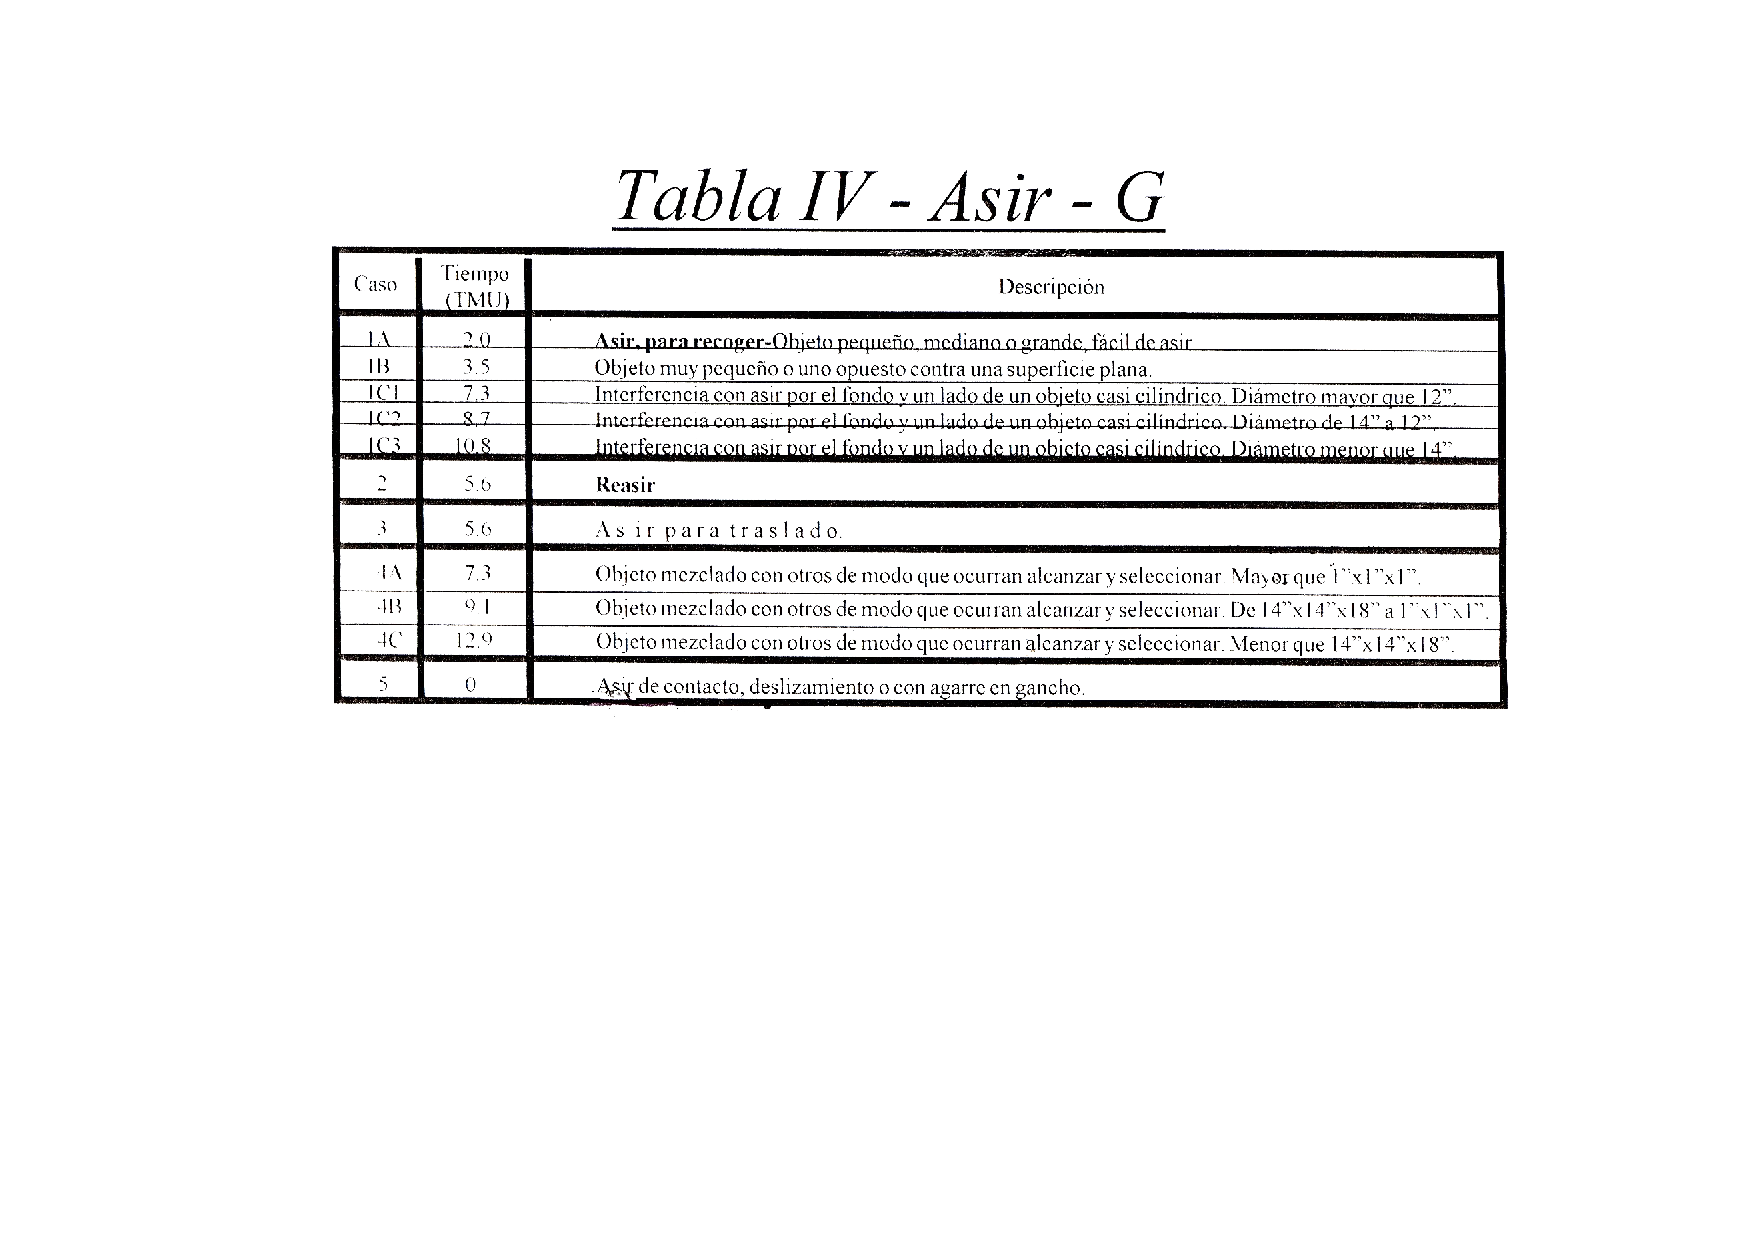
\includegraphics[scale=0.4]{13/img/tablaAsir.pdf}
        \caption{Asir}
        \label{fig:Asir}
    \end{figure}
    \begin{figure}[H]
        \centering
        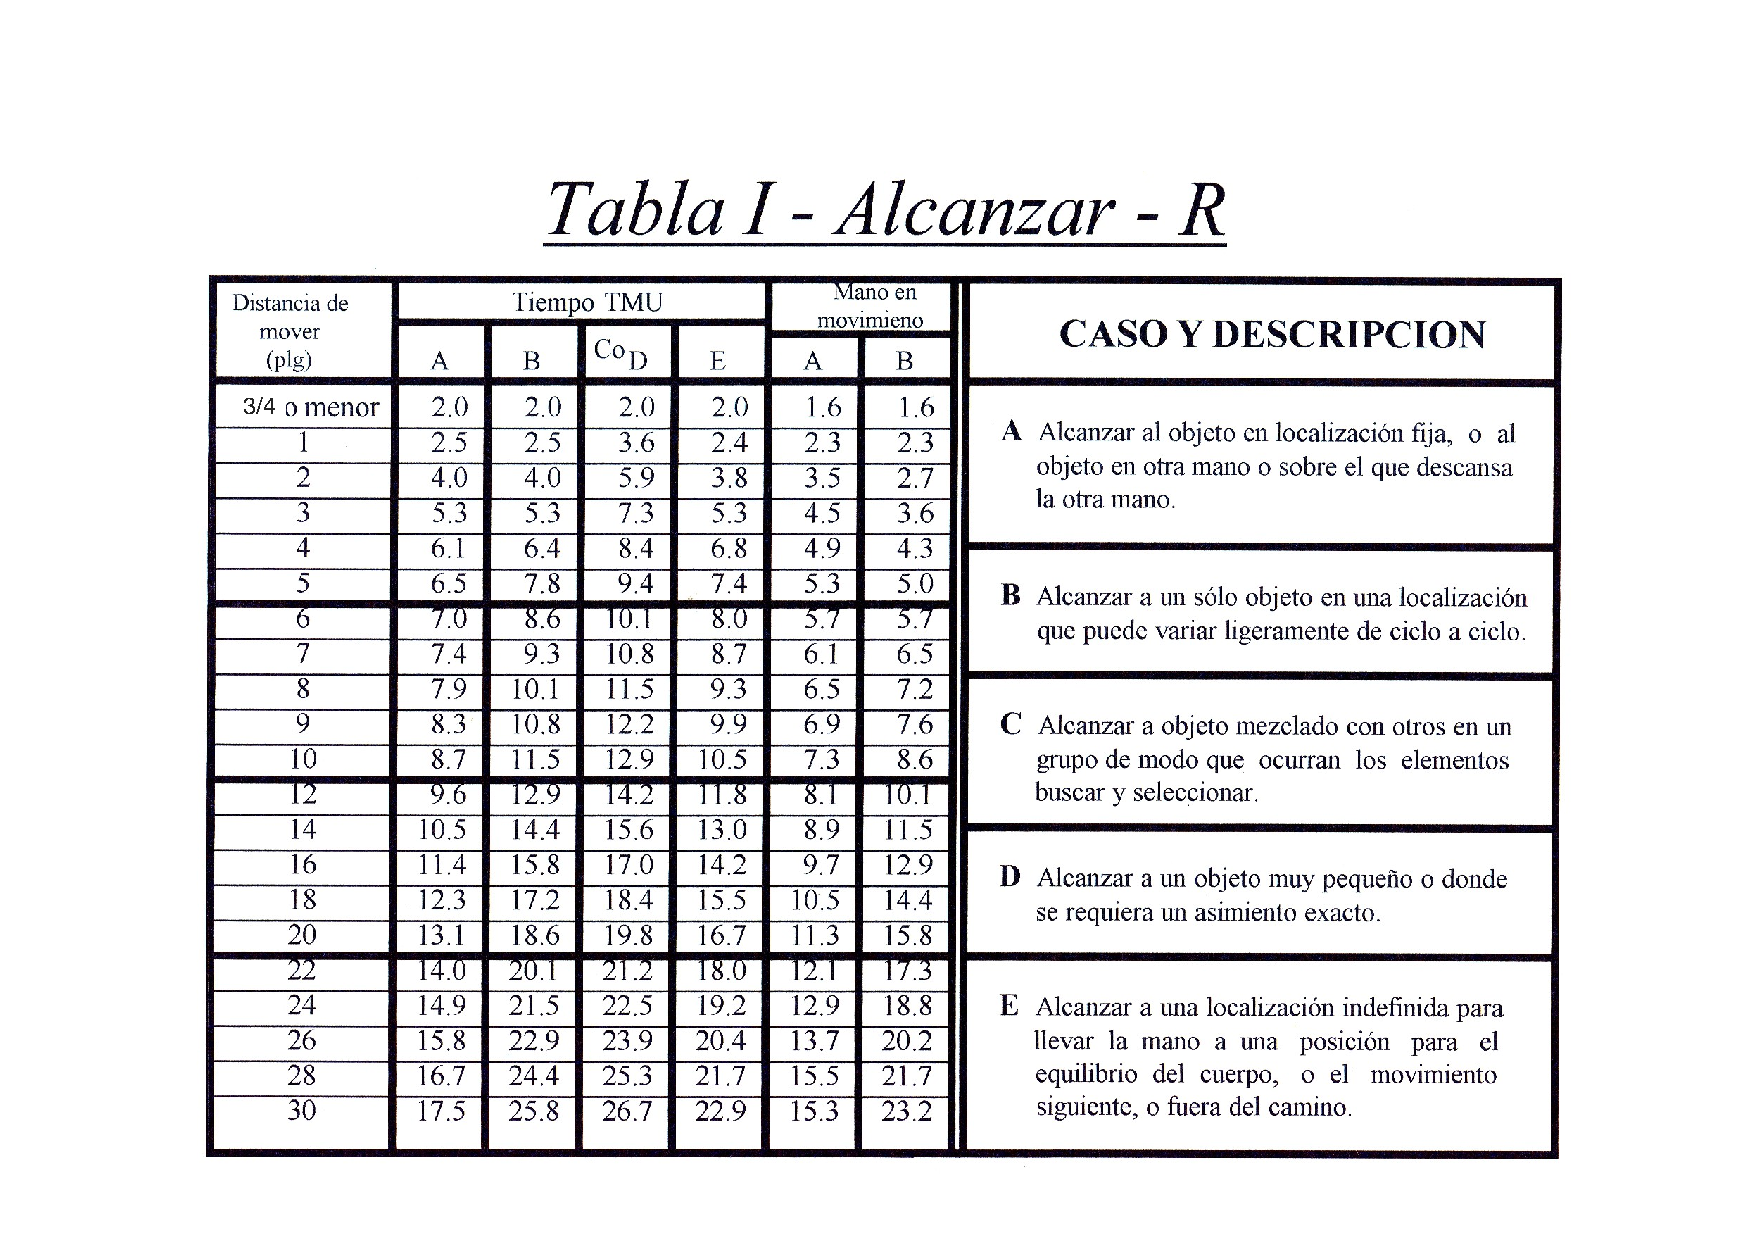
\includegraphics[scale=0.3]{13/img/tablaAlcanzar.pdf}
        \caption{Alcanzar}
        \label{fig:Alcanzar}
    \end{figure}
    \begin{figure}[H]
        \centering
        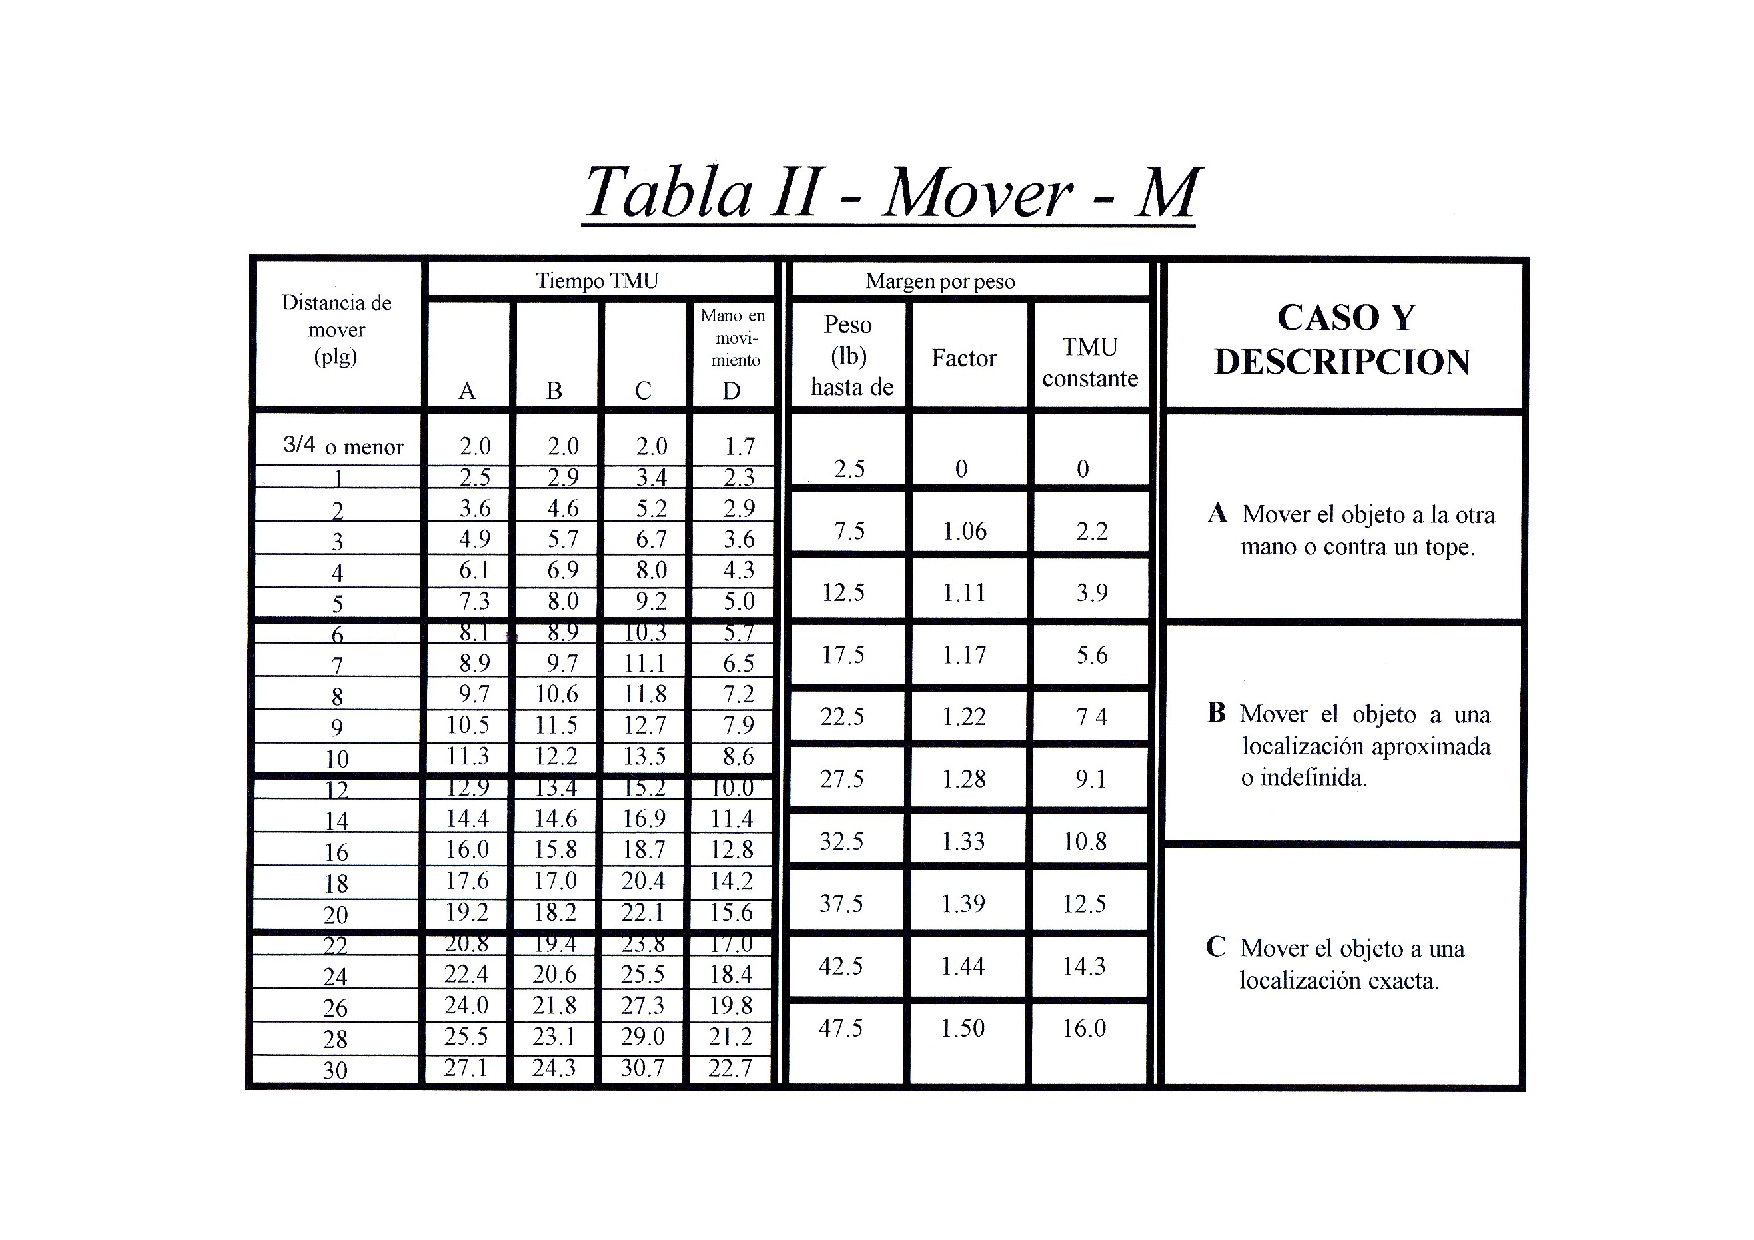
\includegraphics[scale=0.3]{13/img/tablaMover.pdf}
        \caption{Mover}
        \label{fig:Mover}
    \end{figure}
    \begin{figure}[H]
        \centering
        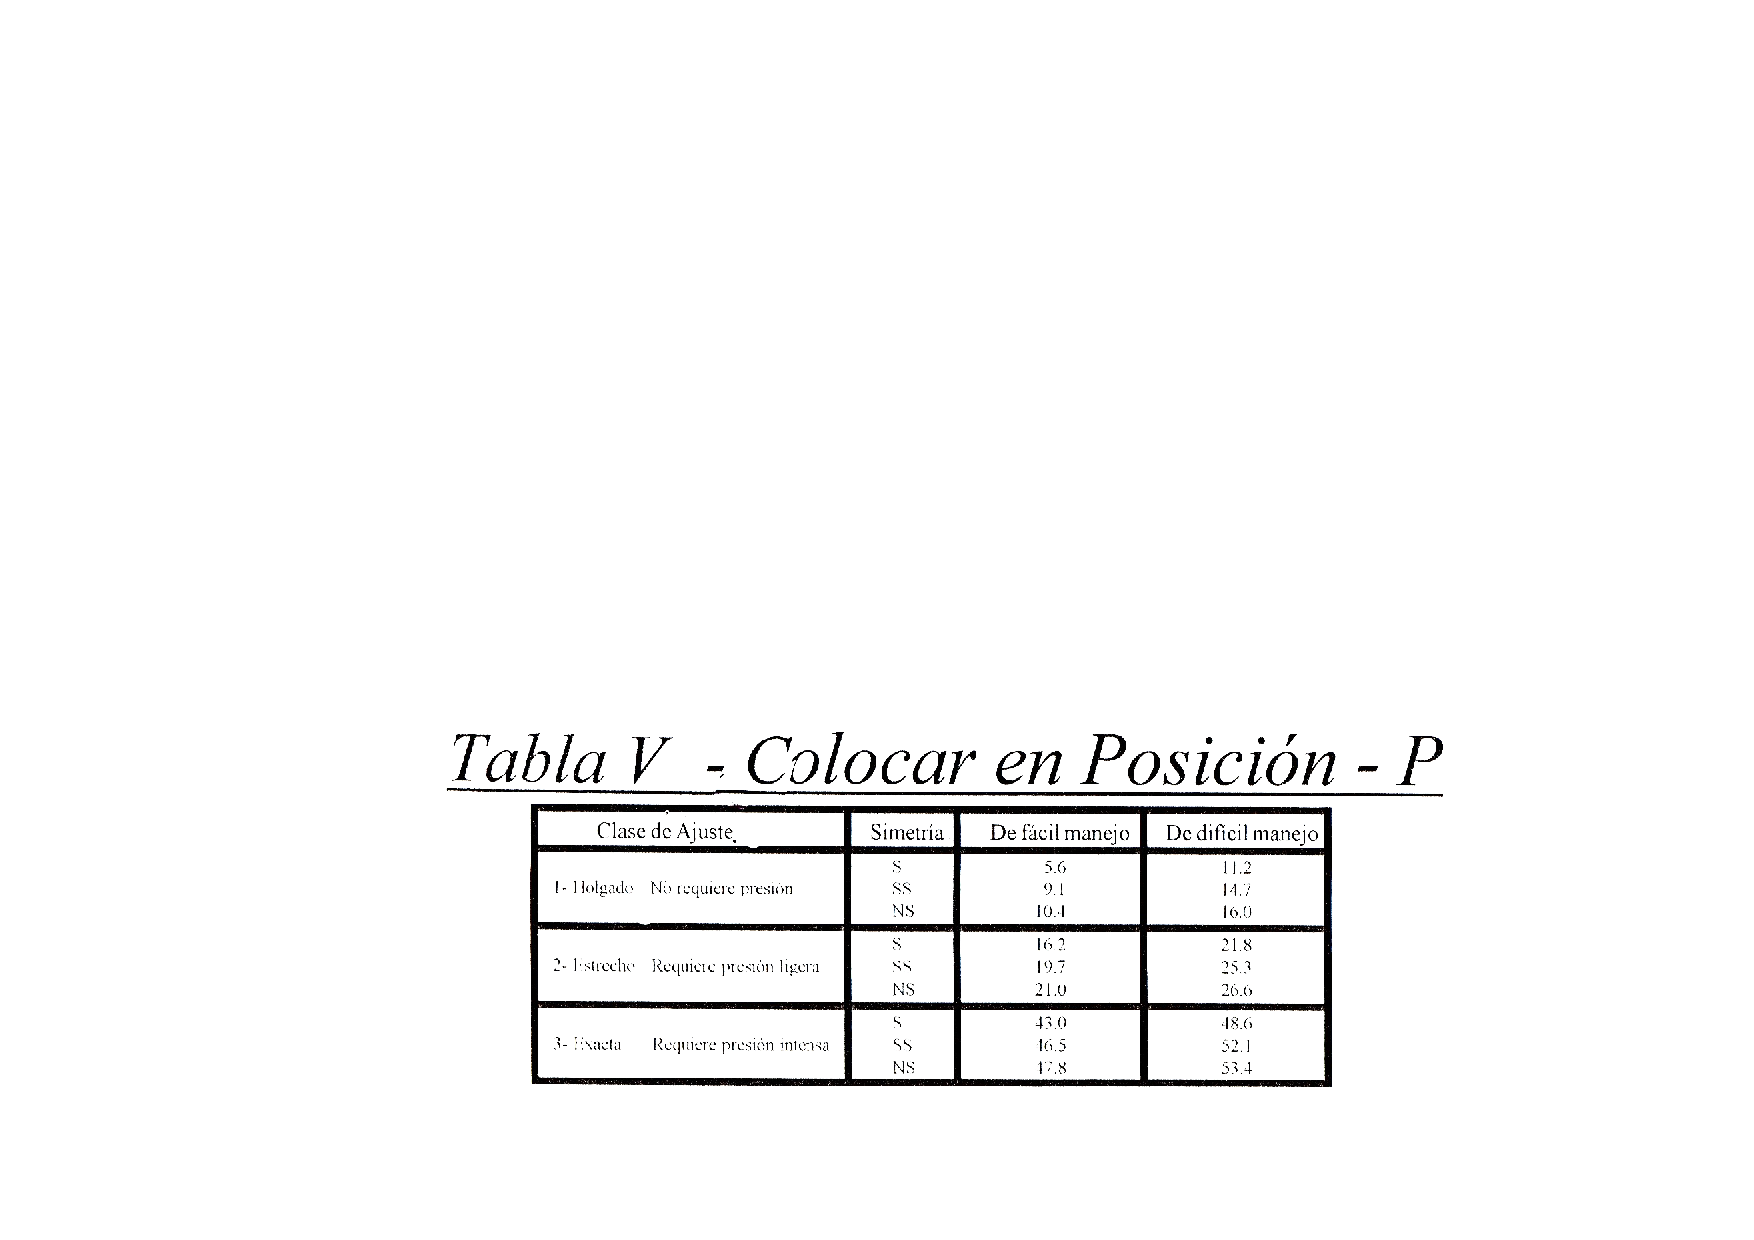
\includegraphics[scale=0.5]{13/img/tablaColocarPosicion.pdf}
        \caption{ColocarPosicion}
        \label{fig:ColocarPosicion}
    \end{figure}
    \begin{figure}[H]
        \centering
        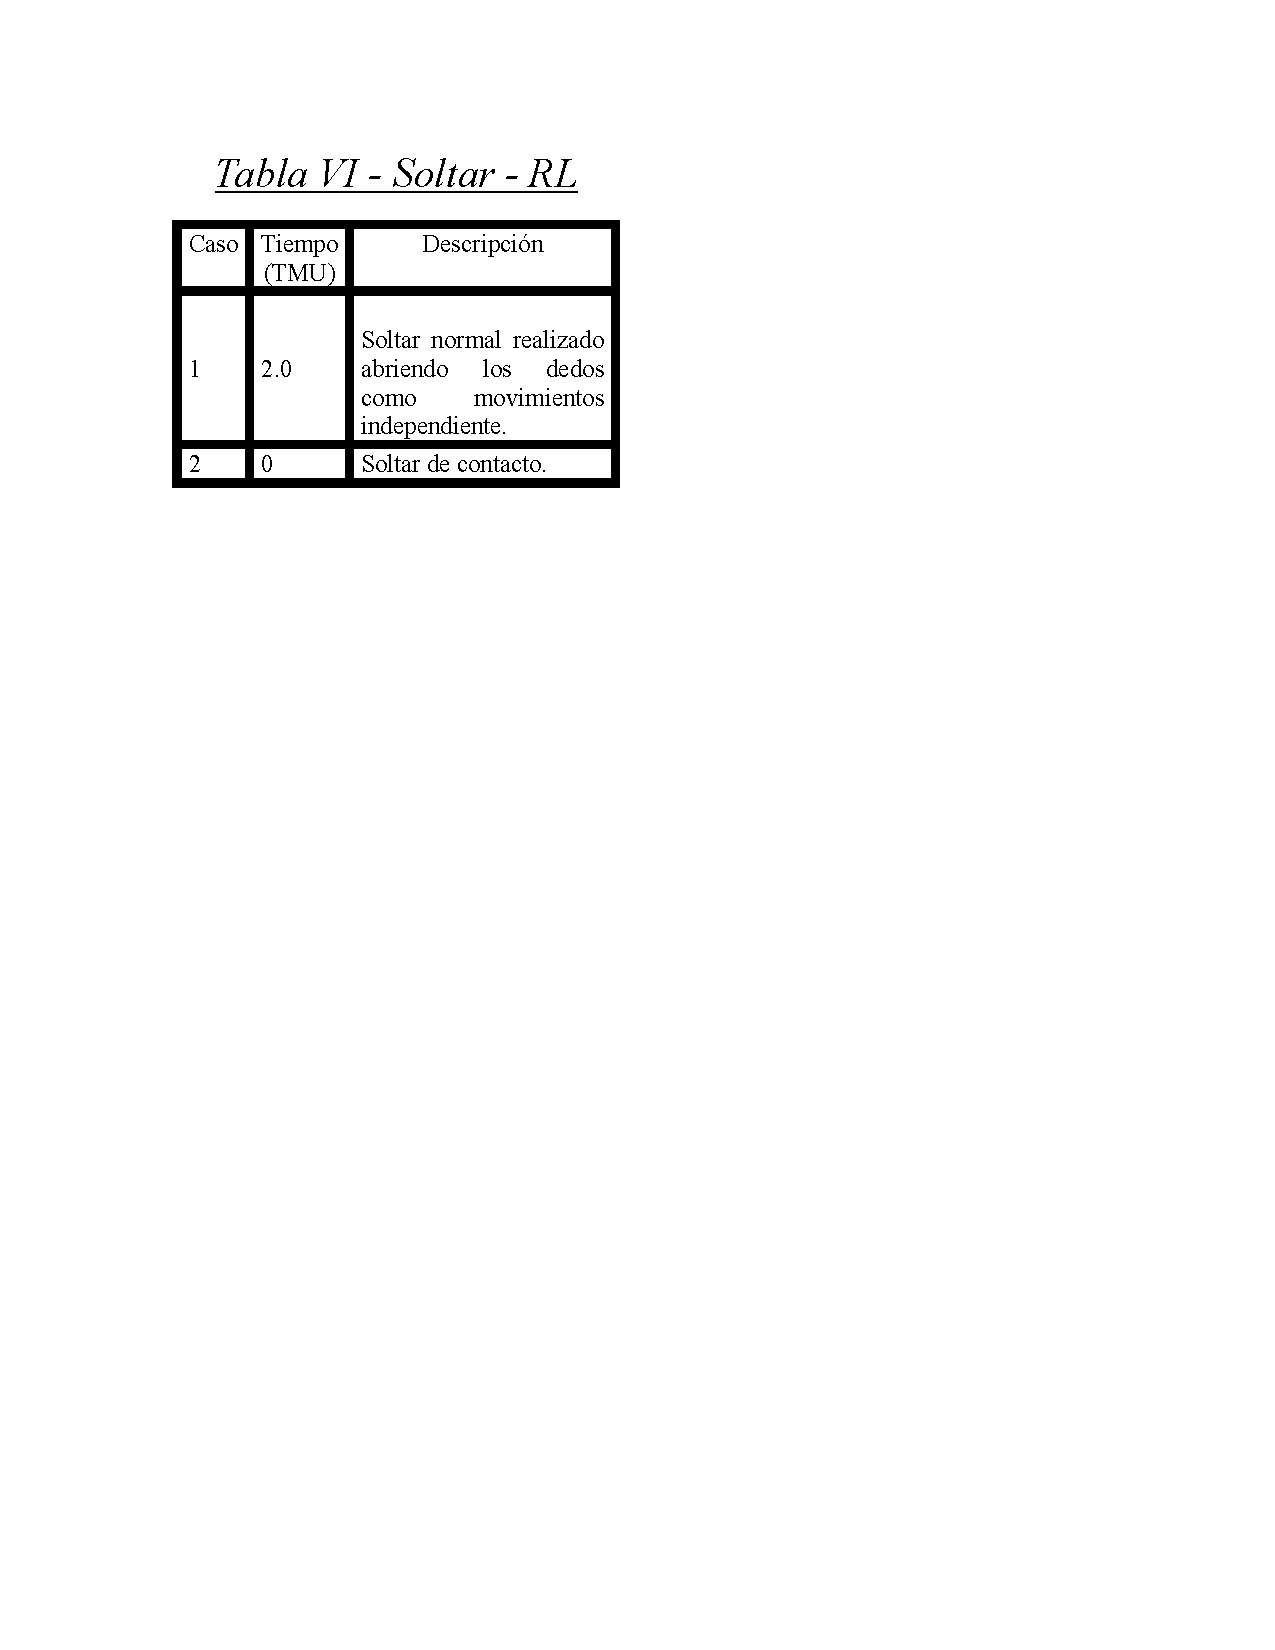
\includegraphics[scale=0.6]{13/img/tablaSoltar.pdf}
        \caption{Soltar}
        \label{fig:Soltar}
    \end{figure}
    % 
    \subsubsection{Desarrollo del muestreo del trabajo}
    % 
    En ingeniería industrial y gestión de operaciones, el muestreo del trabajo es una técnica para analizar la utilización del tiempo de trabajo y evaluar la eficiencia de los procesos. La técnica consiste en observar y documentar de manera casual lo que están haciendo los empleados o cómo se están utilizando las máquinas y otros recursos. De acuerdo con estas observaciones, es posible calcular la cantidad de tiempo destinado a diversas actividades, tanto las que son productivas como las que no lo son. El muestreo del trabajo se convierte en una herramienta esencial en los proyectos integradores para identificar ineficiencias, cuellos de botella y oportunidades de mejora.
    \begin{figure}[H]
        \centering
        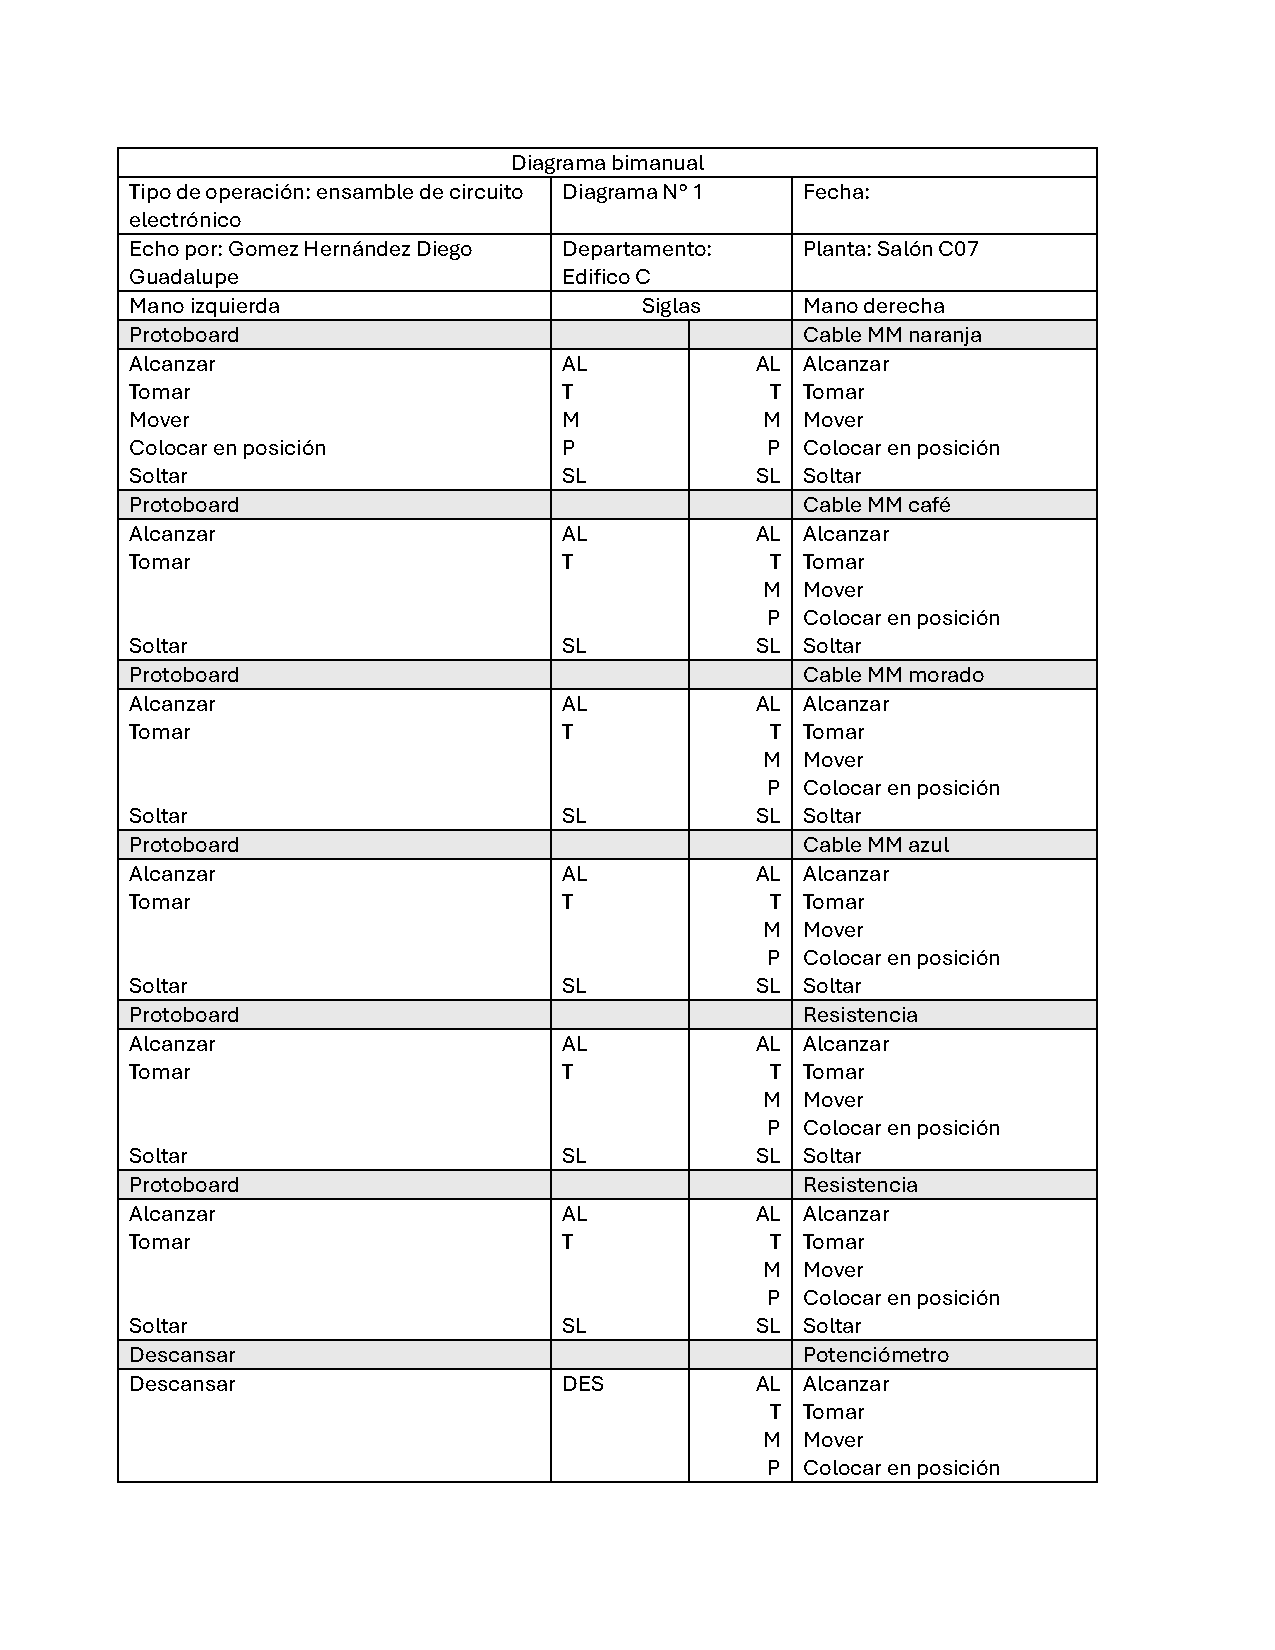
\includegraphics[scale=0.22]{13/img/diagramaBimanualUno.pdf}
        \centering
        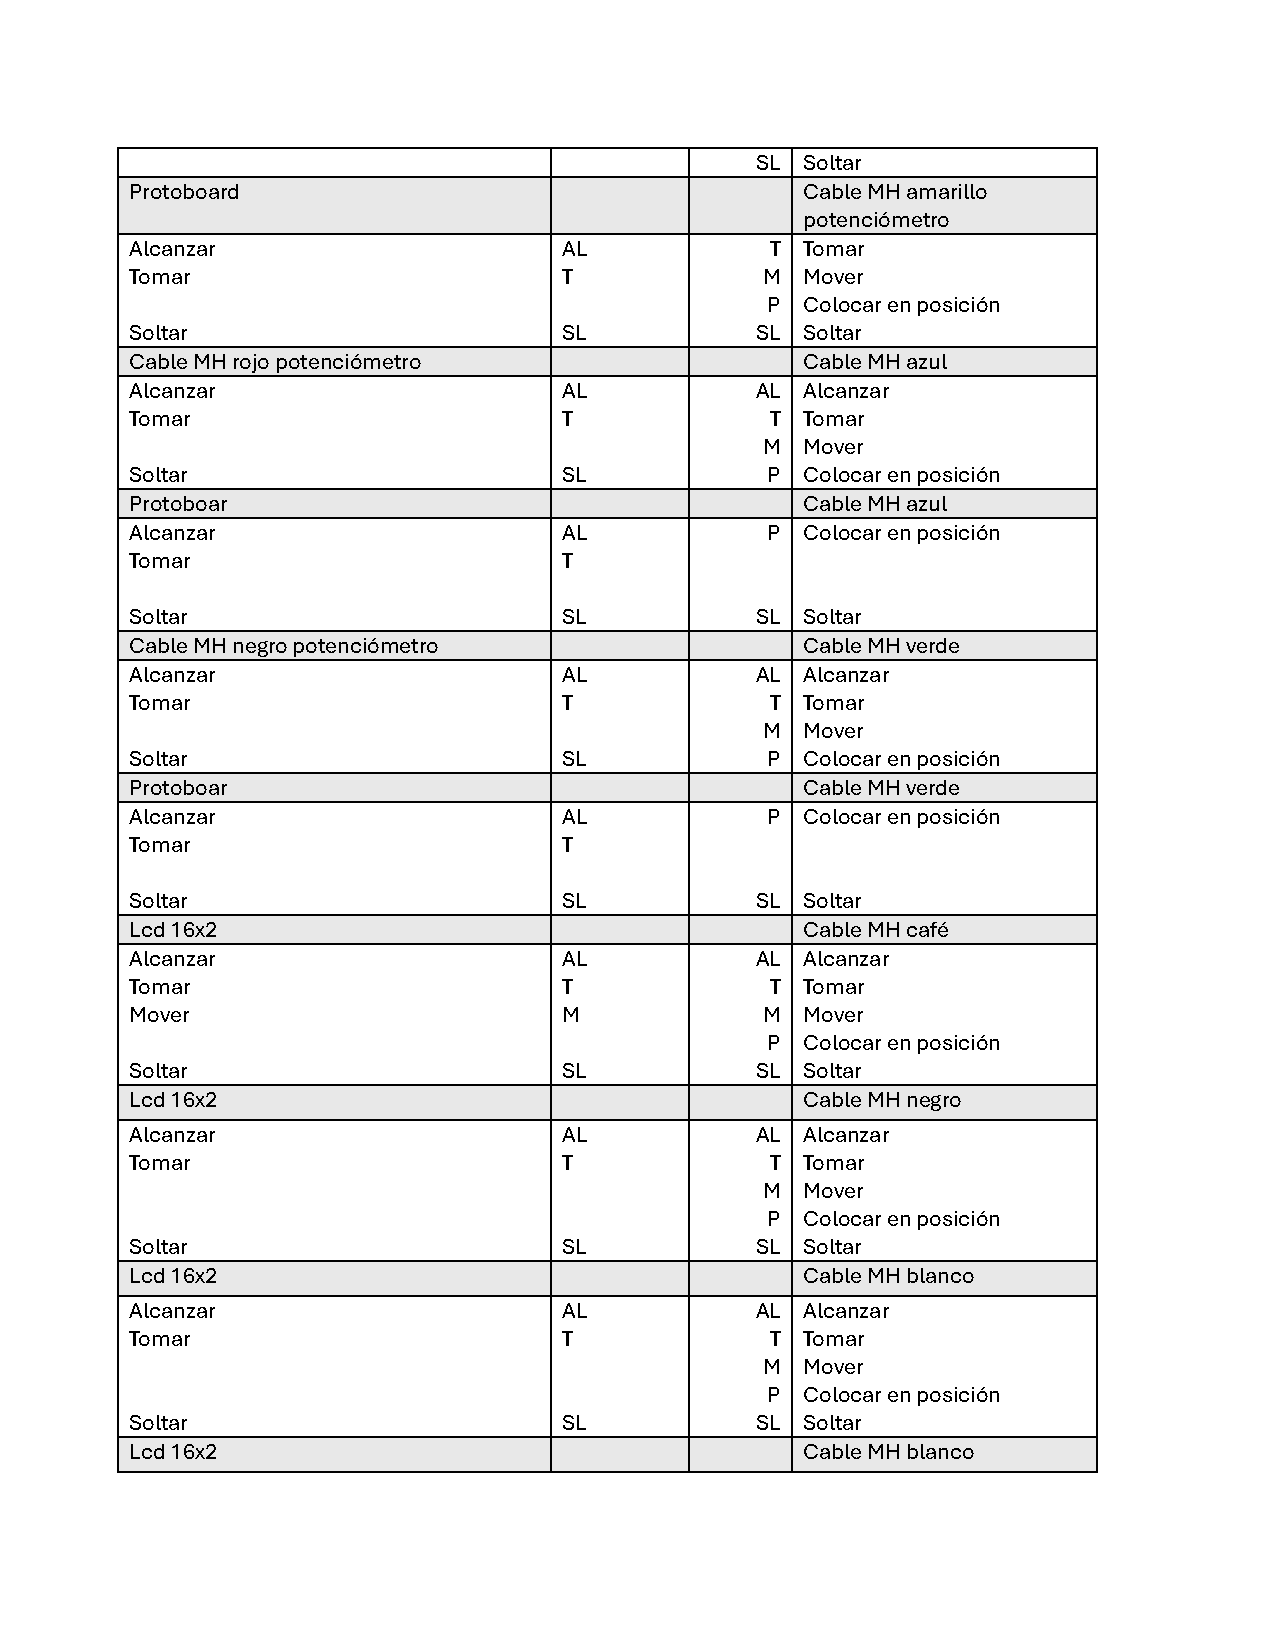
\includegraphics[scale=0.22]{13/img/diagramaBimanualDos.pdf}
        \centering
        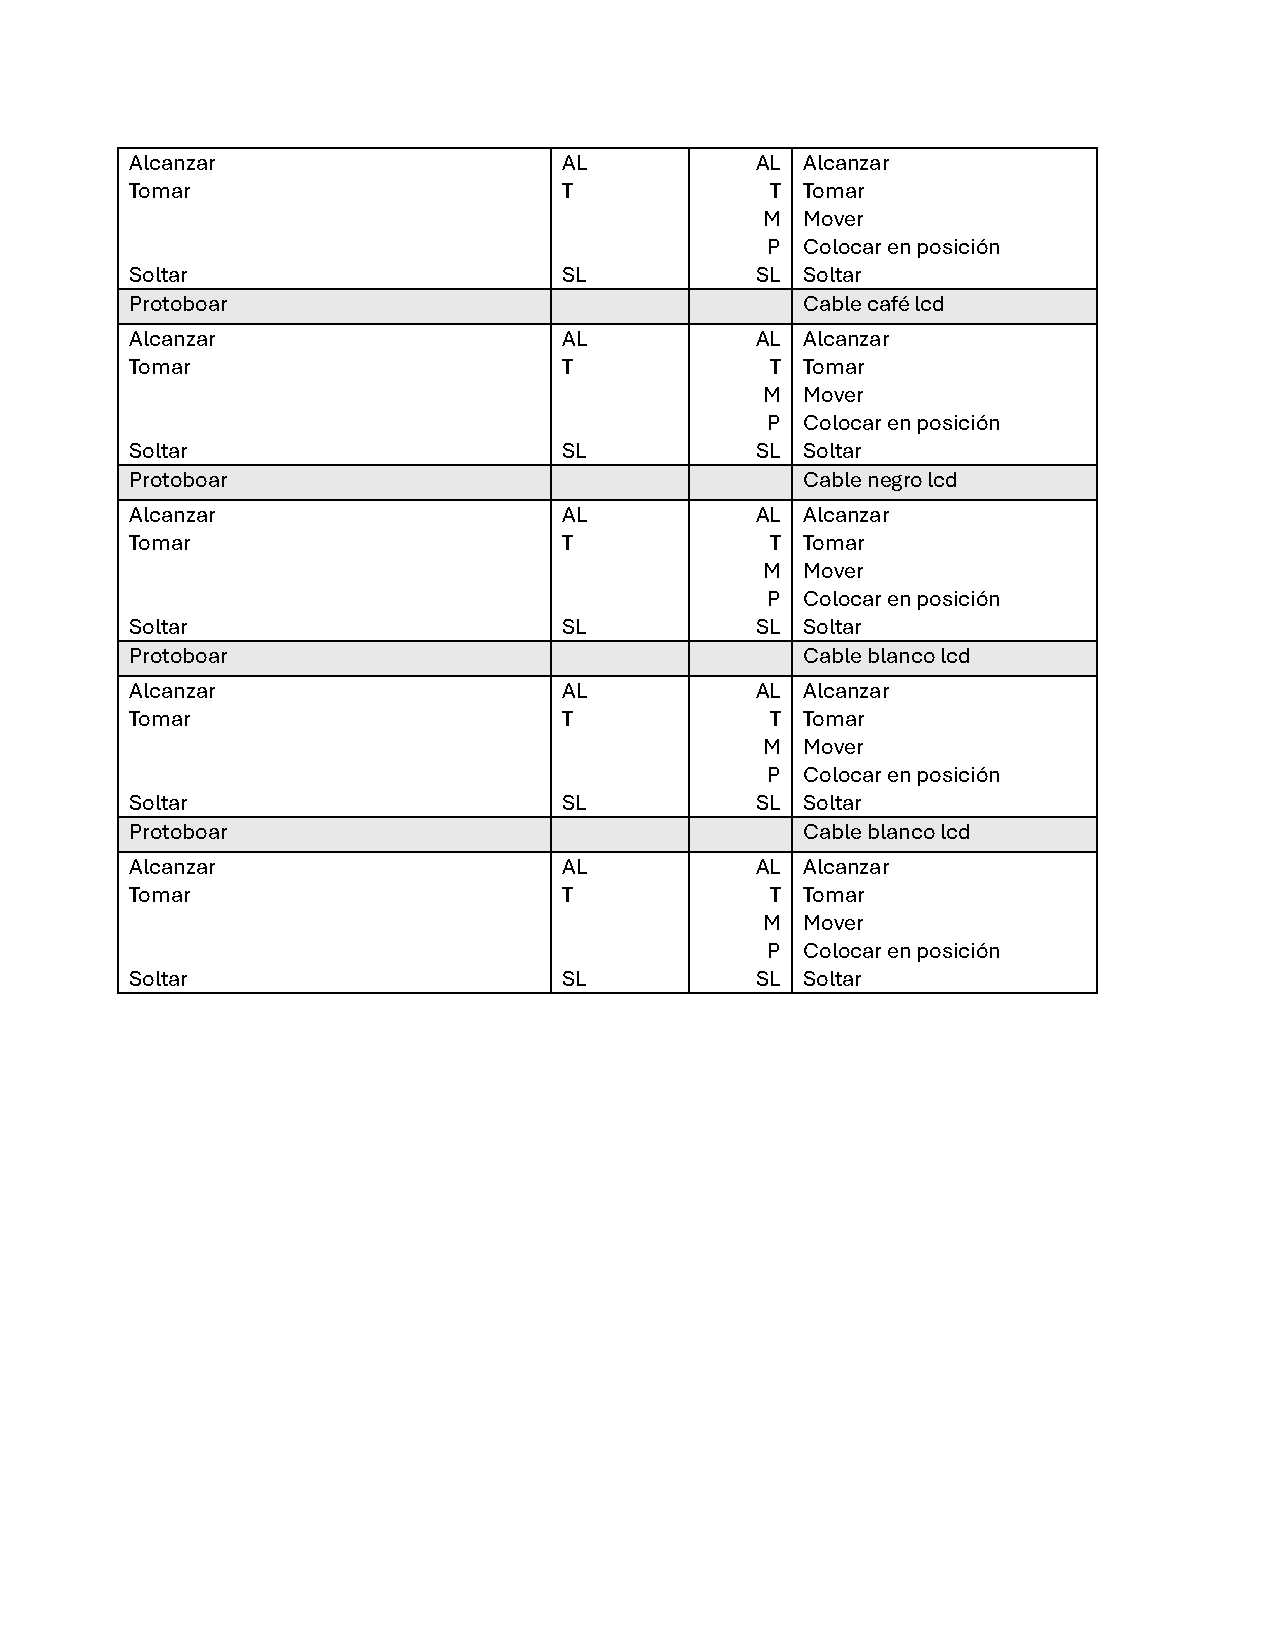
\includegraphics[scale=0.22]{13/img/diagramaBimanualTres.pdf}
        \caption{diagrama Bimanual}
        \label{fig:diagramaBimanual}
    \end{figure}
    % 
    \subsubsection{Corrección por balanceo de procesos}
    % 
    Para optimizar la distribución de trabajo a lo largo de una línea de producción o ensamblaje, se utiliza la corrección por balanceo de procesos en gestión de operaciones e ingeniería industrial. El balanceo de procesos tiene como objetivo principal reducir los tiempos de inactividad y desequilibrios entre las estaciones de trabajo, garantizando que cada estación tenga una carga de trabajo equilibrada y que el flujo de producción sea lo más continuo y eficiente posible. El uso del balanceo de procesos en proyectos integradores es fundamental para aumentar la eficiencia y la productividad.
    % 
    \subsubsection{Datos estándar continuos y discretos}
    % 
    % 
    Datos Estándar Continuos: Estos datos se expresan en unidades de tiempo continuas, como minutos o segundos. Se utilizan para medir tareas que fluyen continuamente y son difíciles de dividir en partes discretas. Por ejemplo, el tiempo que lleva ensamblar un componente electrónico puede medirse en minutos o segundos.
    
    Datos Estándar Discretos: Estos datos muestran el tiempo en unidades discretas, como movimientos individuales o unidades de trabajo. Se utilizan para medir tareas que se pueden dividir en pasos o movimientos individuales. Por ejemplo, se pueden usar unidades discretas para medir el tiempo que lleva conectar un cable a un ensamble electrónico.
    
    Ambos tipos de datos son cruciales para comprender y optimizar los procesos de producción. Los datos discretos permiten un análisis más detallado de las tareas individuales, mientras que los datos continuos brindan una visión completa del flujo de trabajo. La combinación de ambos tipos de datos puede facilitar la identificación de áreas de mejora y optimización en procesos productivos como el ensamblaje electrónico.
    % 
    % 
    
    % 
    % 
    \subsection{Diseño de la forma más económica de realizar el trabajo}
    % 
    El enfoque de diseño de la forma más económica de realizar el trabajo se centra en encontrar la manera más eficiente y rentable de realizar las tareas necesarias para completar un proceso o proyecto. Esto implica la identificación y el uso de técnicas, materiales y recursos que reduzcan los costos sin sacrificar la calidad del resultado final. Dicho diseño es crucial para maximizar la eficiencia y reducir los costos de construcción de circuitos electrónicos.
    
    Para lograrlo, es esencial examinar minuciosamente cada paso del proceso de ensamblaje para encontrar oportunidades de optimización en términos de costos de materiales y recursos utilizados. Esto incluye el análisis del flujo de trabajo, el tiempo requerido para cada tarea, los recursos humanos y tecnológicos involucrados y los materiales utilizados. Se pueden reducir los costos totales y aumentar la rentabilidad del proceso de producción al hacer mejoras en estos aspectos sin sacrificar la calidad y la funcionalidad del producto final.
    
    Este método completo no solo reduce los costos, sino que también mejora la sostenibilidad y la competitividad del proceso de producción de circuitos electrónicos.
    % 
    \subsection{Normalización de los métodos, materiales, herramientas e instalaciones}
    % 
    La estandarización de métodos, materiales, herramientas e instalaciones es esencial para este proyecto porque garantiza la calidad, la seguridad y la eficiencia del ensamblaje de circuitos electrónicos. Los estándares uniformes aseguran la compatibilidad de los componentes y reducen los costos al reducir la cantidad de errores y retrabajos. Además, proporciona pautas claras para el uso de herramientas y la selección de materiales, mejorando la consistencia y la confiabilidad del proyecto. La innovación se fomenta al cumplir con estas normas, lo que facilita la integración de nuevas tecnologías en el diseño y fabricación de circuitos.
    
    Los materiales que usaremos fueron elegidos para poder obtener datos claros y poder llevar a cabo nuestra obtención de datos sin ninguna interferencia. los materiales a elegir se mostraran en la siguiente tabla.\ref{fig:materiales}
    \begin{figure}[H]
        \centering
        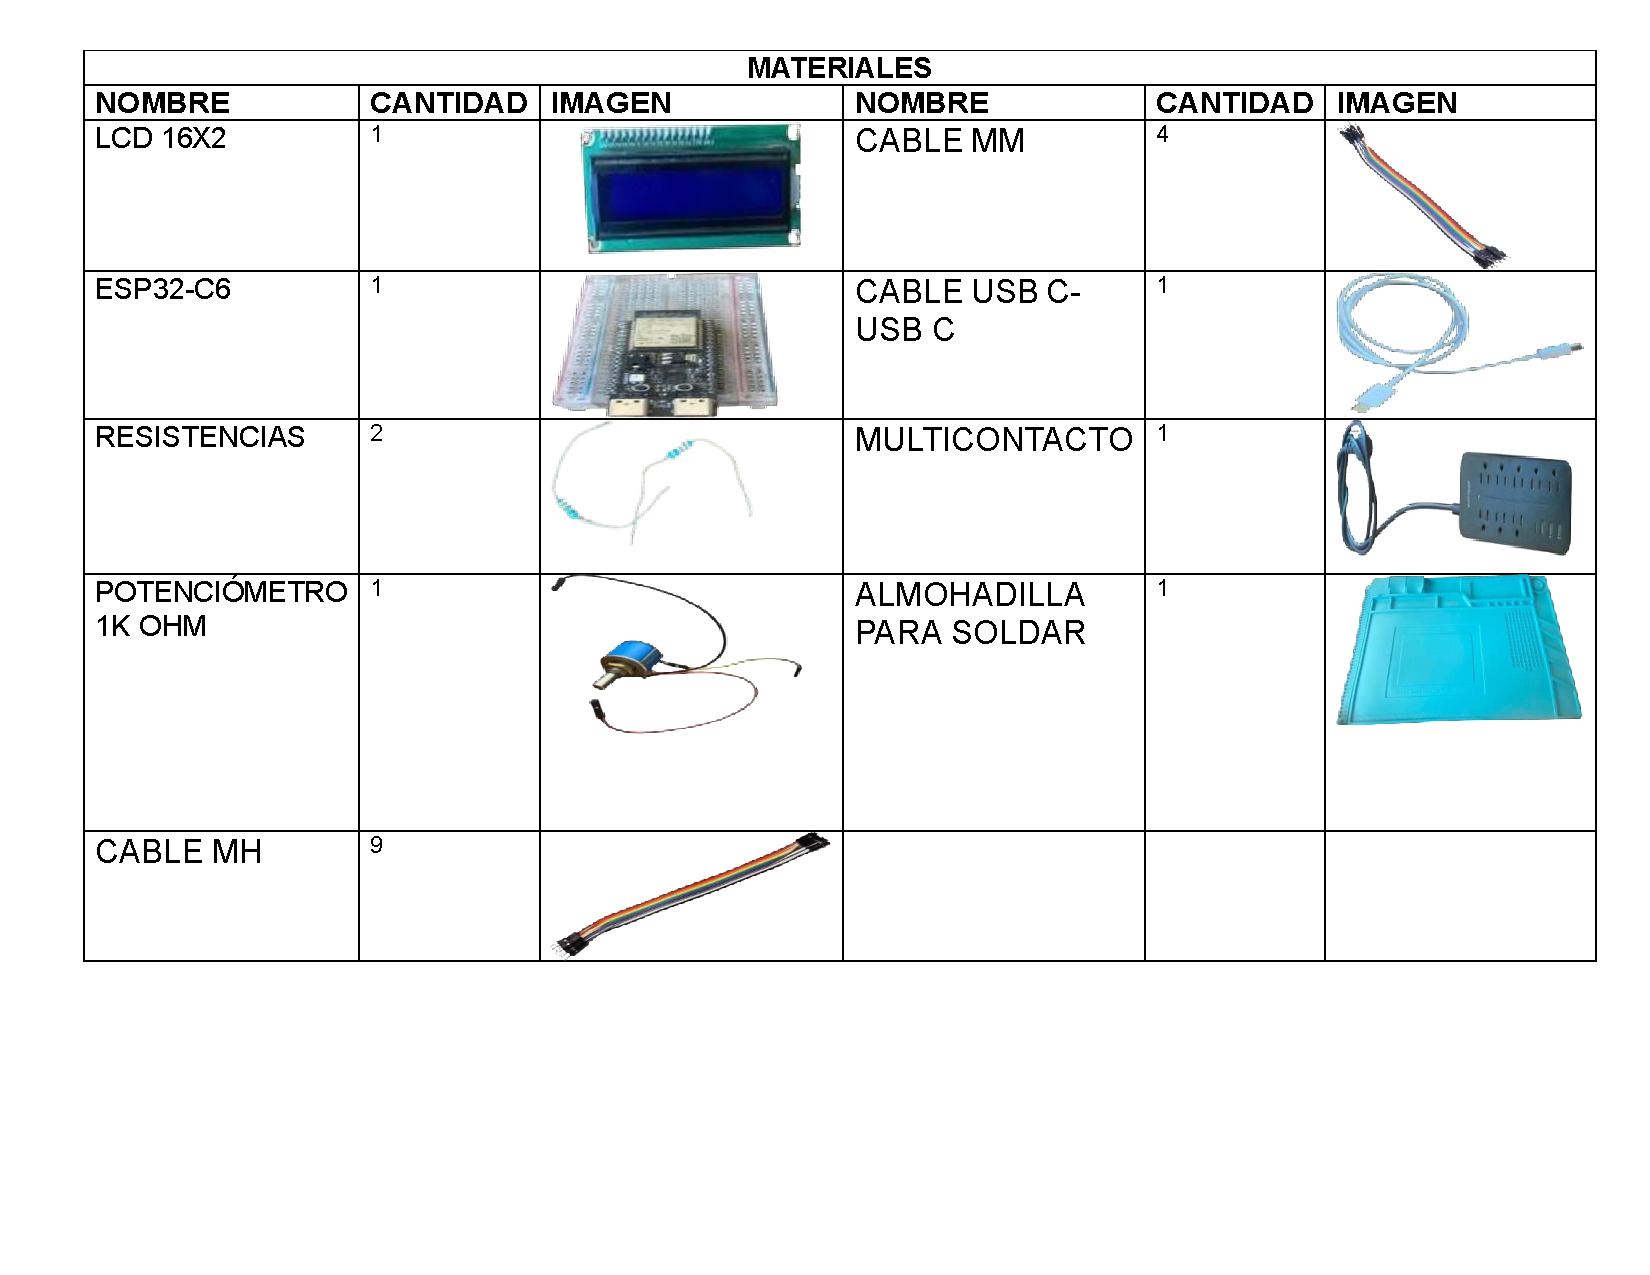
\includegraphics[scale=0.30]{13/img/materiales.pdf}
        \caption{materiales}
        \label{fig:materiales}
    \end{figure}
    % 
    \subsection{Determinación del tiempo estándar para que una persona competente realice el trabajo con marcha normal}
    
    % 
    % 
    % \subsection{Acrónimos y Abreviaciones}
    
    % Los acrónimos y abreviaciones deberán ser definidos únicamente la primera vez que aparecen en el texto, esto para que el lector entienda lo que significan.
    
    % \subsection{Ecuaciones}
    
    % Las ecuaciones son una excepción a las especificaciones prescritas de esta plantilla. 
    % Deberá determinar si su ecuación debe escribirse o no utilizando la fuente Adobe Devangari. 
    % Para crear ecuaciones multinivel, puede ser necesario tratar la ecuación como un gráfico e insertarla en el texto después de aplicar el estilo de la platilla.
    % Las ecuaciones serán enumeradas de manera consecutiva, y el número de ecuación, entre paréntesis, se colocan al ras de la derecha, utilizando una tabulación derecha.
    % 
    % \begin{equation}
    %     \label{eq1}
    %     x + y = z 
    % \end{equation}
    % 
    % Es importante asegurarse de que los símbolos de la ecuación sean definidos antes o inmediatamente después de la ecuación. Utilice “(1)”, en vez de “Eq. 1” al enumerar las ecuaciones, excepto al principio de una oración: “La ecuación (\ref{eq1}) es…”
    
    \section{Resultados y discusión}
    
    \subsection{Desarrollo de la guía de plan de Emergencia}
    
    Al realizar la guía de plan de emergencia estaremos previniendo riesgos de incendio, riesgos de daños físicos y evitando accidentes en el Instituto Tecnológico de Querétaro, capacitando al personal y teniendo un registro de estos mismos podremos contar con personal capacitado para para salvaguardar la integridad física y que estos tomen las mejores decisiones a la hora de actuar.
    Los datos del Instituto Tecnológico de Querétaro se resumen en la figura  \ref{fig:croquisTec}.
    % 
    % 
    \begin{figure}[H]
        \centering
        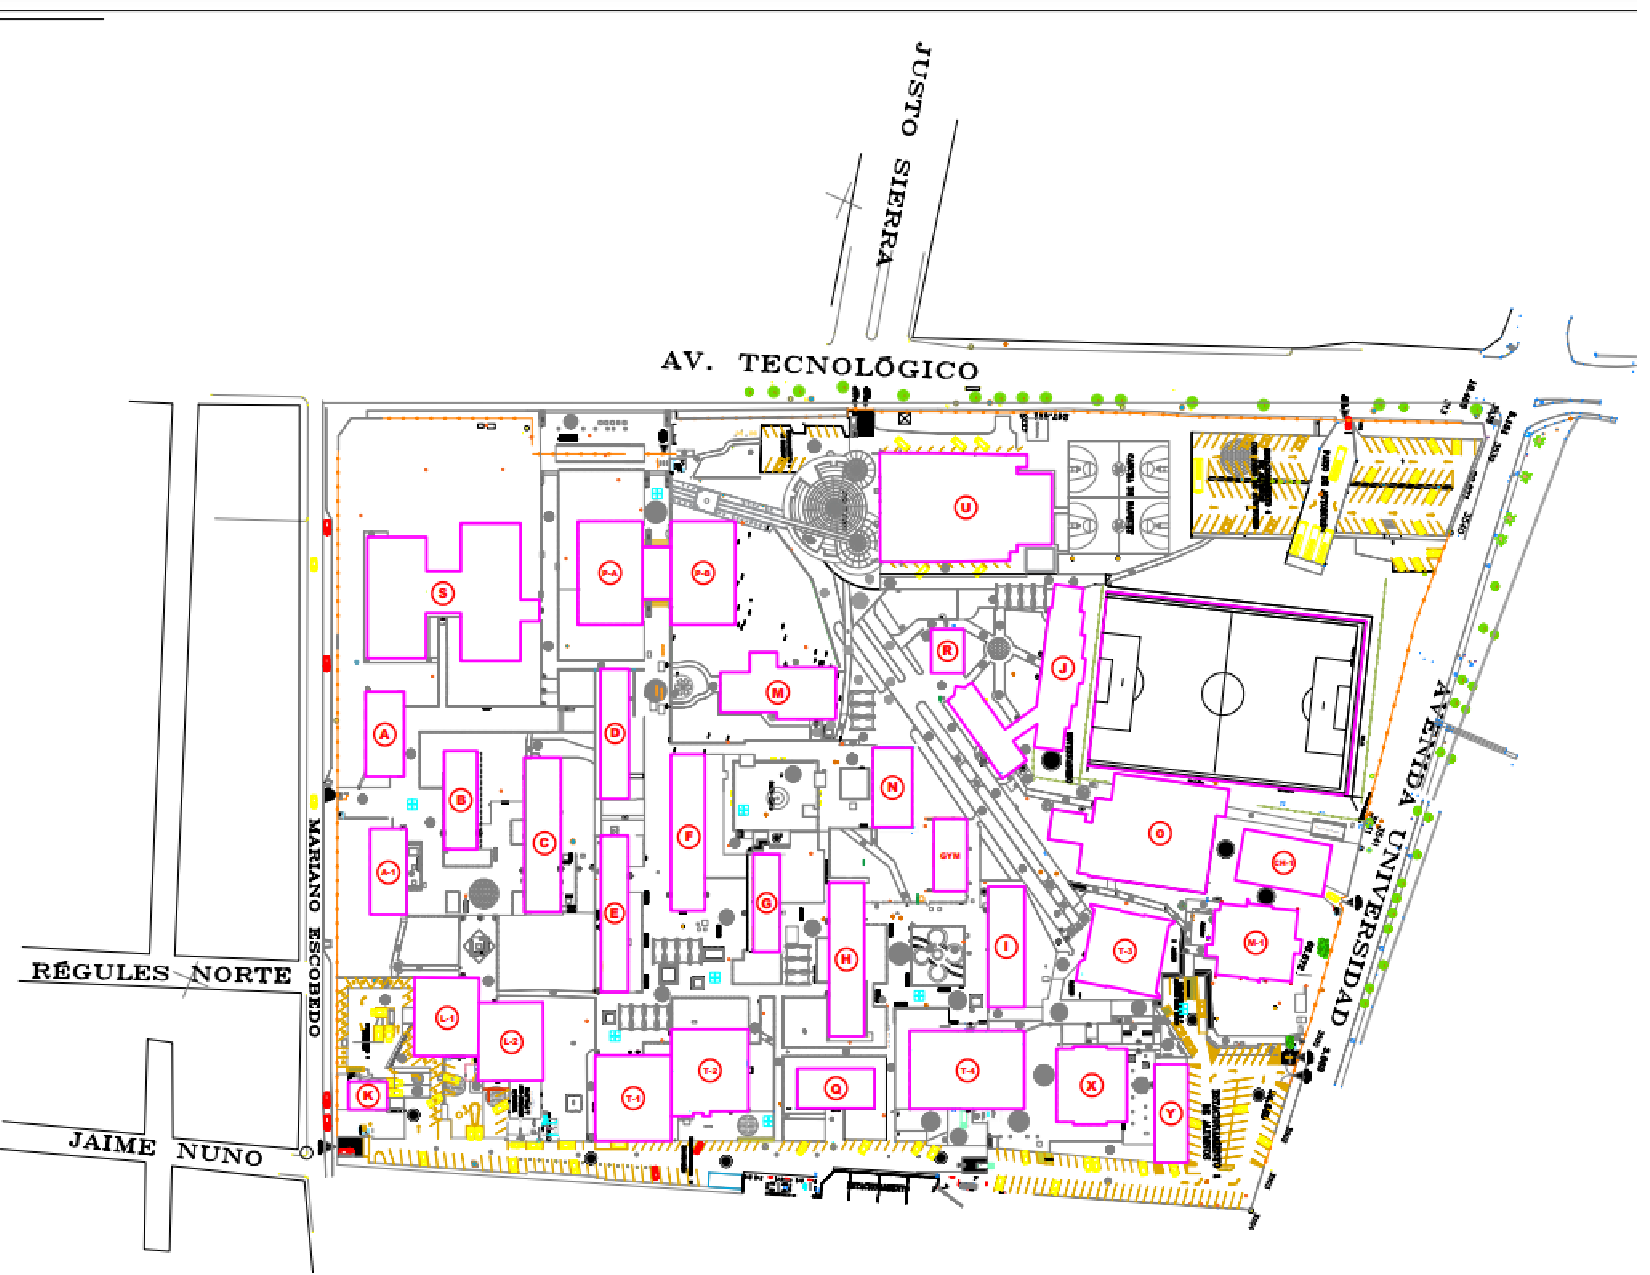
\includegraphics[scale=0.3]{13/img/croquisTec.pdf}
        \caption{Tecnológico Nacional de México, Instituto Tecnológico de Querétaro, Av Tecnológico S/N, Centro Histórico, Centro, 76000, Querétaro, Qro., 4422274400 Ext. 4423}
        \label{fig:croquisTec}
    \end{figure}
    % 
    % 
    \subsubsection{Identificación del riesgo}
    
    llevaremos a cabo un programa de prevención de riesgos interno y externo todos los días, así como a solicitar comentarios de clientes internos y externos sobre los riesgos presentes en nuestras actividades diarias. Invitando al equipo de trabajo a participar activamente en este proceso.
    Cada riesgo interno y externo se clasificará y evaluará según su importancia, lo que nos permitirá priorizar nuestras acciones y tomar las medidas adecuadas para abordarlos.En la siguiente imagen podremos ver la tabla de riesgos.
    % 
    % 
    \begin{figure}[H]
        \centering
        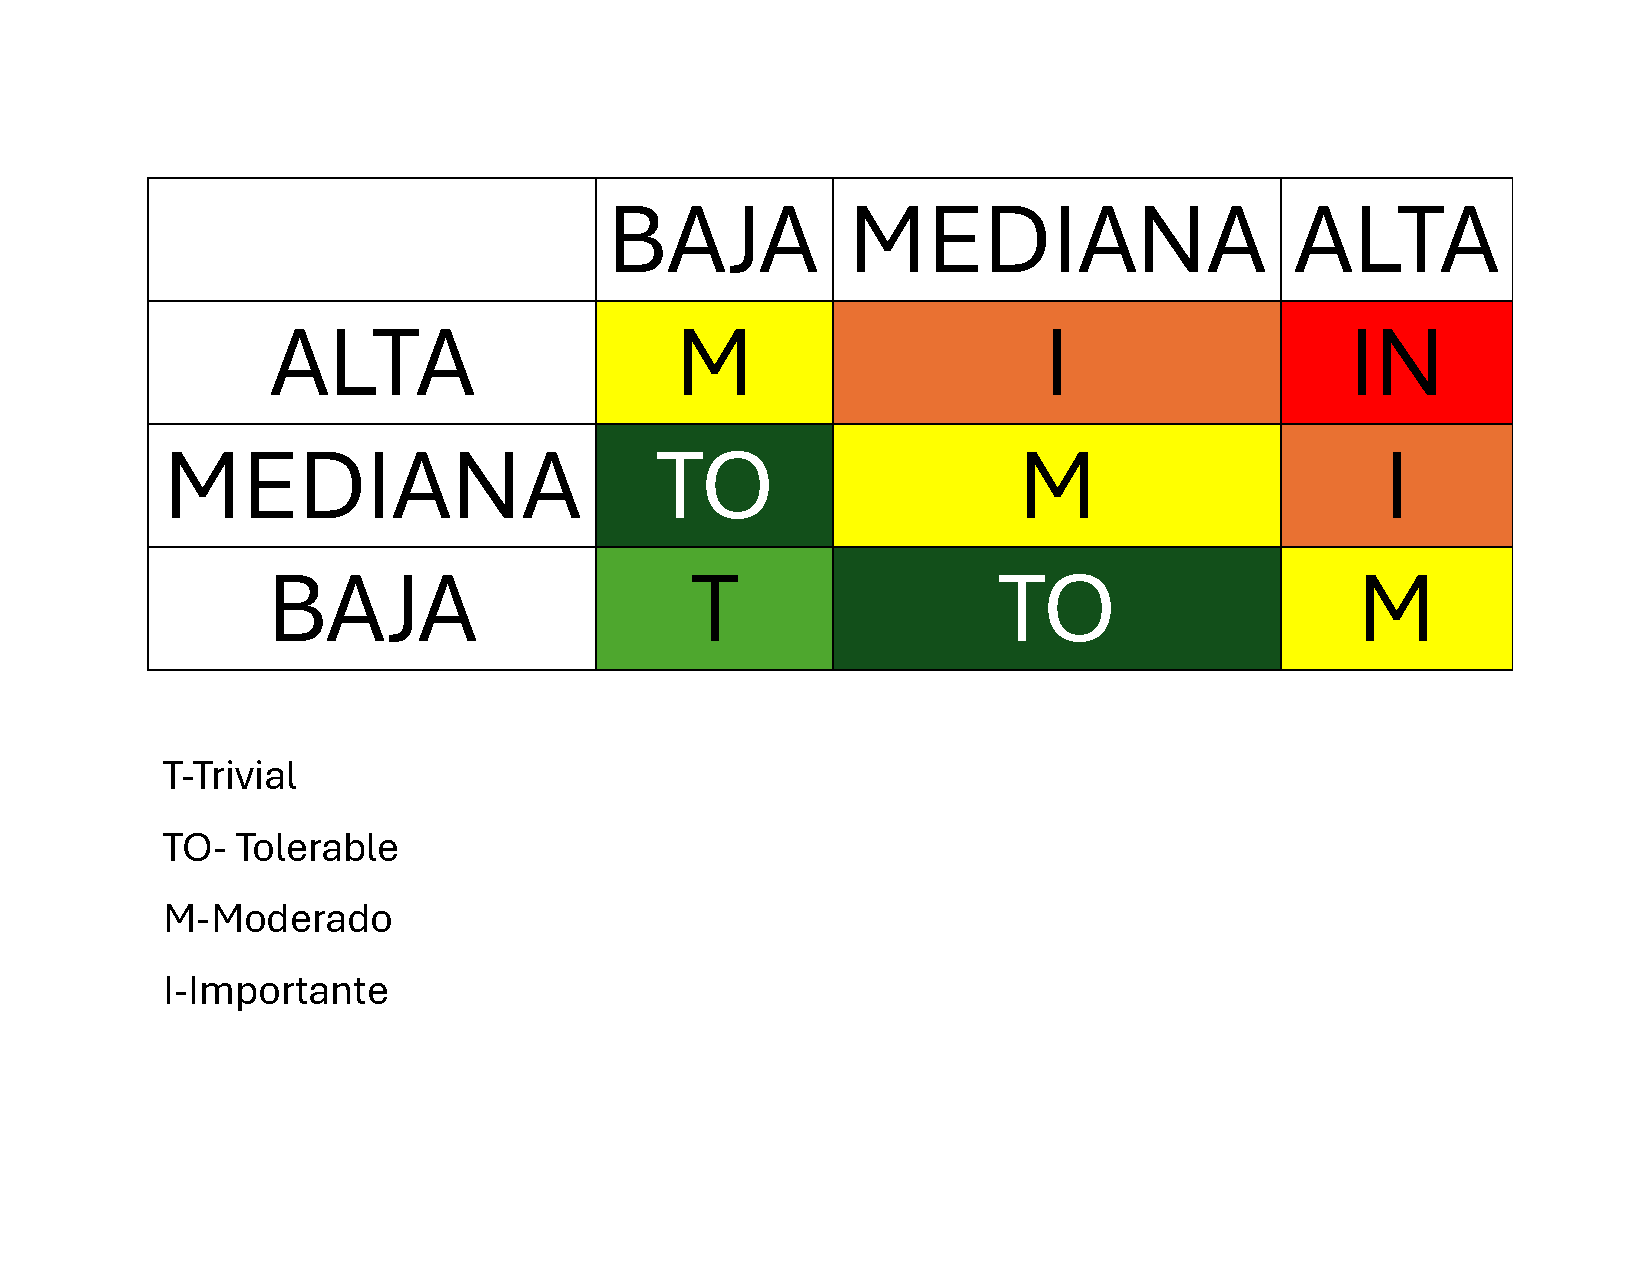
\includegraphics[scale=0.3]{13/img/EvaluacionRiesgo.pdf}
        \caption{Tabla de riesgos}
        % \label{fig:Tabla de riesgos}
    \end{figure}
    % 
    % 
    \subsubsection{Riesgos internos}
    
    Definimos el riesgo operativo interno como la posibilidad de que la empresa sufra como resultado de fallos naturales en su propio funcionamiento.
    
    \begin{figure}[H]
        \centering
        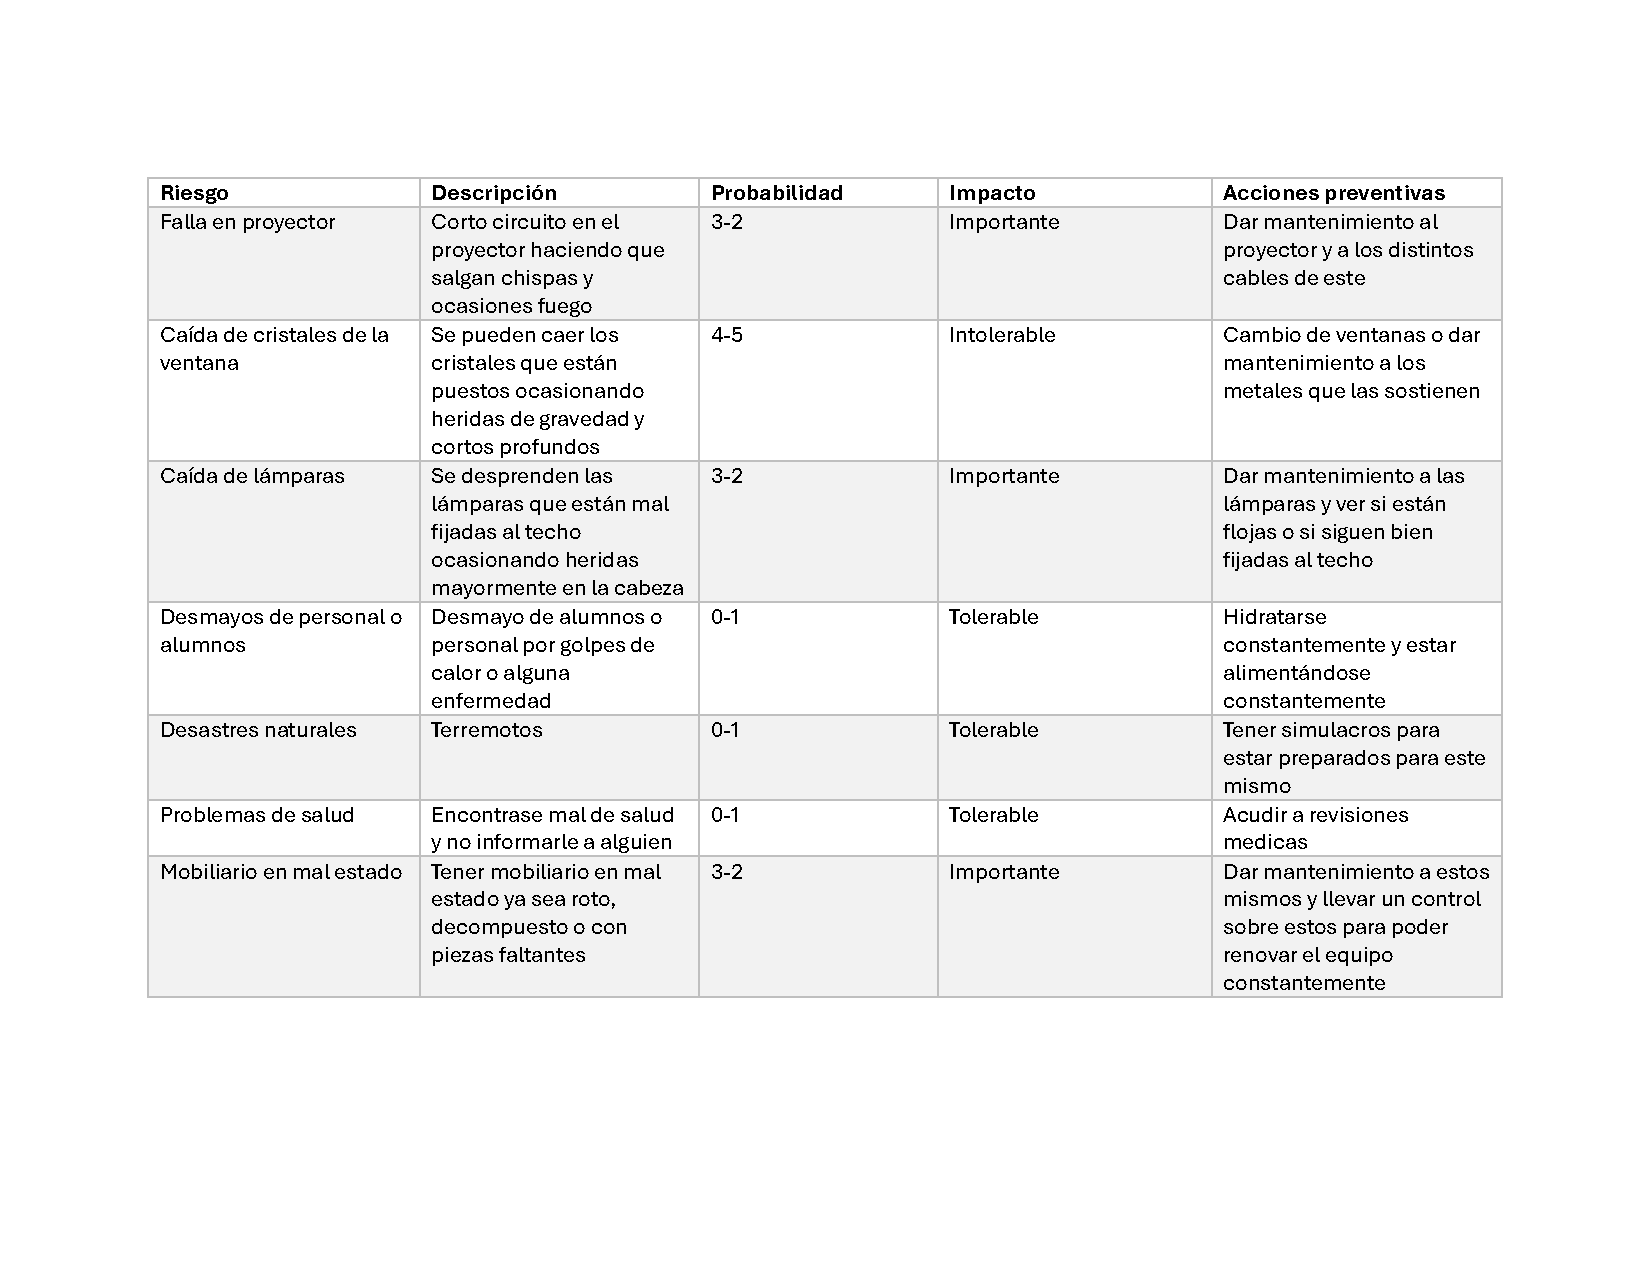
\includegraphics[scale=0.3]{13/img/riesgosInternos.pdf}
        \caption{Riesgos Internos}
        % \label{fig:Riesgos Internos}
    \end{figure}
    % 
    % 
    %\begin{table}[h]
        %\centering
       %% \caption{Riesgos con diferentes niveles y colores para distinguir la gravedad y acciones}
       % \begin{tabular}{c c c}
      %  \hline
       % \multicolumn{3}{c}{Riesgos}\\
      %  \hline
       %      Alto& 0.99 - 0.18 & Rojo  \\
      %  \hline
       %      Medio& 0.17 - 0.05 & Amarillo  \\
      %  \hline
       %      Bajo& 0.04 - 0.01 & Verde \\
      %  \hline     
      %  \end{tabular}
       % \label{tab:riego}
    %\end{table}
    % 
    % 
    % \begin{table}[h]
    %     \centering
    %     \caption{Descripción de los riesgos al realizar las actividades más comunes y de riesgo dentro de la empresa}
    %     \begin{tabular}{|c|c|c|c|p{7em}|c|}
    %          \hline
    %          Causa& Descripción del riesgo& Probabilidad& Impacto& Acciones Preventivas& Responsable \\
    %          \hline
    %          Gestión& Herida lacerada& 0.01 Bajo& Muy bajo& No utilizar navaja solo cúter&  \\
    %          \hline
    %          Gestión& Golpe con martillo& 0.01 Bajo& Muy bajo& Capacitación&  \\
    %          \hline
    %          Gestión& Levantar super sacos& 0.17 Medio& bajo& Utilizar faja y recibir ayuda&  \\
    %          \hline
    %          Gestión& Carga de camionetas& 0.01 Bajo& Muy bajo& Utilizar faja y guantes&  \\
    %          \hline
    %          Cliente& Descarga de camioneta& 0.17 medio& bajo& Utilizar faja y guantes&  \\
    %          \hline
    %          Gestión& Corto circuito& 0.17 medio& bajo& Revisar las conexiones de la fuente de energía cada mes&  \\
    %          \hline
    %          Cliente& Fumador& 0.01 Bajo& Muy bajo& Señalamientos y llamada de atención&  \\
    %          \hline
    %     \end{tabular}
    %     \label{tab:Riesgos}
    % \end{table}
    % 
    % 
    %\begin{figure}[H]
       % \centering
       % \includegraphics[trim = {20mm 130mm 20mm 46mm},clip,scale=0.45]{6/Img/riesgos0.pdf}
      %  \caption{Descripción de los riesgos al realizar las actividades más comunes y de riesgo dentro de la empresa}
        % \label{fig:my_label}
    %\end{figure}
    % 
    % 
    \subsubsection{Riesgos externos}
    \begin{figure}[H]
        \centering
        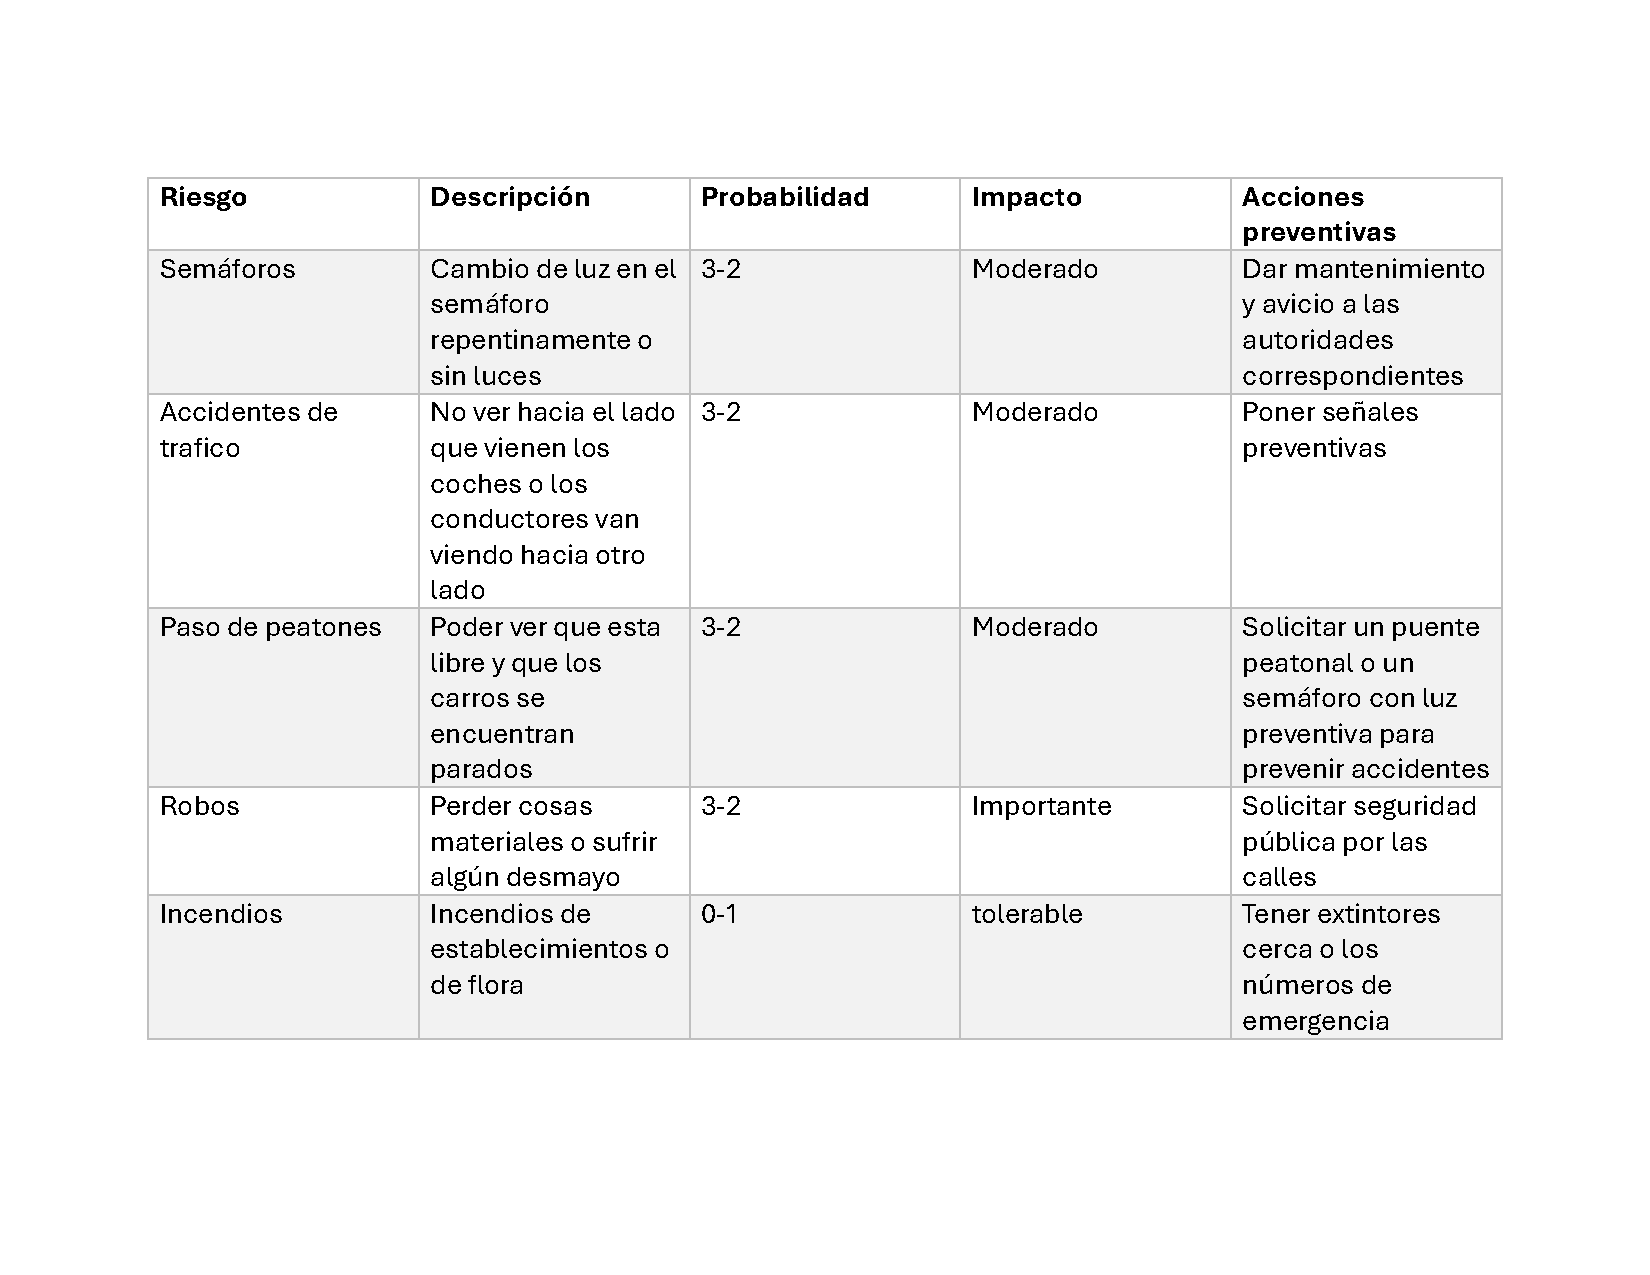
\includegraphics[scale=0.3]{13/img/riesgoExternos.pdf}
        \caption{Riesgos Externos}
        % \label{fig:Riesgos Externos}
    \end{figure}
    % \begin{table}[H]
    %     \centering
    %     \caption{Descripción de los riesgos externos}
    %     \begin{tabular}{|c|c|c|p{10em}|}
    %          \hline
    %          Descripción del riesgo& Probabilidad& Impacto& Acciones preventivas\\
    %          \hline
    %          Desmayo del cliente& 0.01 bajo& Muy bajo& Colocar al cliente en una posición apropiada para la llegada de los paramedicos\\
    %          \hline
    %          Incendio de algún vecino& 0.01 bajo& Alto& Mantener los detectores de humo en lugares estratégicos y con pilas\\
    %          \hline
    %          Incendio de camioneta& 0.17 moderado& Alto& Mantener en mantenimiento los sensores de temperatura y con un extintor \\
    %          \hline
    %          Incendio por pirotecnia& 0.17& Alto& Vigilar en los días festivos y mojar el material\\
    %          \hline
    %          Choque en la avenida& 0.17& Medio& Delimitar y poner conos de señalamiento\\
    %          \hline
    %     \end{tabular}
    %     \label{tab:RiesgosExternos}
    % \end{table}
    % 
    % 
    %\begin{figure}[H]
       % \centering
        %\includegraphics[trim = {20mm 136mm 20mm 43mm},clip,scale=0.5]{6/Img/riesgoExt.pdf}
       % \caption{Descripción de los riesgos externos}
       % \label{fig:riesgoExt}
    %\end{figure}
    % 
    % 
    \subsubsection{Programa de actividades de prevención y auxilio}
    
    Es fundamental contar con un programa de apoyo en cualquier organización para garantizar la protección y el bienestar de las personas, así como la continuidad de las operaciones en caso de emergencias o desastres.Por lo tanto, estas son las acciones de prevención que se toman antes de que ocurra un incidente.
    
    % 
    % 
    \subsubsection{Plan de acción}
    
    El plan de acción del ITQ es un conjunto estratégico de instrucciones para abordar problemas y gestionar riesgos internos y externos. La identificación y prevención de riesgos se incluyen en este plan mediante la anticipación y mitigación de amenazas potenciales. Además, establece procedimientos y responsabilidades claros para responder a incidentes. Además, incluye la gestión de recursos, que implica identificar los recursos necesarios y establecer plazos para la ejecución de las medidas establecidas. Además, se implementan planes de seguimiento y evaluación continua del plan para garantizar la preparación y la seguridad de la comunidad universitaria. En resumen, el plan de acción proporciona instrucciones claras y detalladas para administrar riesgos y responder a emergencias en el ITQ. 
    \begin{figure}[H]
        \centering
        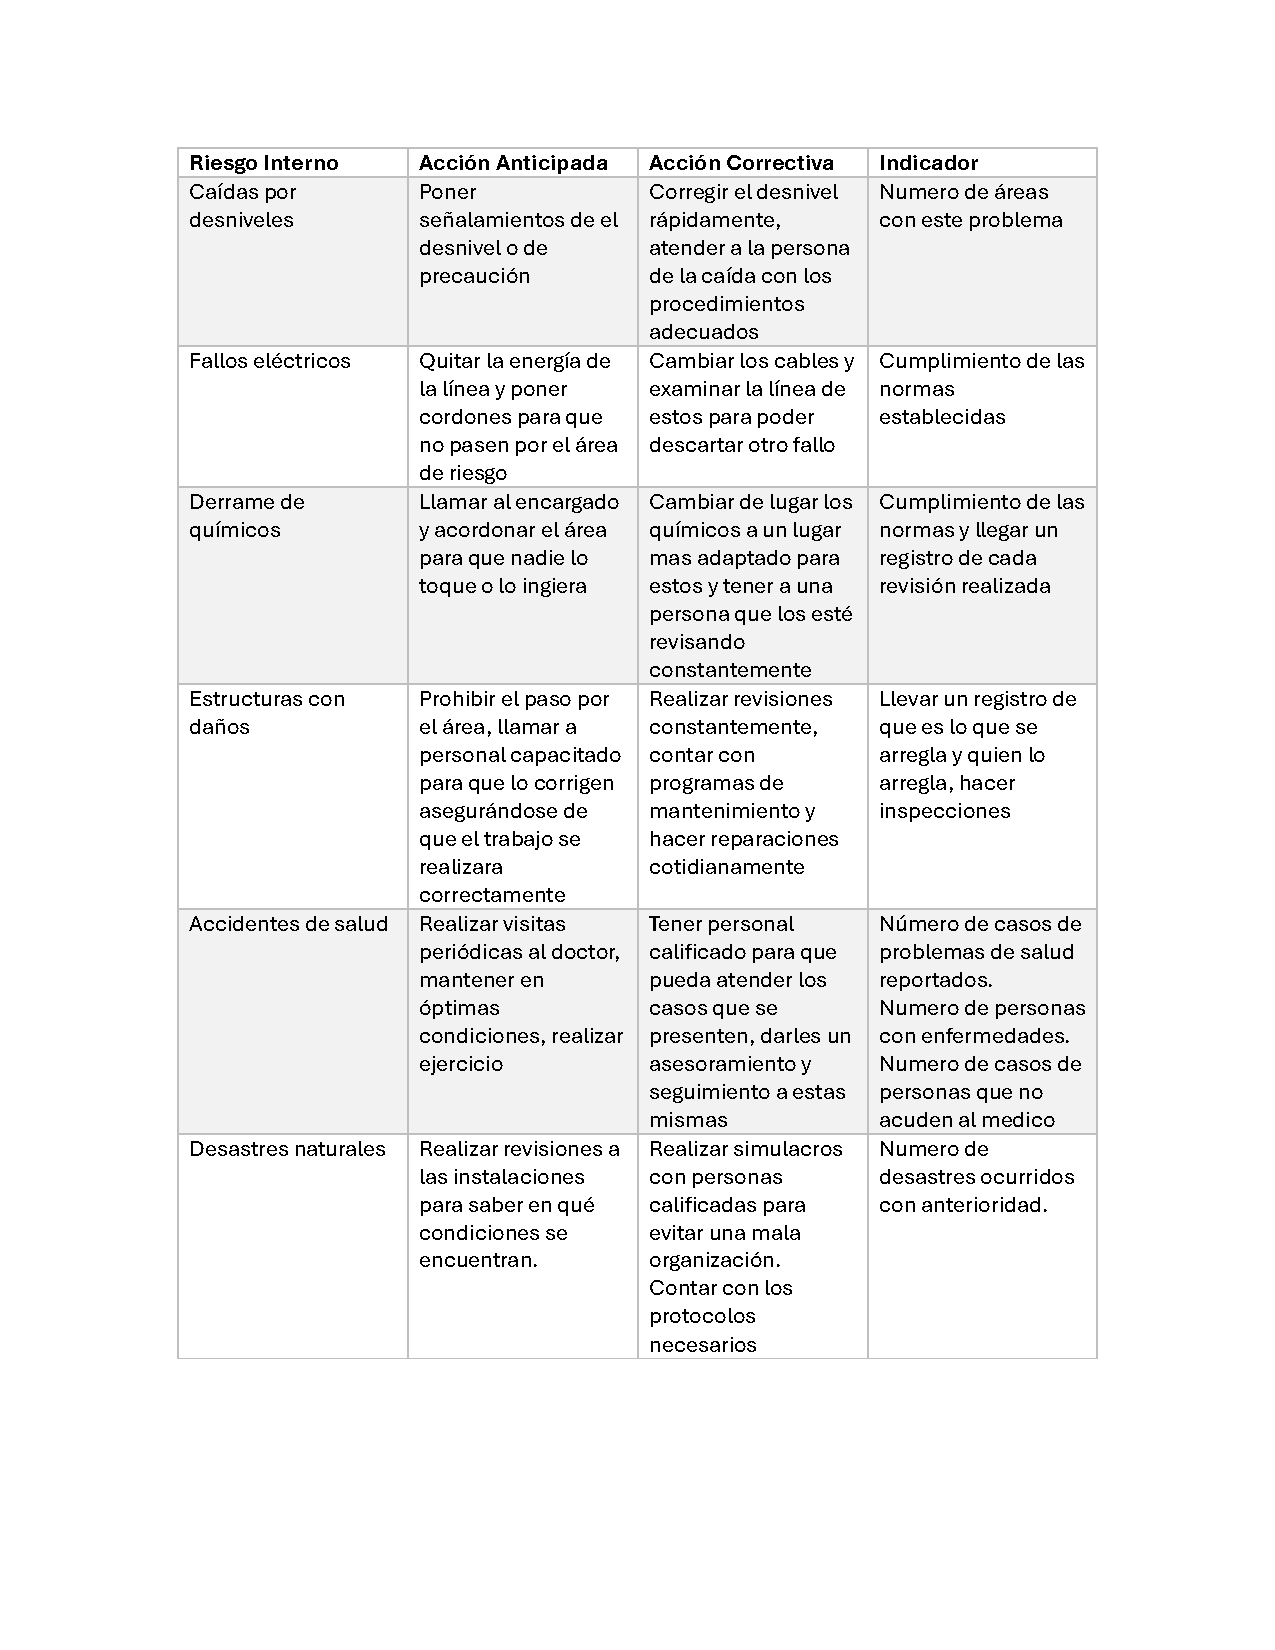
\includegraphics[scale=0.3]{13/img/planDeAccion.pdf}
        \caption{Plan de accion }
        % \label{fig:Plan de accion interno}
    \end{figure}
    \begin{figure}[H]
        \centering
        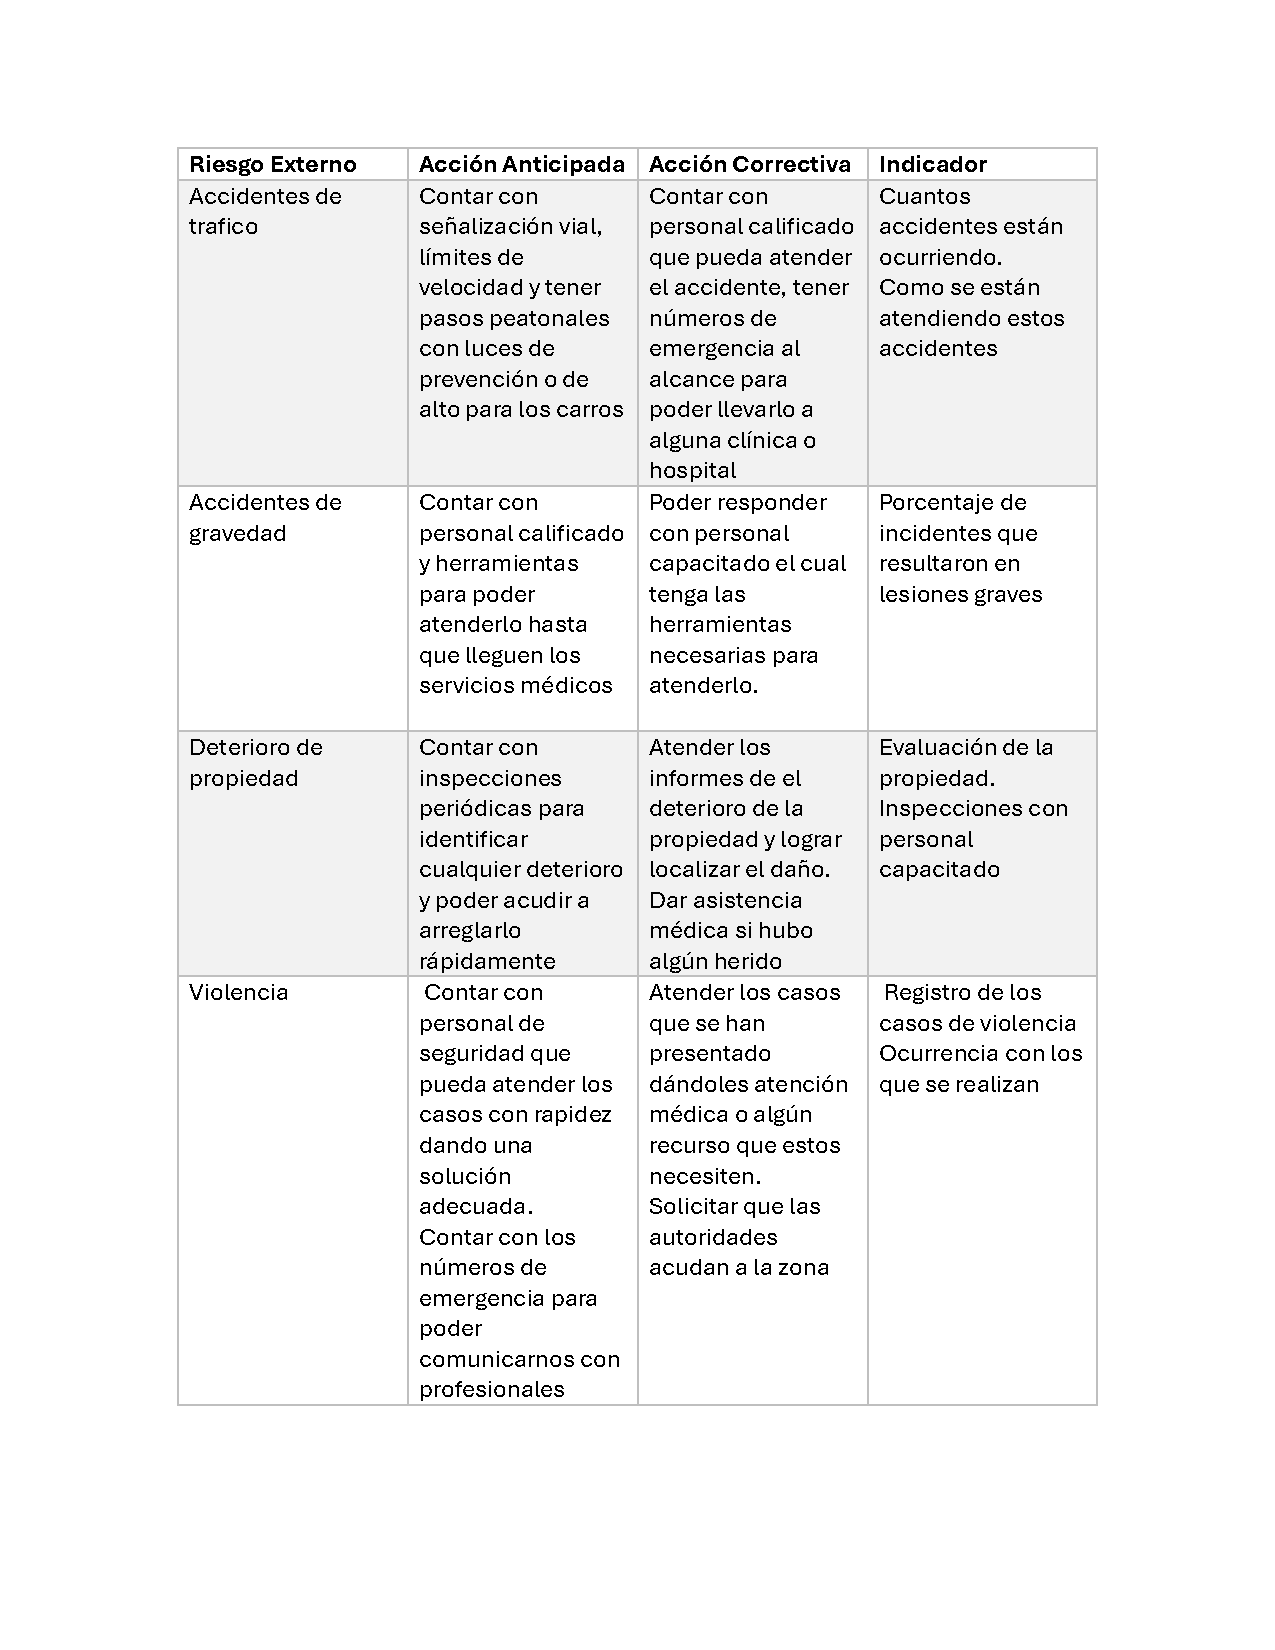
\includegraphics[scale=0.3]{13/img/planDeAccionDos.pdf}
        \caption{Plan de accion}
        % \label{fig:Plan de accion externo}
    \end{figure}
    % 
    % 
    % \begin{table}[H]
    %     \centering
    %     \caption{Descripción de las acciones anticipadas y correctivas ante un riesgo interno}
    %     \begin{tabular}{|p{5em}|p{10em}|p{11em}|p{10em}|}
    %         \hline
    %          RIESGO INTERNO& Acción Anticipada& Acción Correctiva& Indicador\\
    %          \hline
    %          Herida lacerada& Reemplazar las navajas y cuchillos por cutter con resorte. Utilizar en lo menos posible objetos punzo cortantes& Utilizar el material de los primeros auxilios y lavar la herida con agua oxigenada y vendar& Constancias de capacitación así como el registro de la disminución en el uso de curitas\\
    %          \hline
    %          Golpeo con martillo& Capacitación y descansos de 5 minutos cuando se este trabajando constantemente con el martillo& Aplicar pomada para golpes del botiquín de primeros auxilios& Menos reportes de golpes\\
    %          \hline
    %          Levantar super sacos& Capacitar con el uso adecuado de la faja y solicitar ayuda al momento de levantar materiales mayores a 30 kg& Tomar un descanso y tomar agua &Disminución del cansancio al final del día\\
    %          \hline
    %          Carga y descarga de camionetas& Capacitar con el uso adecuado de la faja y solicitar ayuda al momento de levantar materiales mayores a 30 kg& Utilizar más personal para evitar riesgos & Menor tiempo de carga y descarga en la camioneta\\
    %          \hline
    %          Chispa por cigarro& Señalamientos de no fumar a la entrada& Pedir de manera amable que apaguen el cigarro& Observar en el área de trabajo decremento de las colillas de cigarro\\
    %          \hline
    %          Corto circuito& Mantenimiento preventivo en los fusibles en el centro de carga& Bajar los interruptores del centro de carga& Obtención de un reporte técnico por lo menos una vez al año\\
    %          \hline
    %     \end{tabular}
    %     \label{tab:my_label}
    % \end{table}
    % 
    % 
    %\begin{figure}[H]
       % \centering
        %\includegraphics[trim = {20mm 82mm 20mm 25mm},clip,scale=0.45]{6/Img/accionAntInterno.pdf}
        %\caption{Descripción de las acciones anticipadas y correctivas ante un riesgo interno }
        %\label{fig:accionAntInterno}
    %\end{figure}
    % 
    % 
    % \begin{table}[H]
    %     \centering
    %     \caption{Descripción de las acciones anticipadas y correctivas ante un riesgo externo e interno}
    %     \begin{tabular}{|p{5em}|p{10em}|p{11em}|p{10em}|}
    %          \hline
    %          RIESGO EXTERNO& Acción Anticipada& Acción Correctiva& Indicador\\
    %          \hline
    %          Desmayo del cliente& Tomar cursos de primeros auxilios por lo menos una vez al año a todo el personal& Contar con los conocimientos básicos de primeros auxilios& Realizar un simulacro que nos permita evaluar las acciones en el manejo del riesgo por desmayo\\
    %          \hline
    %          Incendio de algún vecino& Mantener los detectores de humo en lugares estratégicos y cambiar las pilas cada 2 meses& Llamar al 911 para informar del incendio y del posible riesgo en el negocio&  Llevar un registro de los cambios de las pilas en los detectores de humo\\
    %          \hline
    %          Incendio de camioneta& Mantener en mantenimiento los sensores de temperatura y con un extintor& Accionar el extintor conforme a lo establecido por el departamento de bomberos y llamar al 911& Revisar el tablero de la camioneta que no indique falta de agua o alta temperatura \\
    %          \hline
    %          Incendio por pirotecnia& Vigilar en los días festivos y mojar el material& Llamar a emergencias y tratar de sofocar el fuego& Hacer un llamado a los vecinos a ser cuidadosos\\
    %          \hline
    %          Choque en la avenida& Delimitar y poner conos de señalamiento& Llamar a emergencias y si es que hay daños a personas, aplicar primeros auxilios en caso de ser necesario& Llevar un registro de las horas pico para evitar hacer maniobras\\
    %          \hline
    %     \end{tabular}
    %     \label{tab:Acciones}
    % \end{table}
    % 
    % 
    %\begin{figure}[H]
      %  \centering
       % 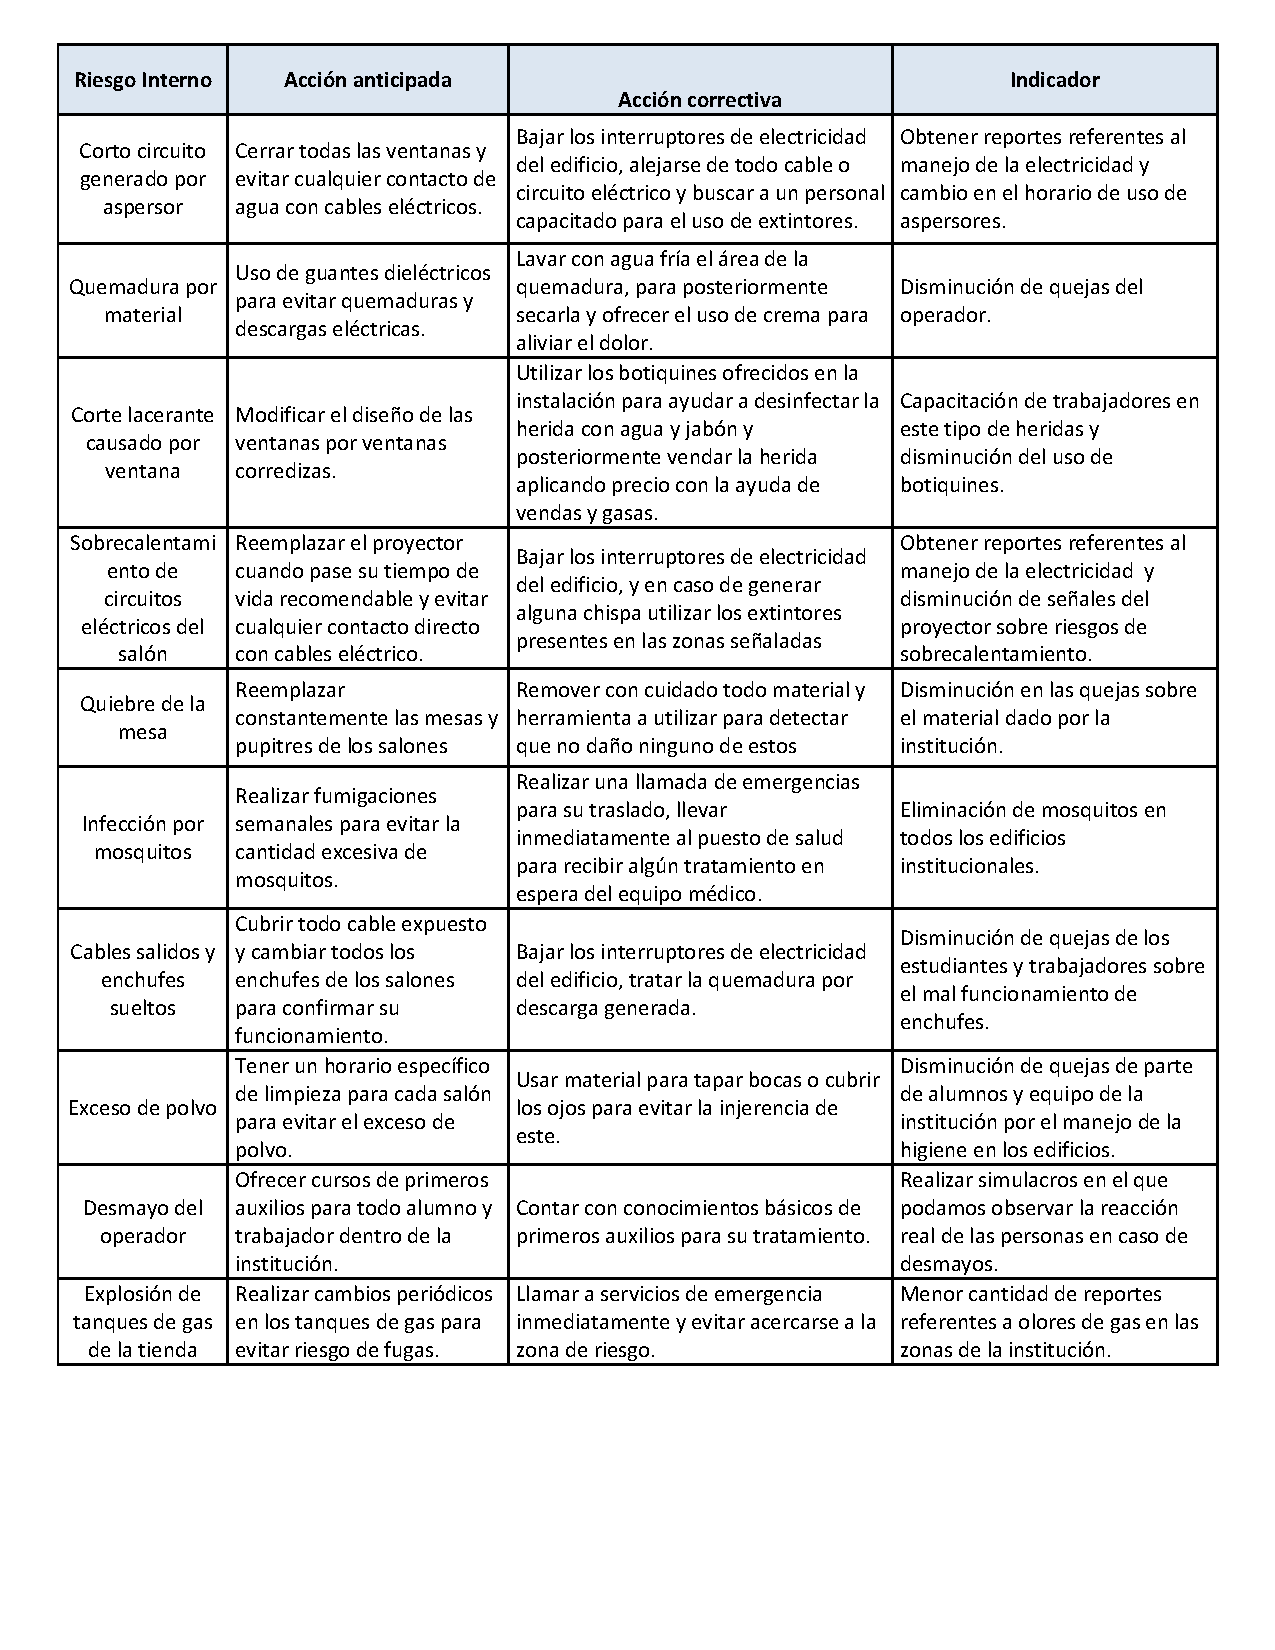
\includegraphics[trim = {20mm 125mm 20mm 25mm},clip,scale=0.45]{6/Img/accionAnti.pdf}
       % \caption{Descripción de las acciones anticipadas y correctivas ante un riesgo externo}
       % \label{fig:accionAnti}
    %\end{figure}
    % 
    % 
    % Cada estrategia metodológica se establece acorde a cada objetivo, y por tanto deberá ser desglosada precisada y ordenada claramente. En consecuencia cada objetivo que se presentó en forma de verbo en infinitivo deberá determinar una estrategia en forma de adverbio. Ej. Desarrollar…Desarrollo. Son las actividades ordenadas que tienen como finalidad la prueba de la hipótesis. 
    
    % \begin{itemize}
    %     \item Se debe establecer que se habrá de hacer, como, conque, y donde para obtener la información que permita probar la hipótesis.  
    %     \item Se debe desglosar de acuerdo a los objetivos específicos. 
    %     \item Se debe establecer una estrategia metodológica por cada objetivo específico. De manera simplista se podría decir que se cambia el verbo en infinitivo por su respectivo adverbio.
    %     \item En cada objetivo se debe describir que método, que materiales y que equipo se usará para conseguirlo.
    %     \item Se deben tener referencias Figura \ref{fig:lcd-16x2}.
    % \end{itemize}
    % 
    % 
    % \begin{figure}[H]
    %     \centering
    %     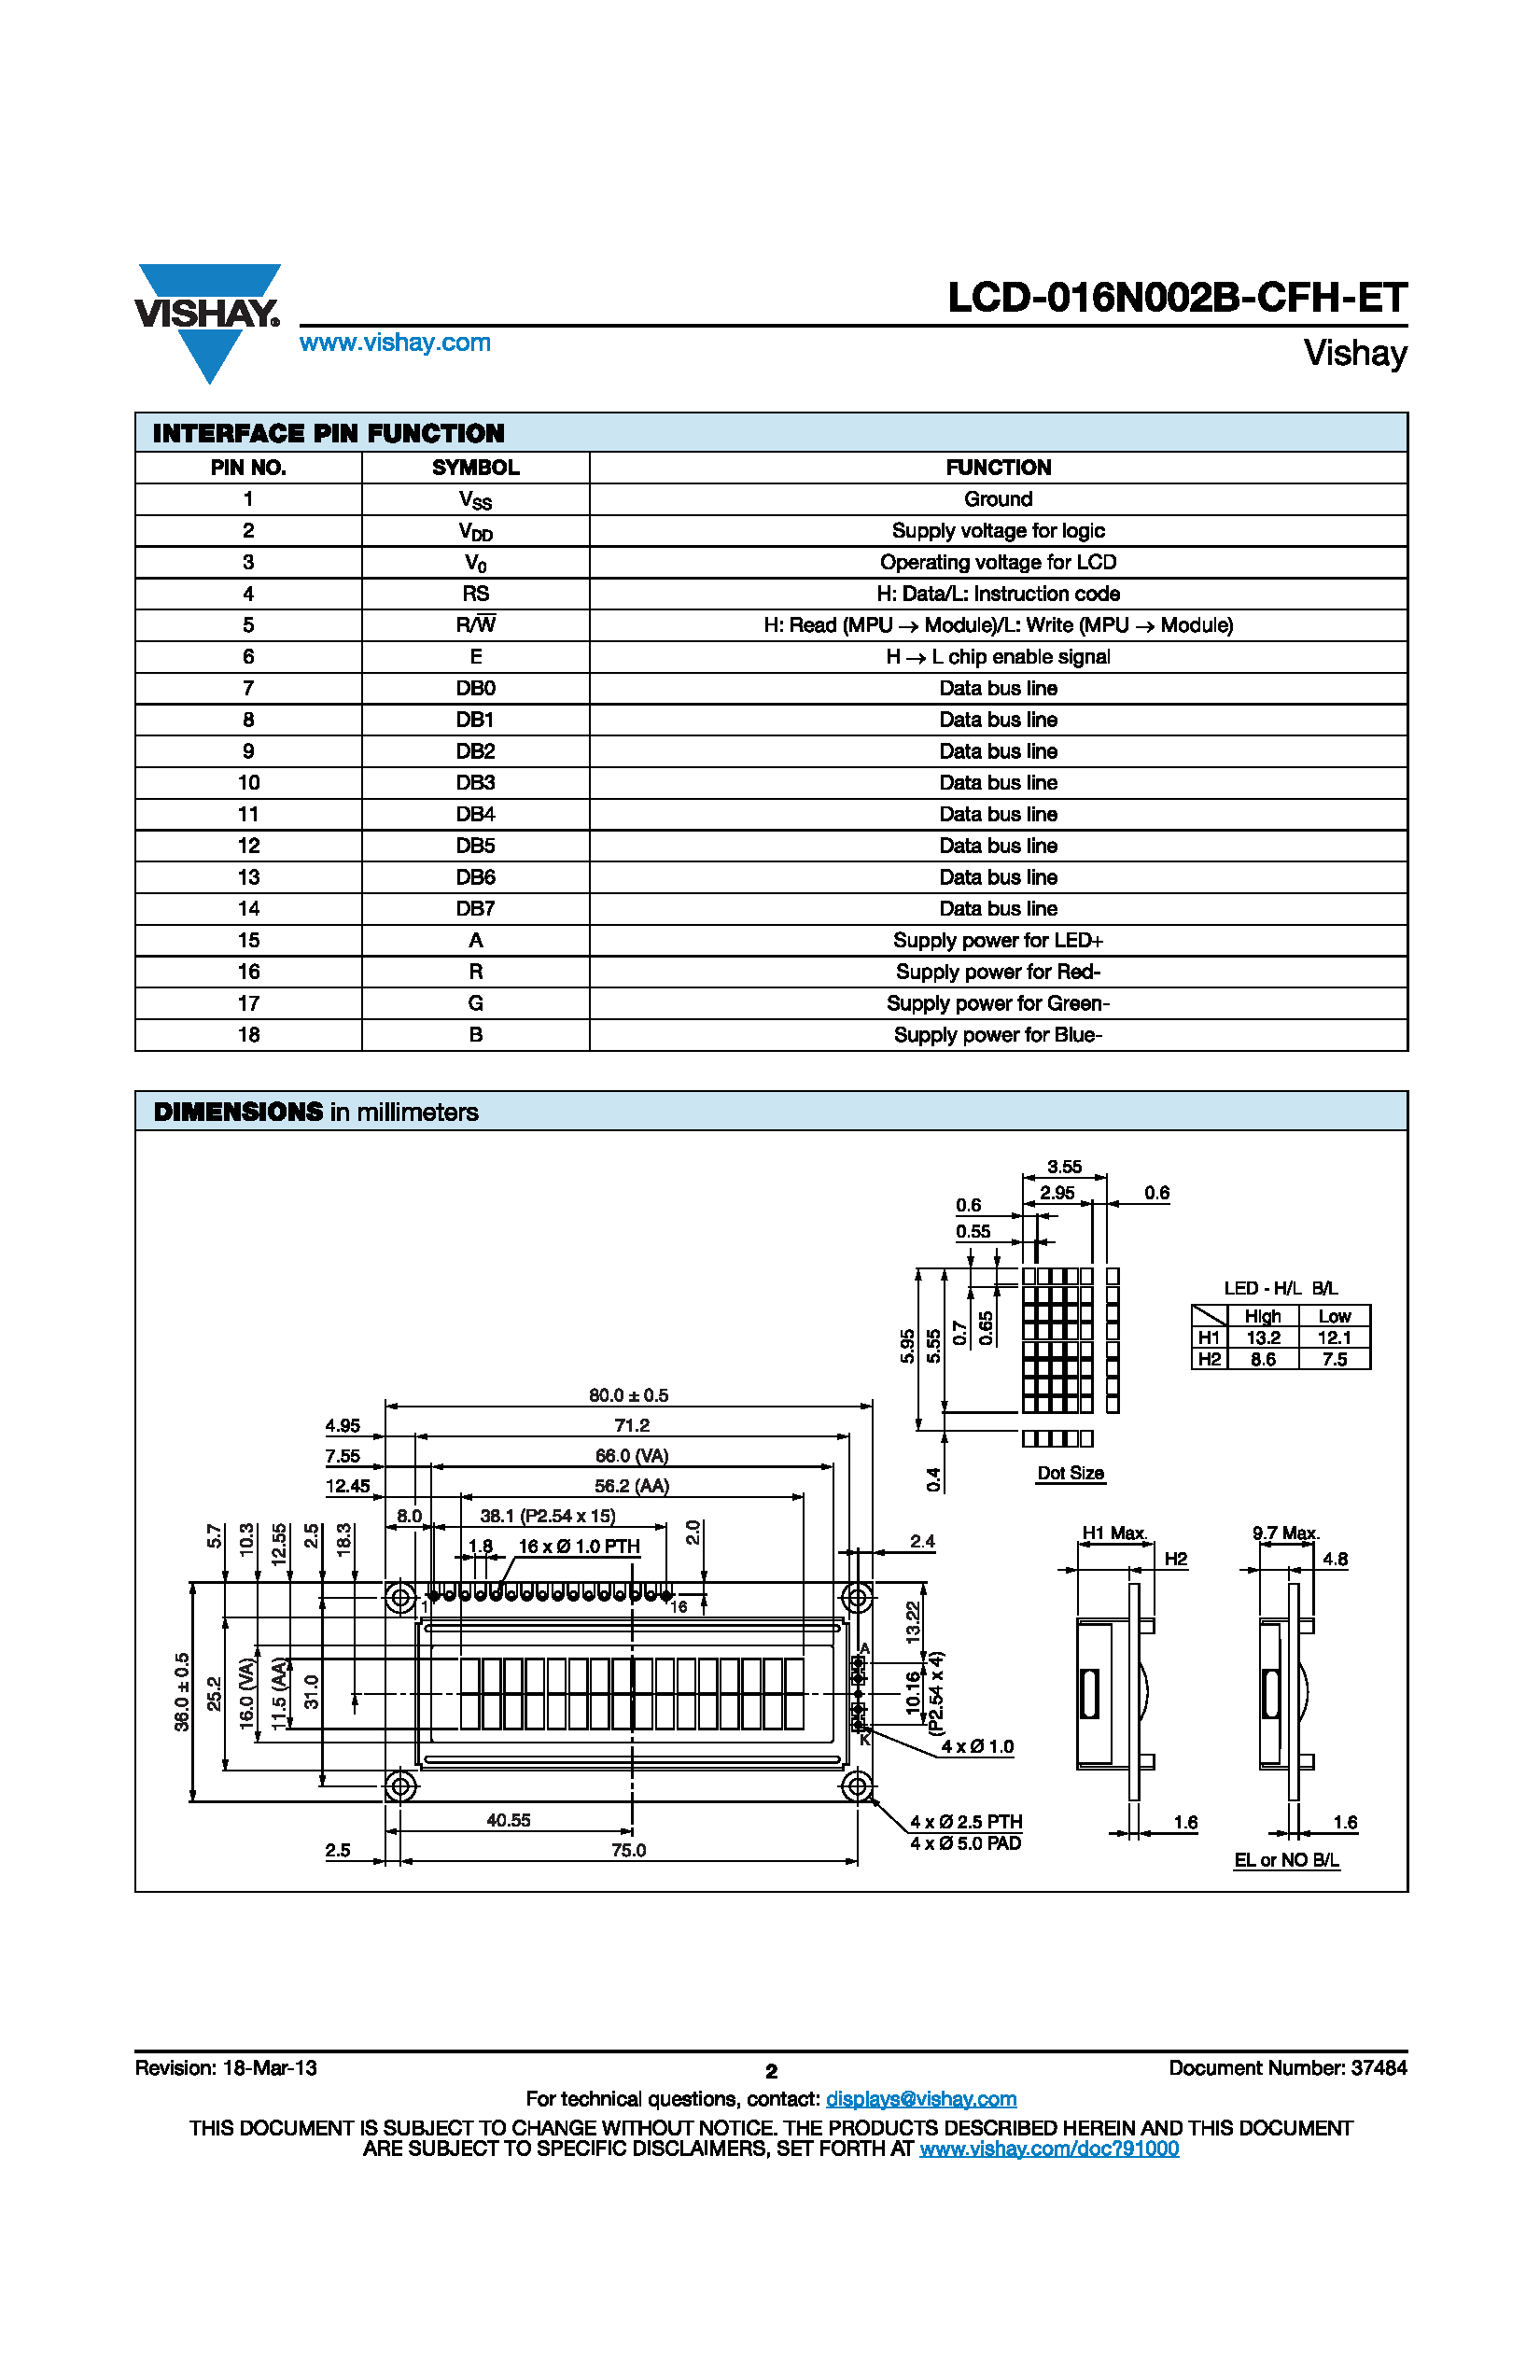
\includegraphics[trim = {30mm 65mm 90mm 250mm},clip,scale=0.5]{6/Img/lcd-16x2.pdf}
    %     \caption{Esquema LCD de 16x2}
    %     \label{fig:lcd-16x2}
    % \end{figure}
    % 
    % 
    % \begin{figure}[H]
    %     \centering
    %     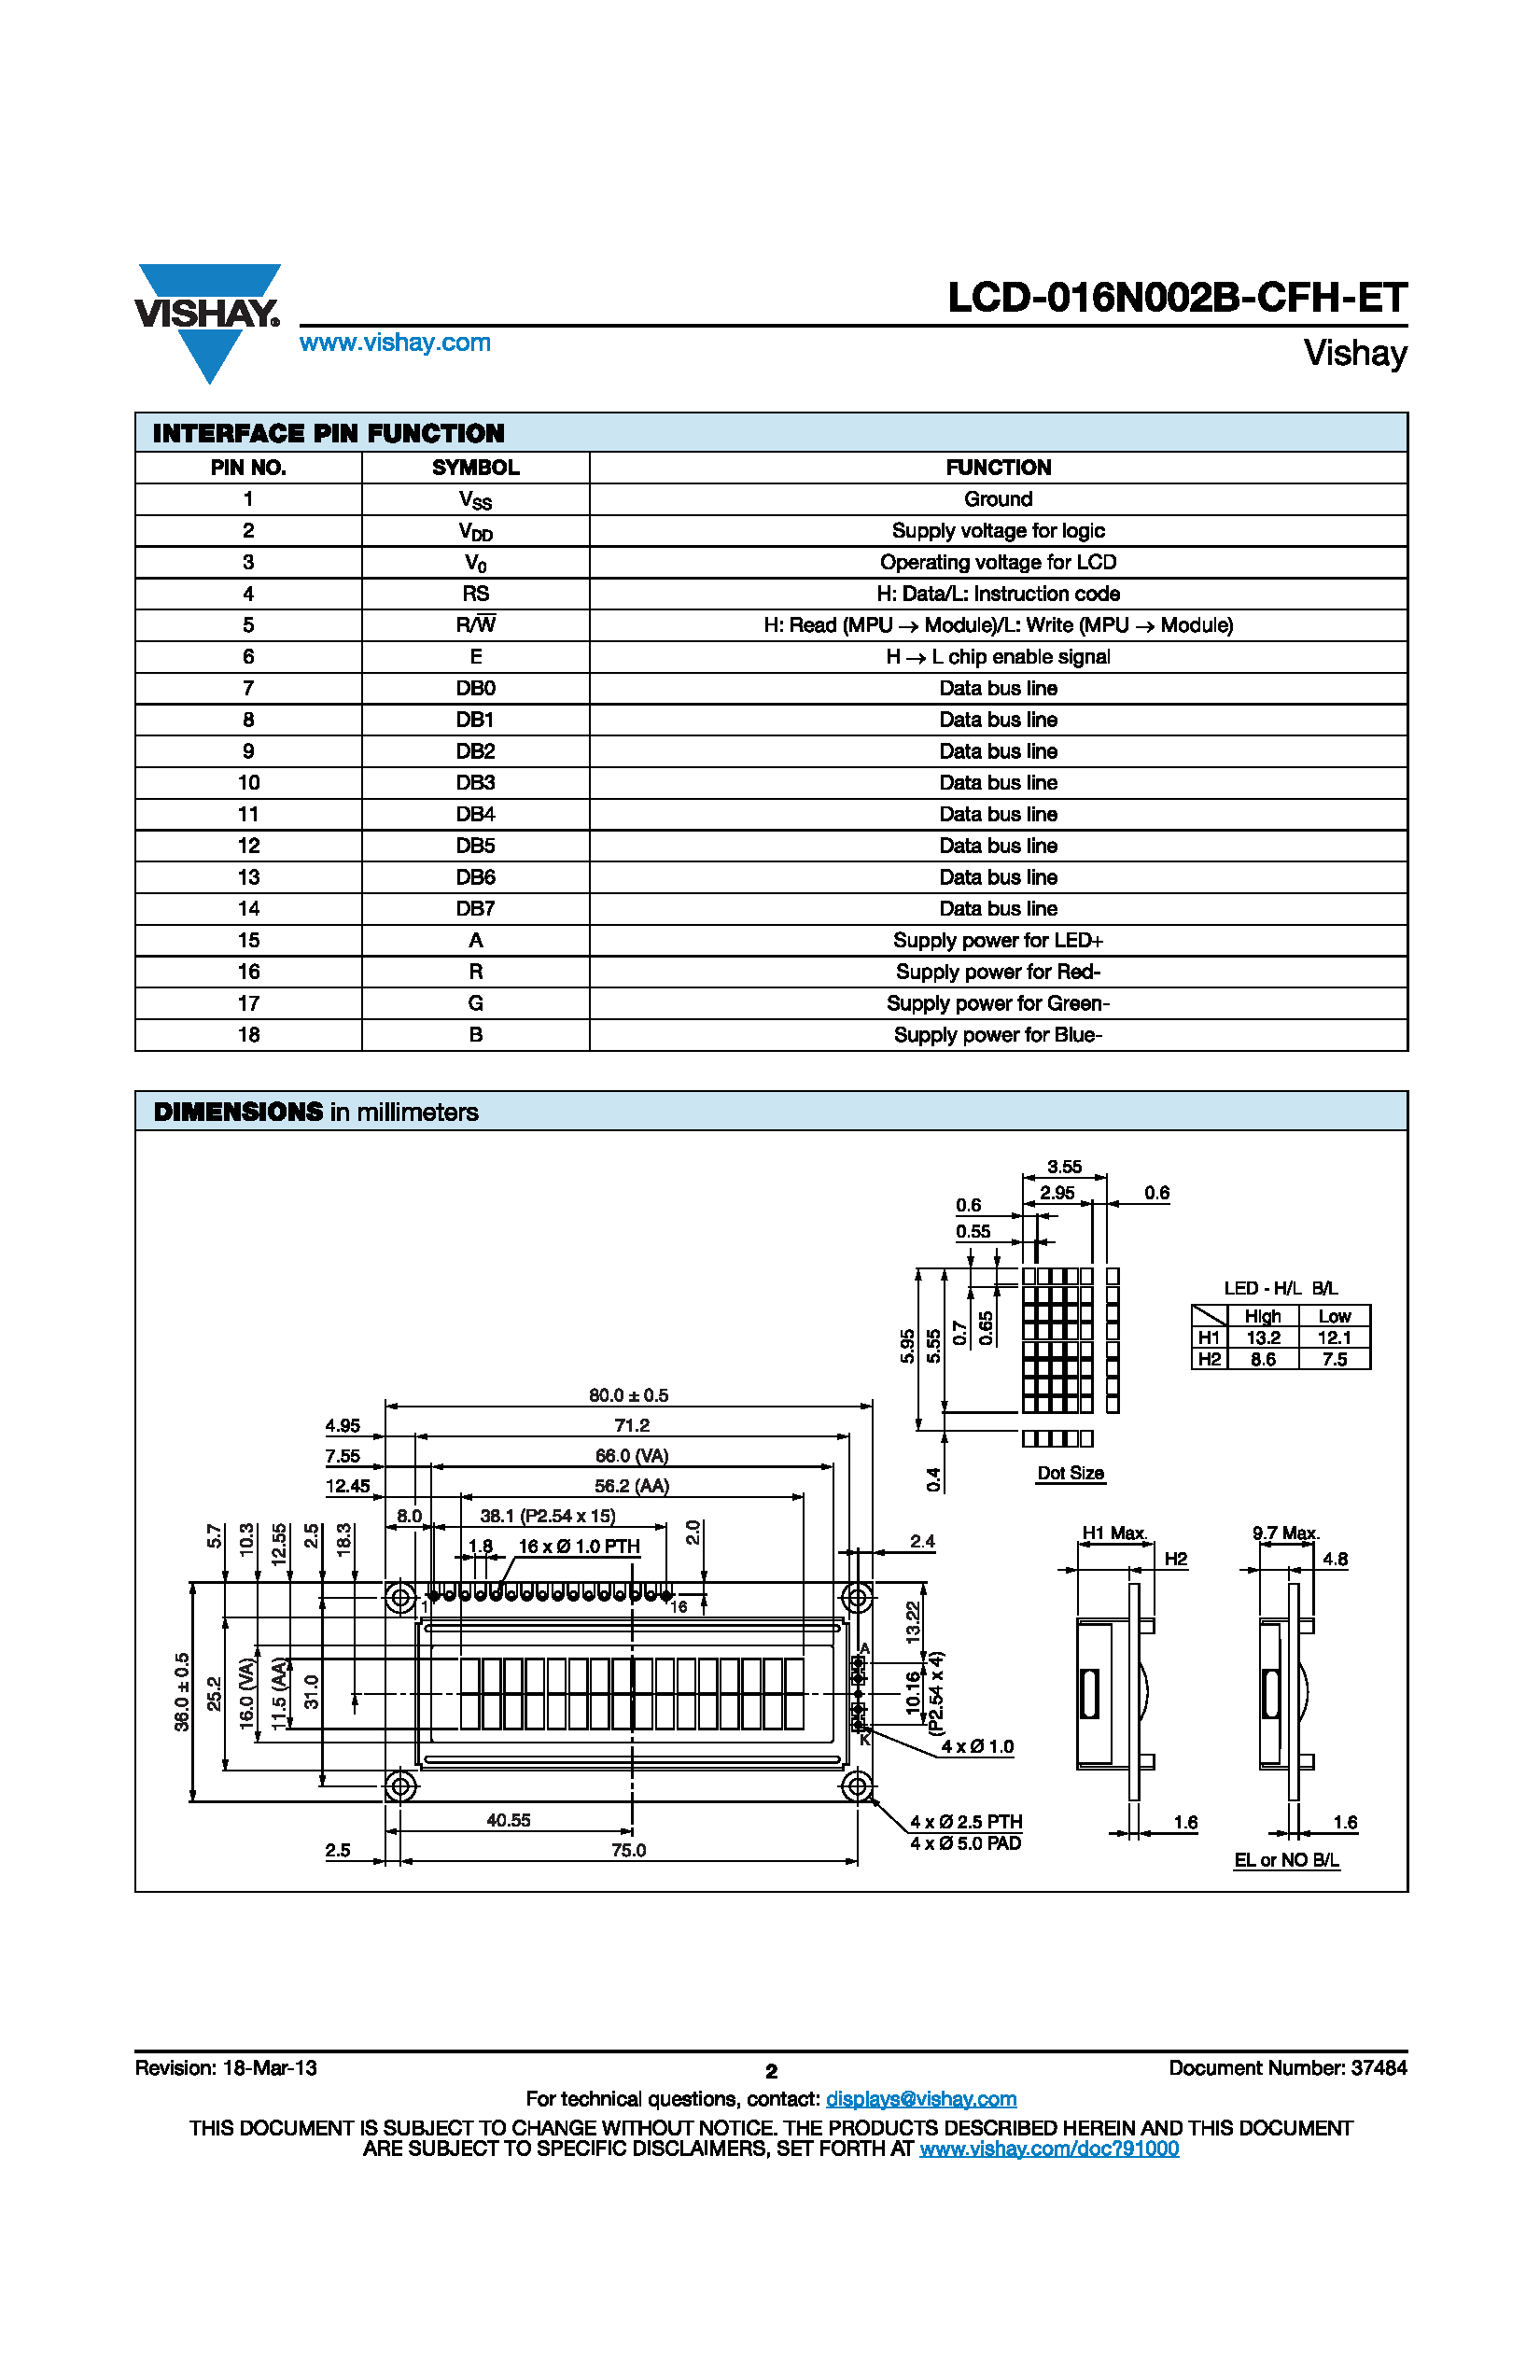
\includegraphics[trim = {30mm 250mm 90mm 20mm},clip,scale=0.5]{6/Img/lcd-16x2.pdf}
    %     \caption{Esquema LCD de 16x2}
    %     \label{fig:lcd}
    % \end{figure}
    % 
    % 
    % \subsection{Prepara tu documento}
    
    % Antes de que comiences a utilizar esta plantilla, es recomendable que prepare la información que contendrá en un archivo aparte. 
    % Ten preparadas tus gráficas, así como también las tablas aparte, para que sea más fácil integrarlo. 
    % Se recomienda fuertemente el uso de \textbf{formato Enhanced Metafile (.emf) para imágenes y gráficas} de resolución óptima. 
    % Finalmente, completa y organiza el contenido antes de darle el formato de esta plantilla. 
    % 
    % 
    \subsubsection{Identificación de capacidades}
    
    \begin{table}[H]
        \centering
        \caption{Recursos en materia de seguridad}
        \begin{tabular}{c c c}
        \hline
        \multicolumn{3}{c}{Inventario de recursos en materia de seguridad}\\
        \hline
             No.& Recurso & Cantidad  \\
        \hline
             1& Extintor & 6  \\
        \hline
             2& Botiquín & 3  \\
        \hline
             4& Áreas seguras & 3 \\
        \hline     
        \end{tabular}
        \label{tab:inventario}
    \end{table}
    % 
    % 
    \subsubsection{Plano de localización de recursos}
    
    % 
    \begin{figure}[H]
        \centering
        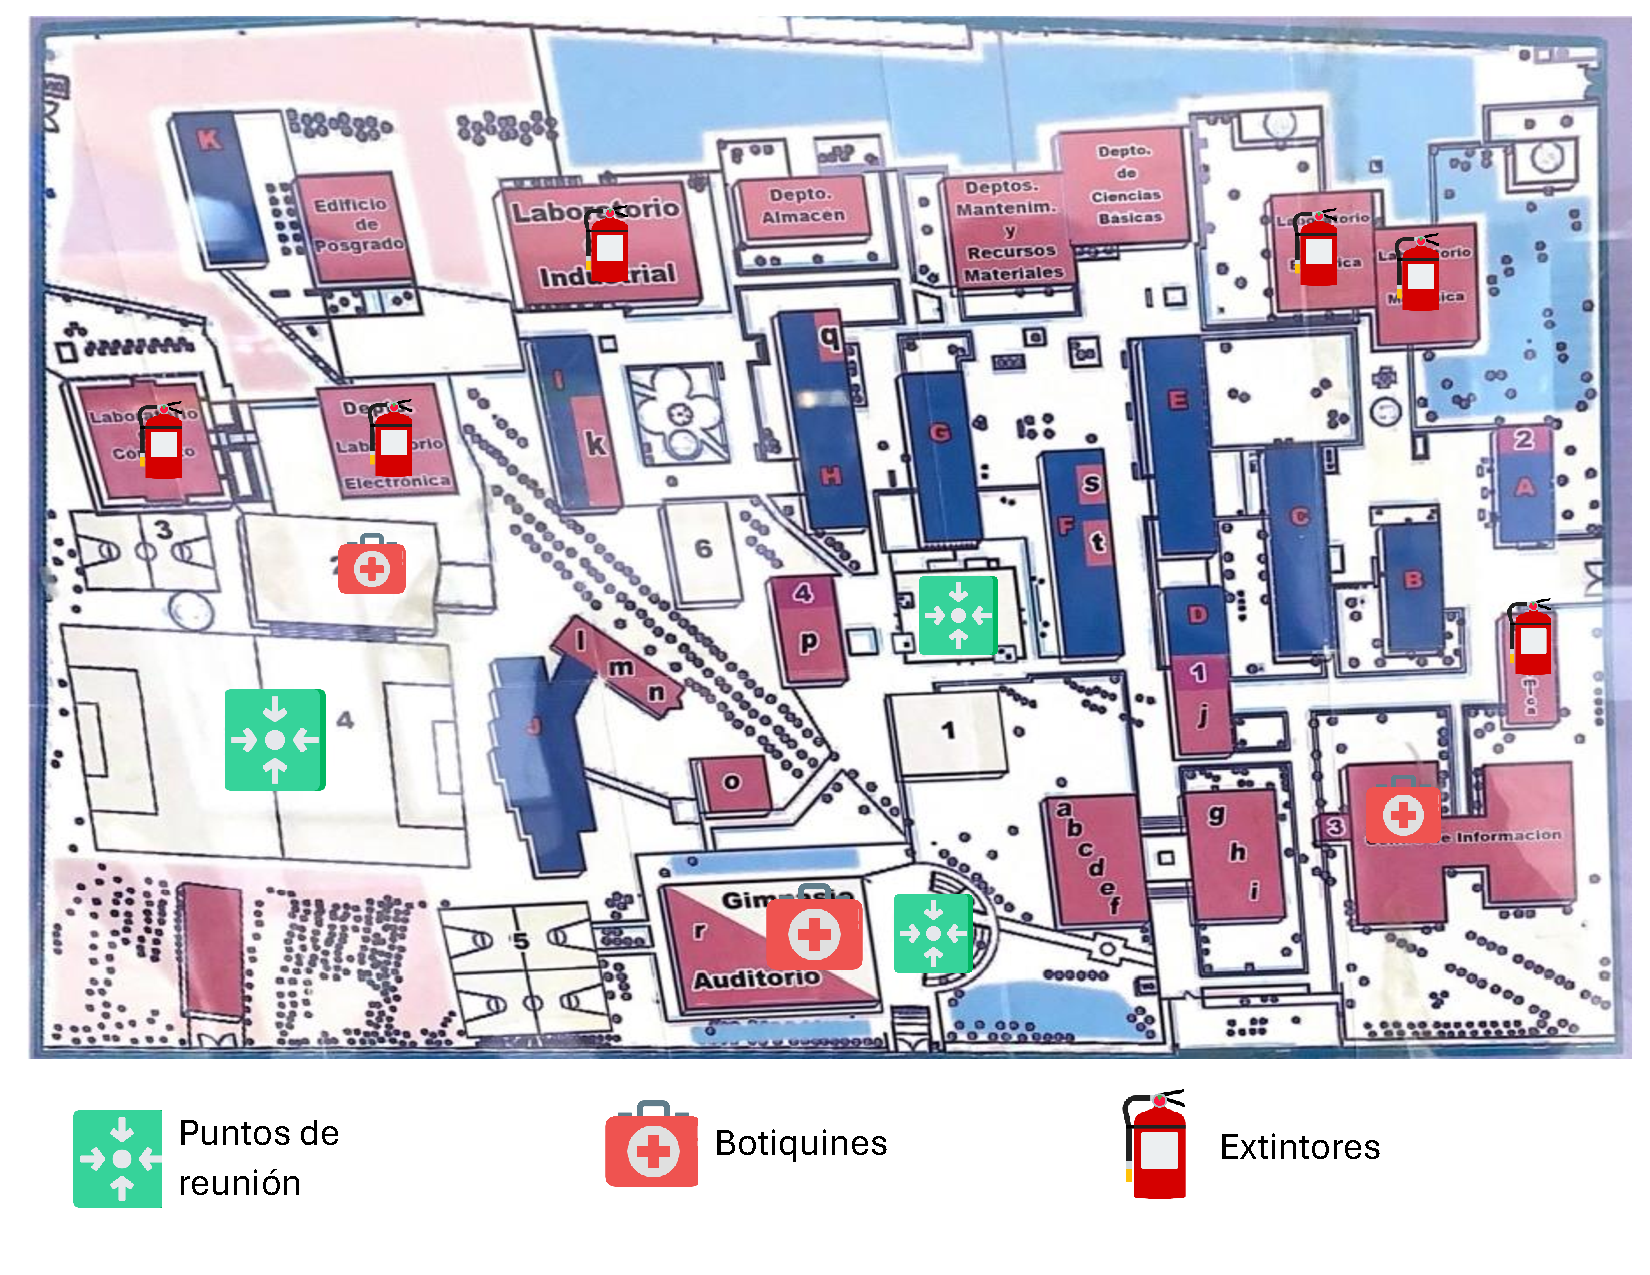
\includegraphics[scale=0.25]{13/img/localizacionDeRecursos.pdf}
        \caption{Plano de localización de recursos}
        % \label{fig:Plano de localizacion de recursos}
    \end{figure}
    % 
    %\begin{figure}[H]
       % \centering
       % \includegraphics[trim = {20mm 25mm 20mm 12mm},clip,scale=0.3]{6/Img/PlanoLocalizaciónRecursos.pdf}
       % \caption{Plano del establecimiento de los recursos en materia de seguridad.}
       % \label{fig:PlanoLocalizaciónRecursos}
    %\end{figure}
    % 
    % 
    \subsubsection{ Identificación de apoyos externos}
    
    \begin{figure}[H]
        \centering
        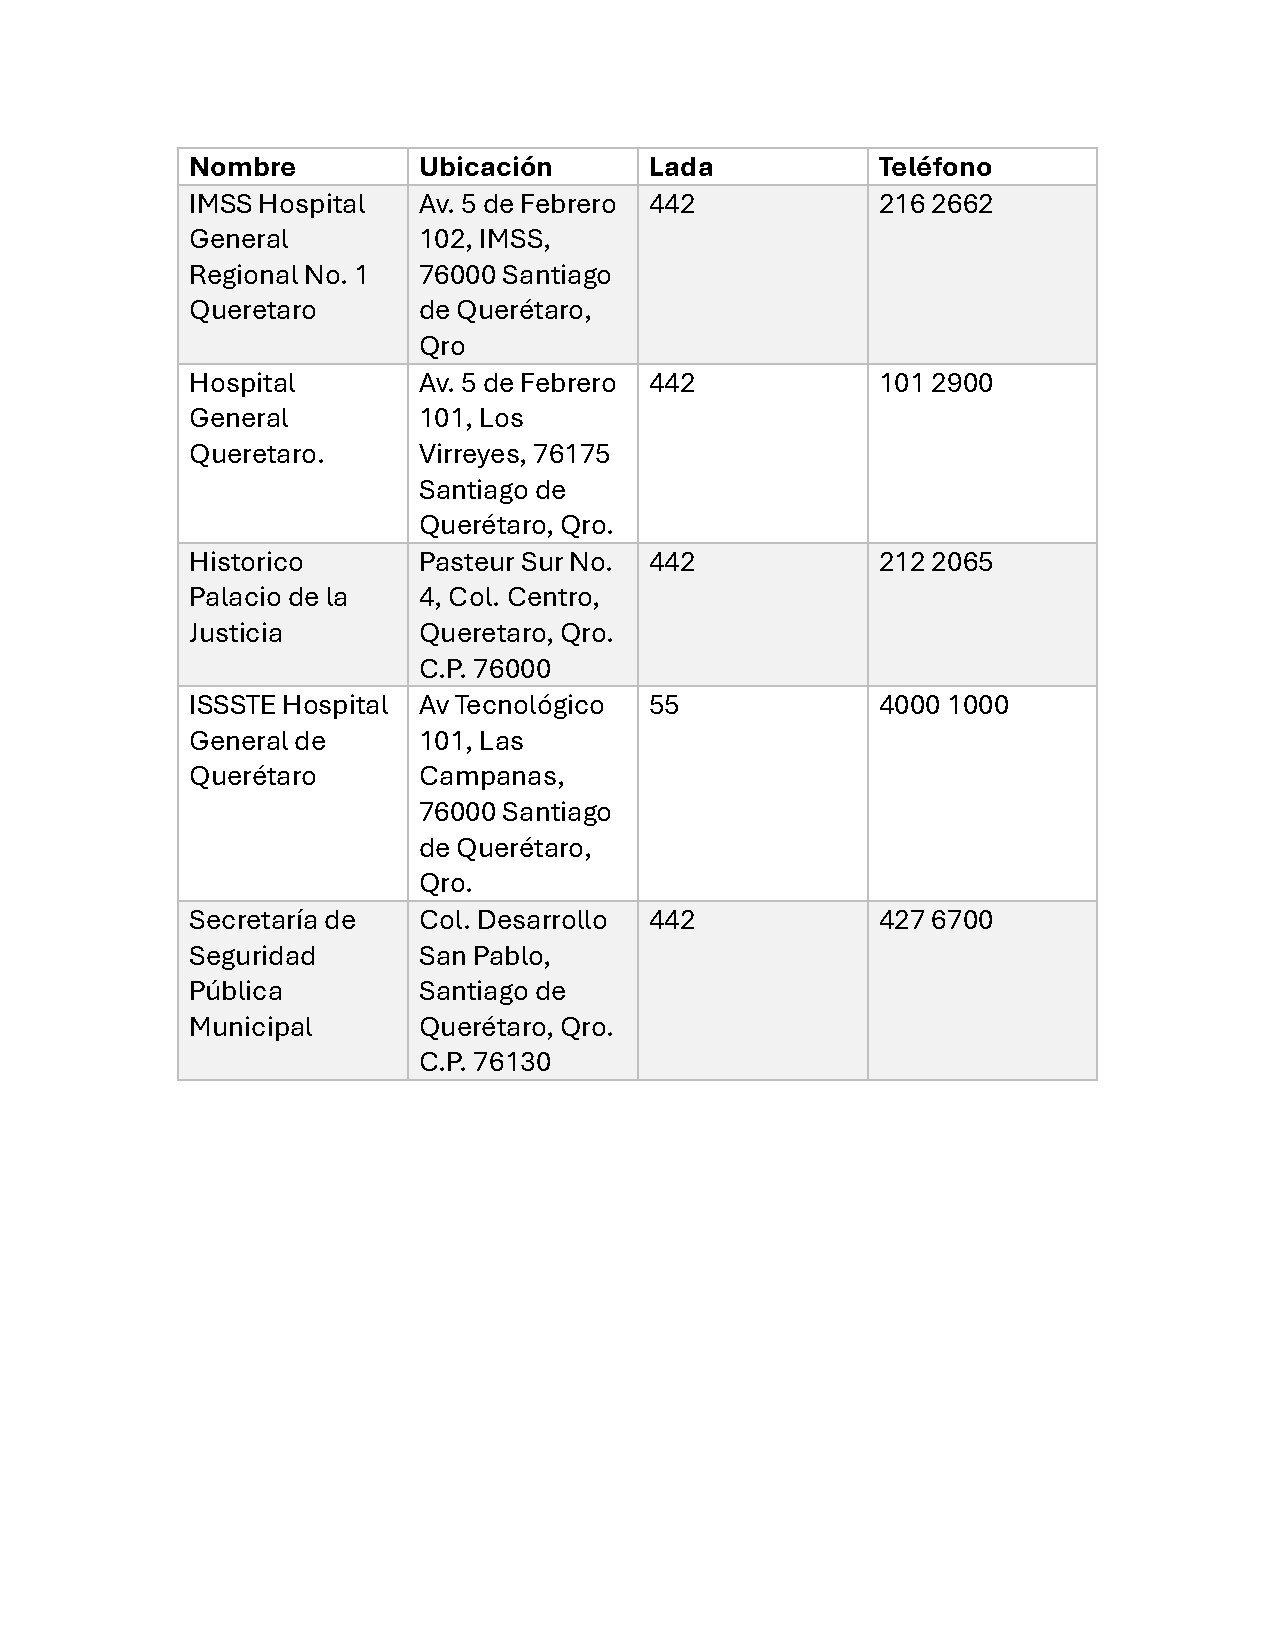
\includegraphics[scale=0.25]{13/img/apoyosExternos.pdf}
        \caption{Apoyos externos}
        \label{fig:Apoyos externos}
    \end{figure}
    % 
    %\begin{figure}[H]
      %  \centering
      %  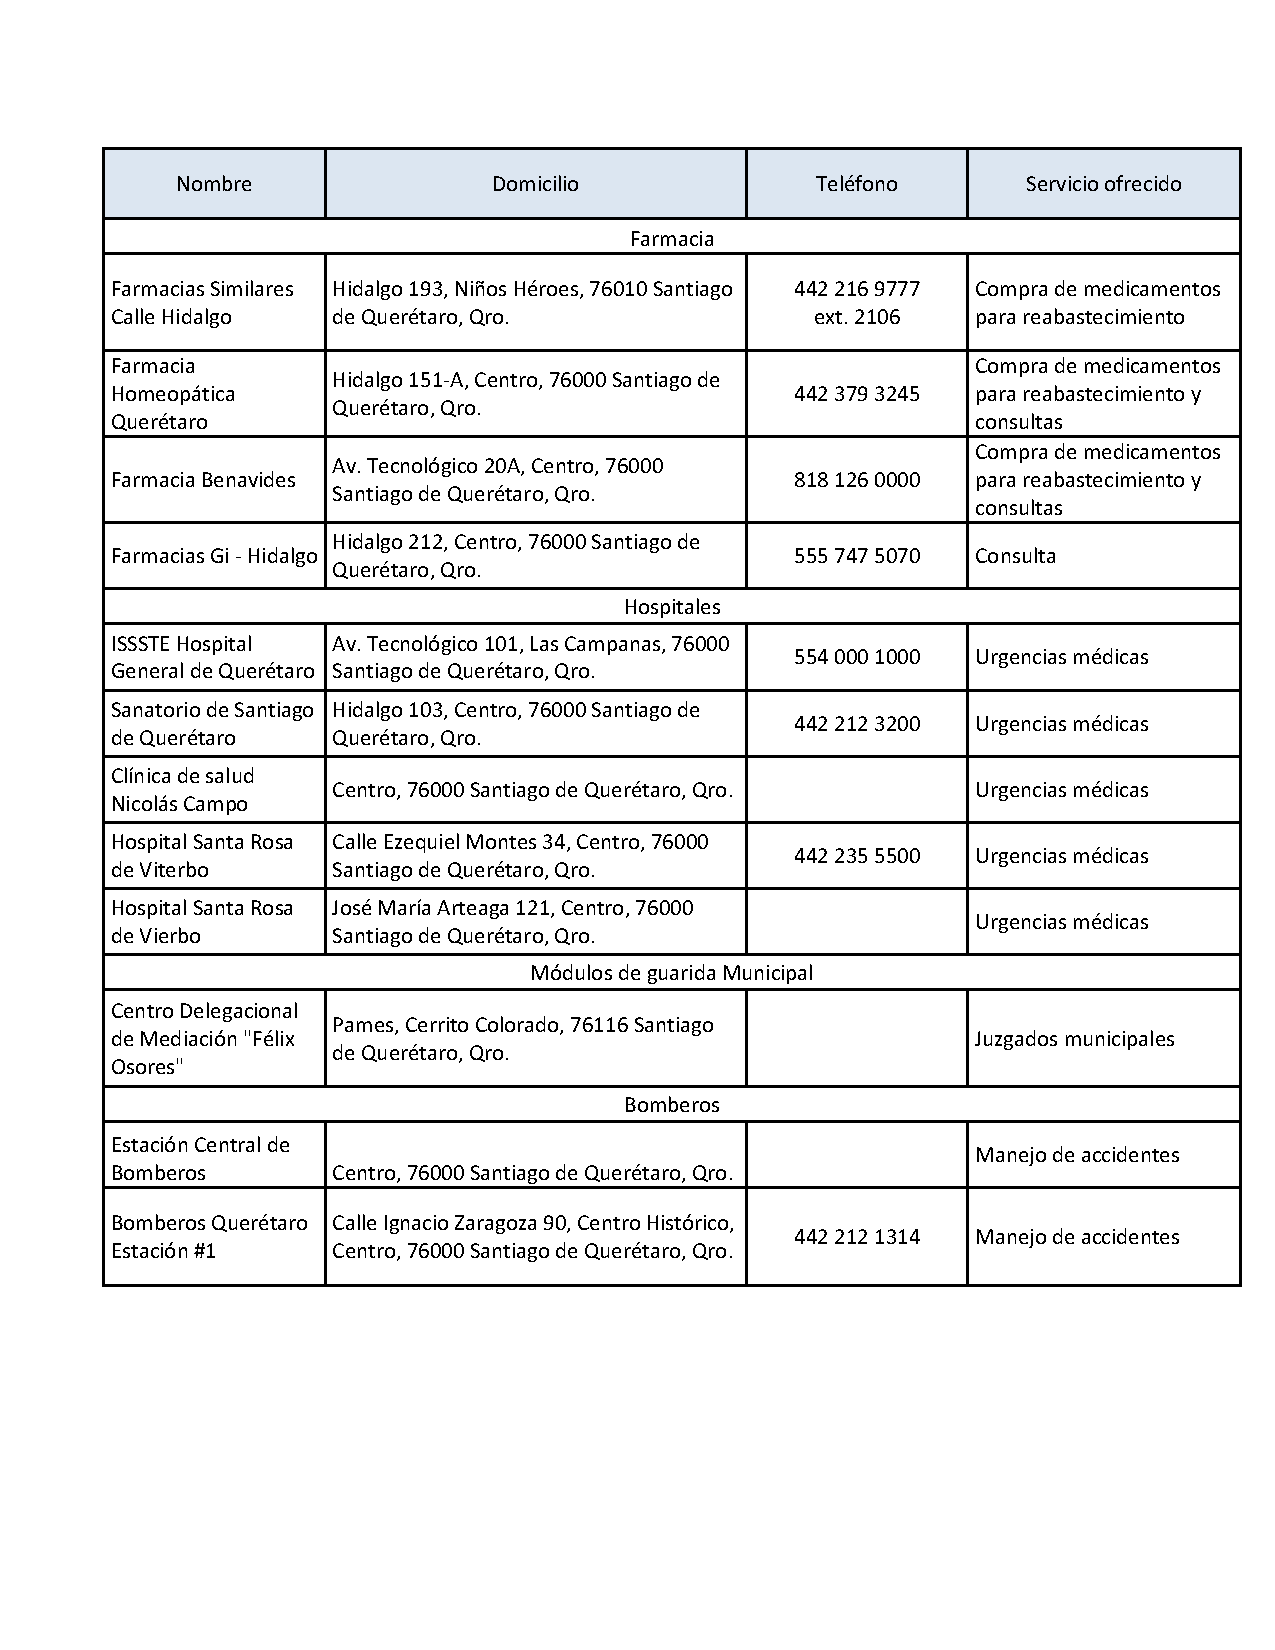
\includegraphics[trim = {20mm 95mm 20mm 41mm},clip,scale=0.5]{6/Img/apoyosExt.pdf}
       % \caption{ Lugares que servirán de apoyo en un situación de emergencia.}
       % \label{fig:apoyosExt}
    %\end{figure}
    % 
    % 
    \subsubsection{Identificación de puntos de reunión}
    \begin{figure}[H]
        \centering
        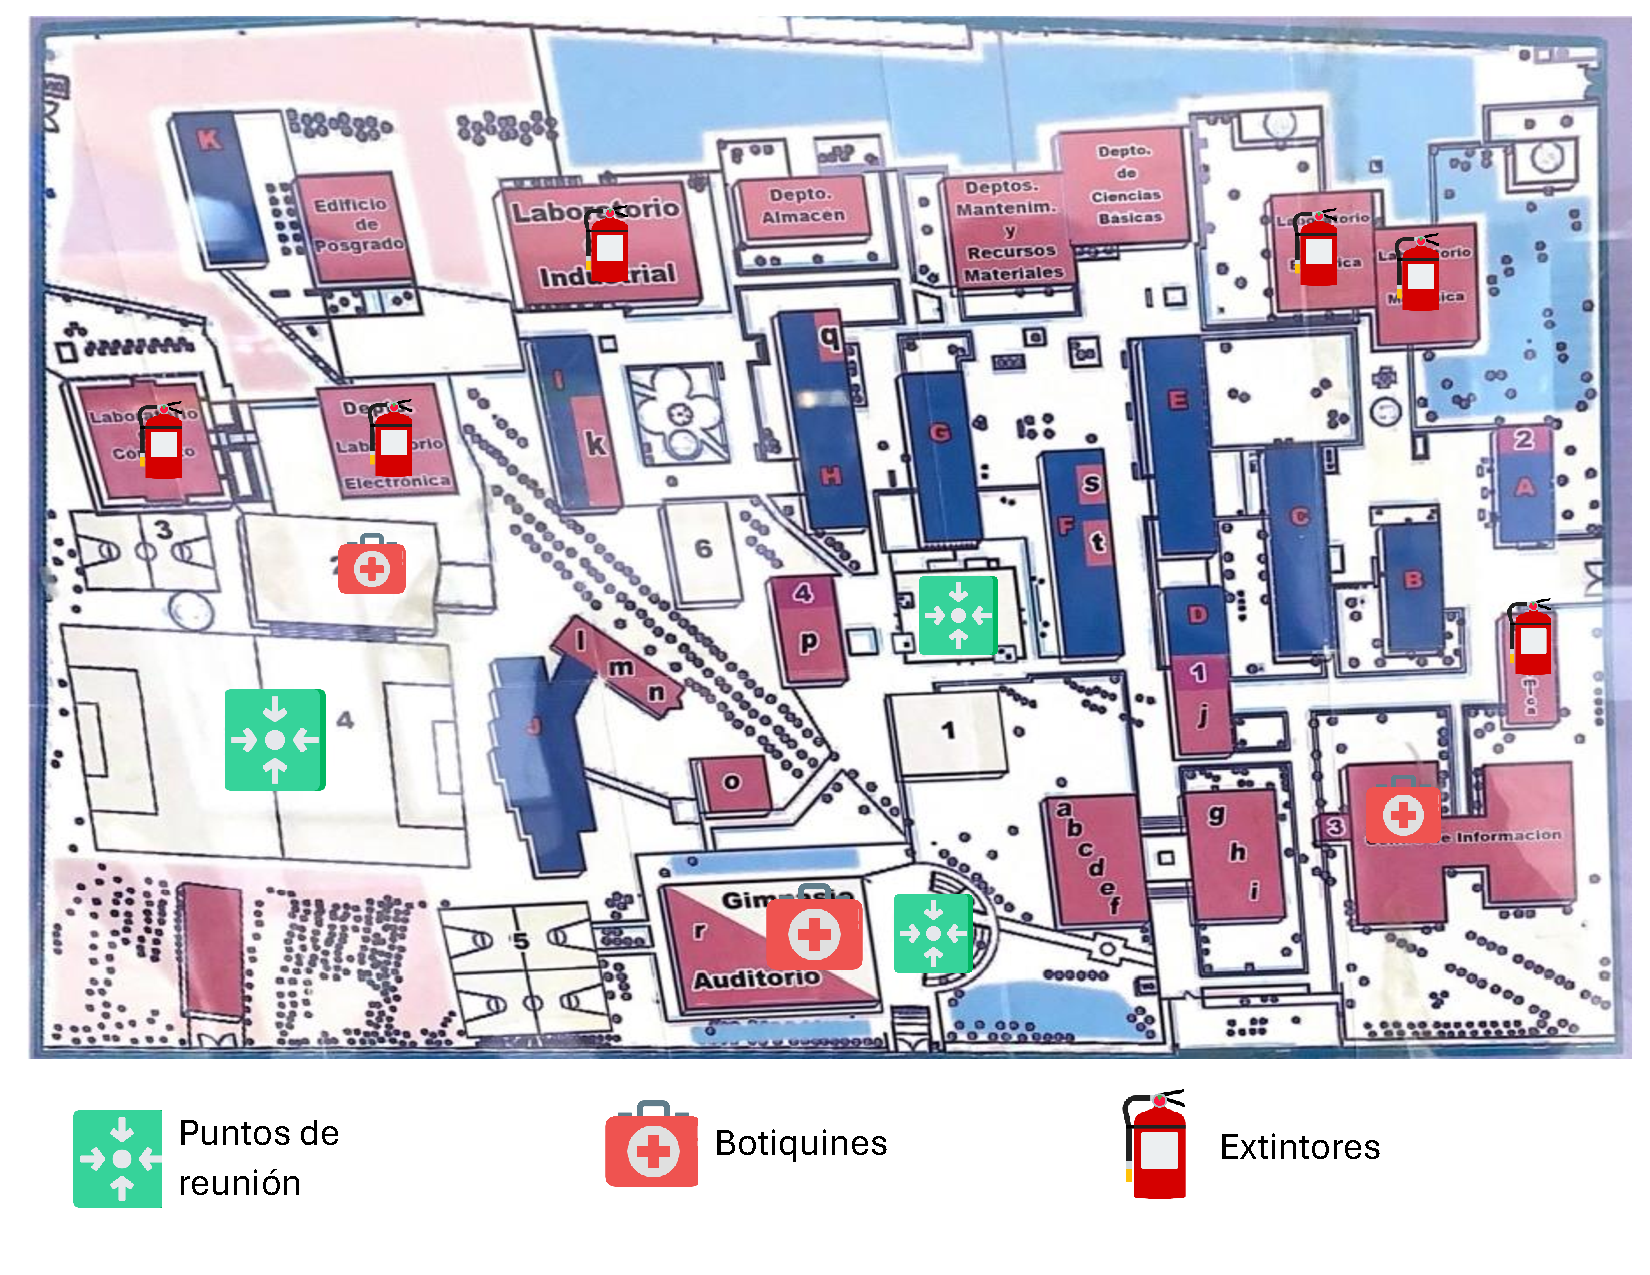
\includegraphics[scale=0.25]{13/img/localizacionDeRecursos.pdf}
        \caption{puntos de reunion}
        \label{fig:puntos de reunion}
    \end{figure}
    %\begin{figure}[H]
      %  \centering
       % \includegraphics[trim = {40mm 60mm 20mm 21mm},clip,scale=0.35]{6/Img/puntosDeReunión.pdf}
      %  \caption{Zona segura en caso de una evacuación de emergencia.}
      %  \label{fig:puntosDeReunión}
    %\end{figure}
    % 
    % 
    \subsubsection{Brigada de evacuación}
    \begin{figure}[H]
        \centering
        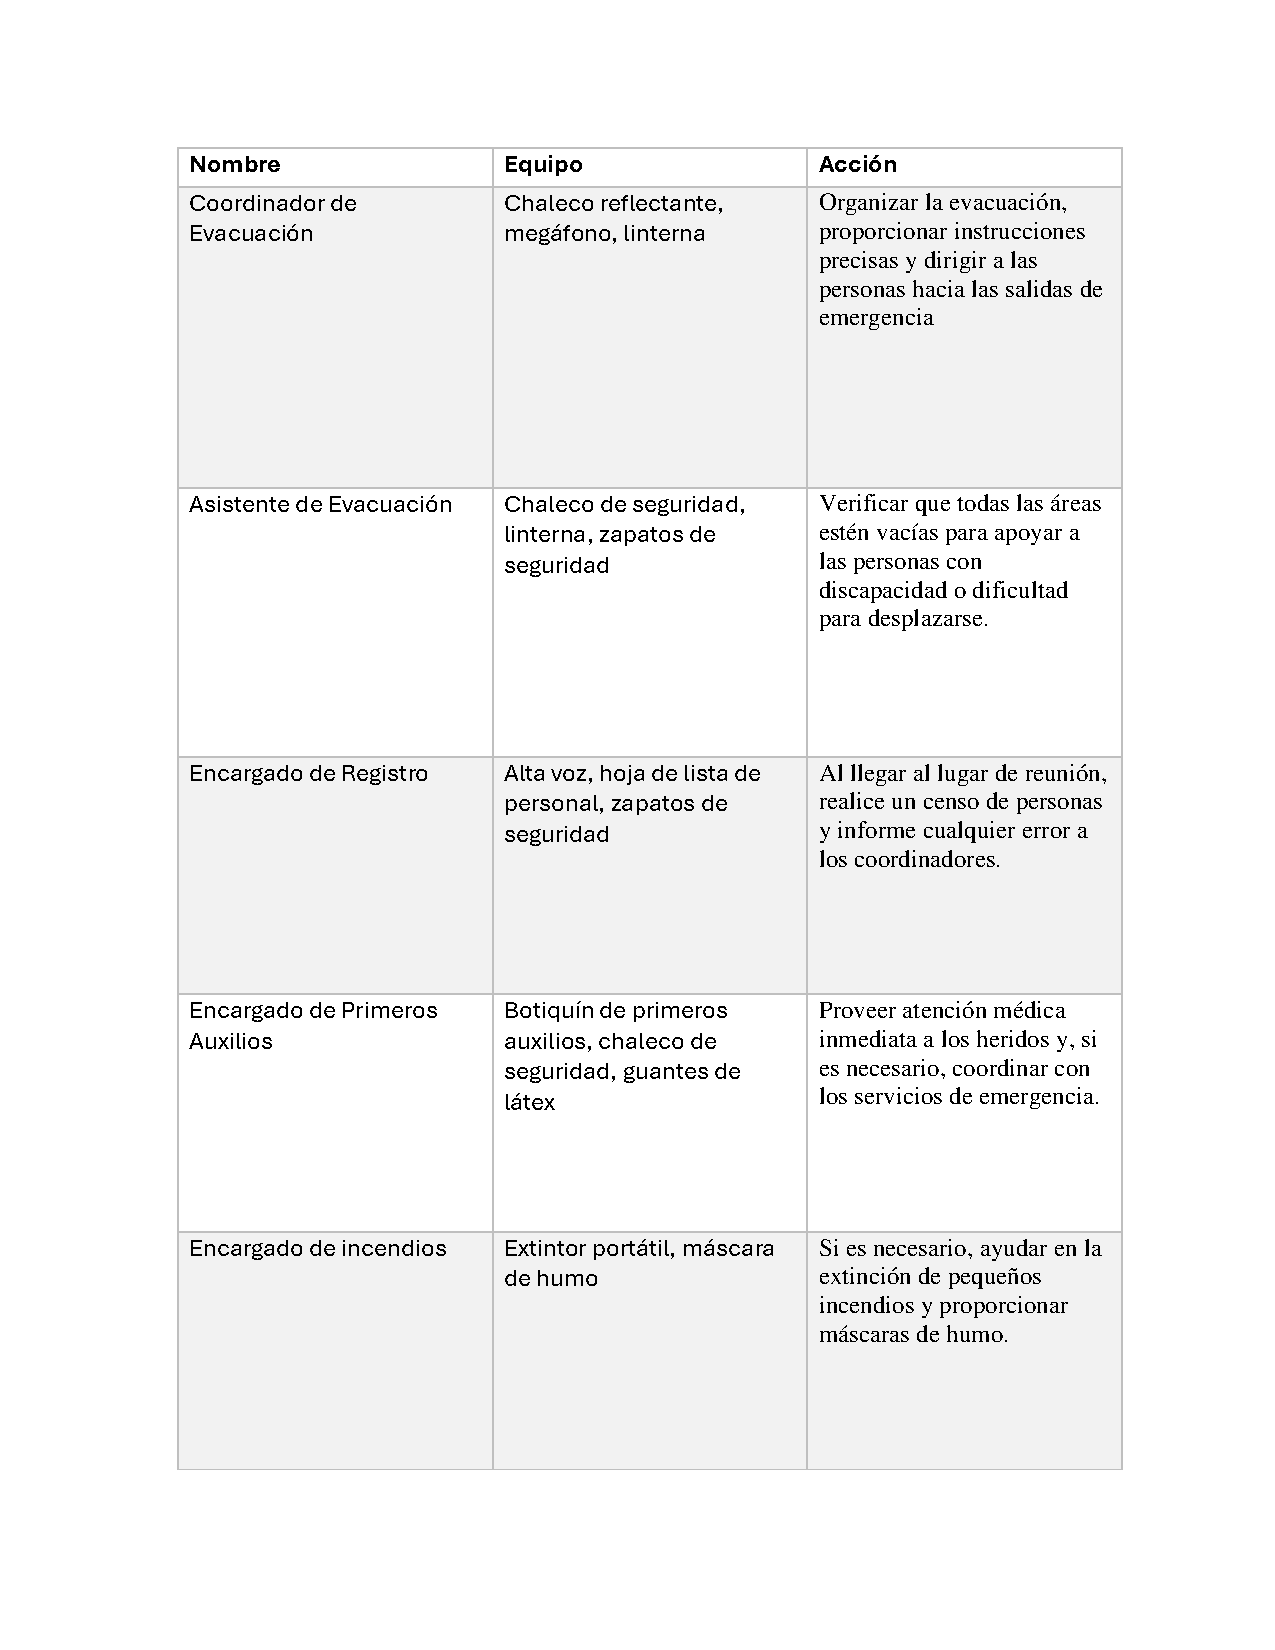
\includegraphics[scale=0.4]{13/img/brigada.pdf}
        \caption{Brigada de evacuación}
        % \label{fig:Brigada de evacuacion}
    \end{figure}
    %\begin{figure}[H]
       % \centering
      %  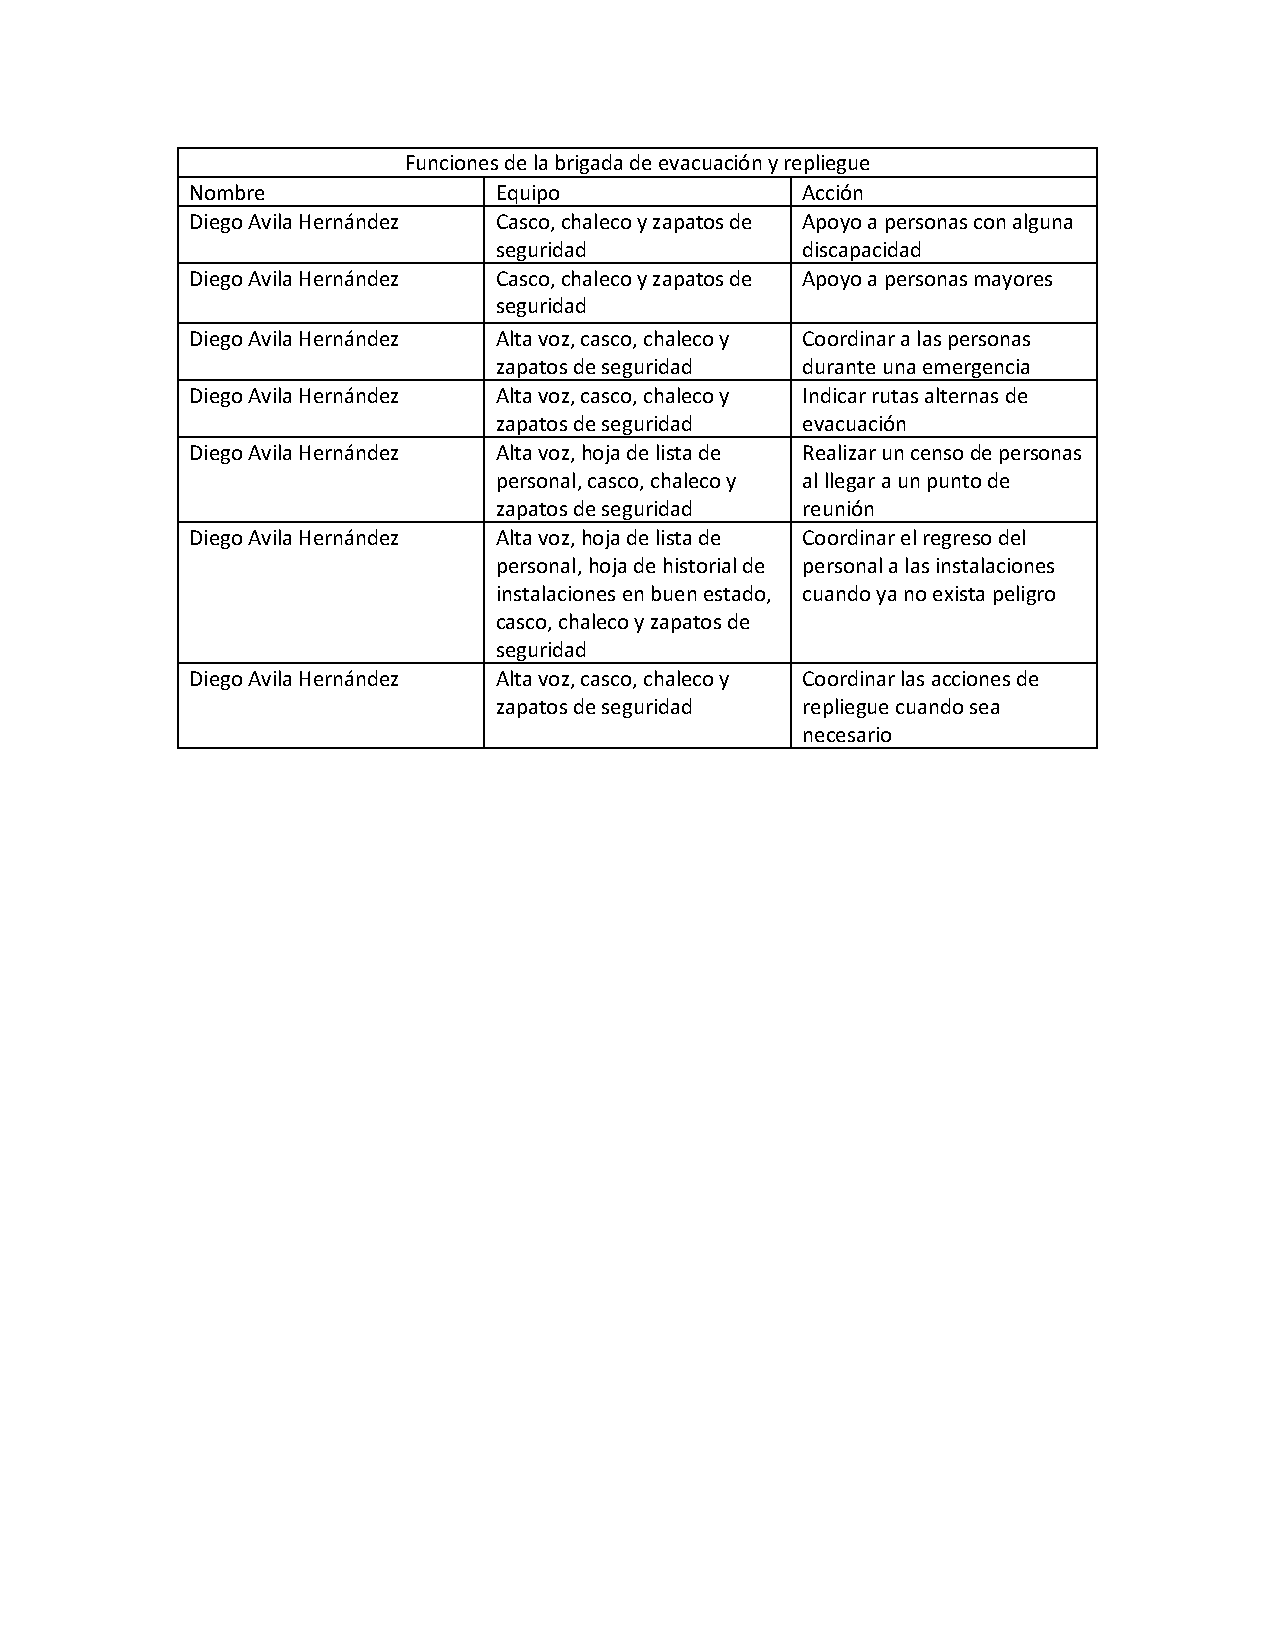
\includegraphics[trim = {20mm 90mm 40mm 45mm},clip,scale=0.5]{6/Img/brigada.pdf}
       % \caption{Acciones asignadas a cada integrante del equipo de trabajo en caso de una evacuación de emergencia o repliegue.}
       % \label{fig:brigada}
    %\end{figure}
    % 
    % 
    \subsubsection{Directorio de telefónicos de emergencia}
    
    Un Directorio Telefónico de Emergencia es una lista ordenada de números de teléfono de contactos importantes que pueden ser necesarios en situaciones de emergencia. 
    \subsubsection{Brigada de evacuación}
    \begin{figure}[H]
        \centering
        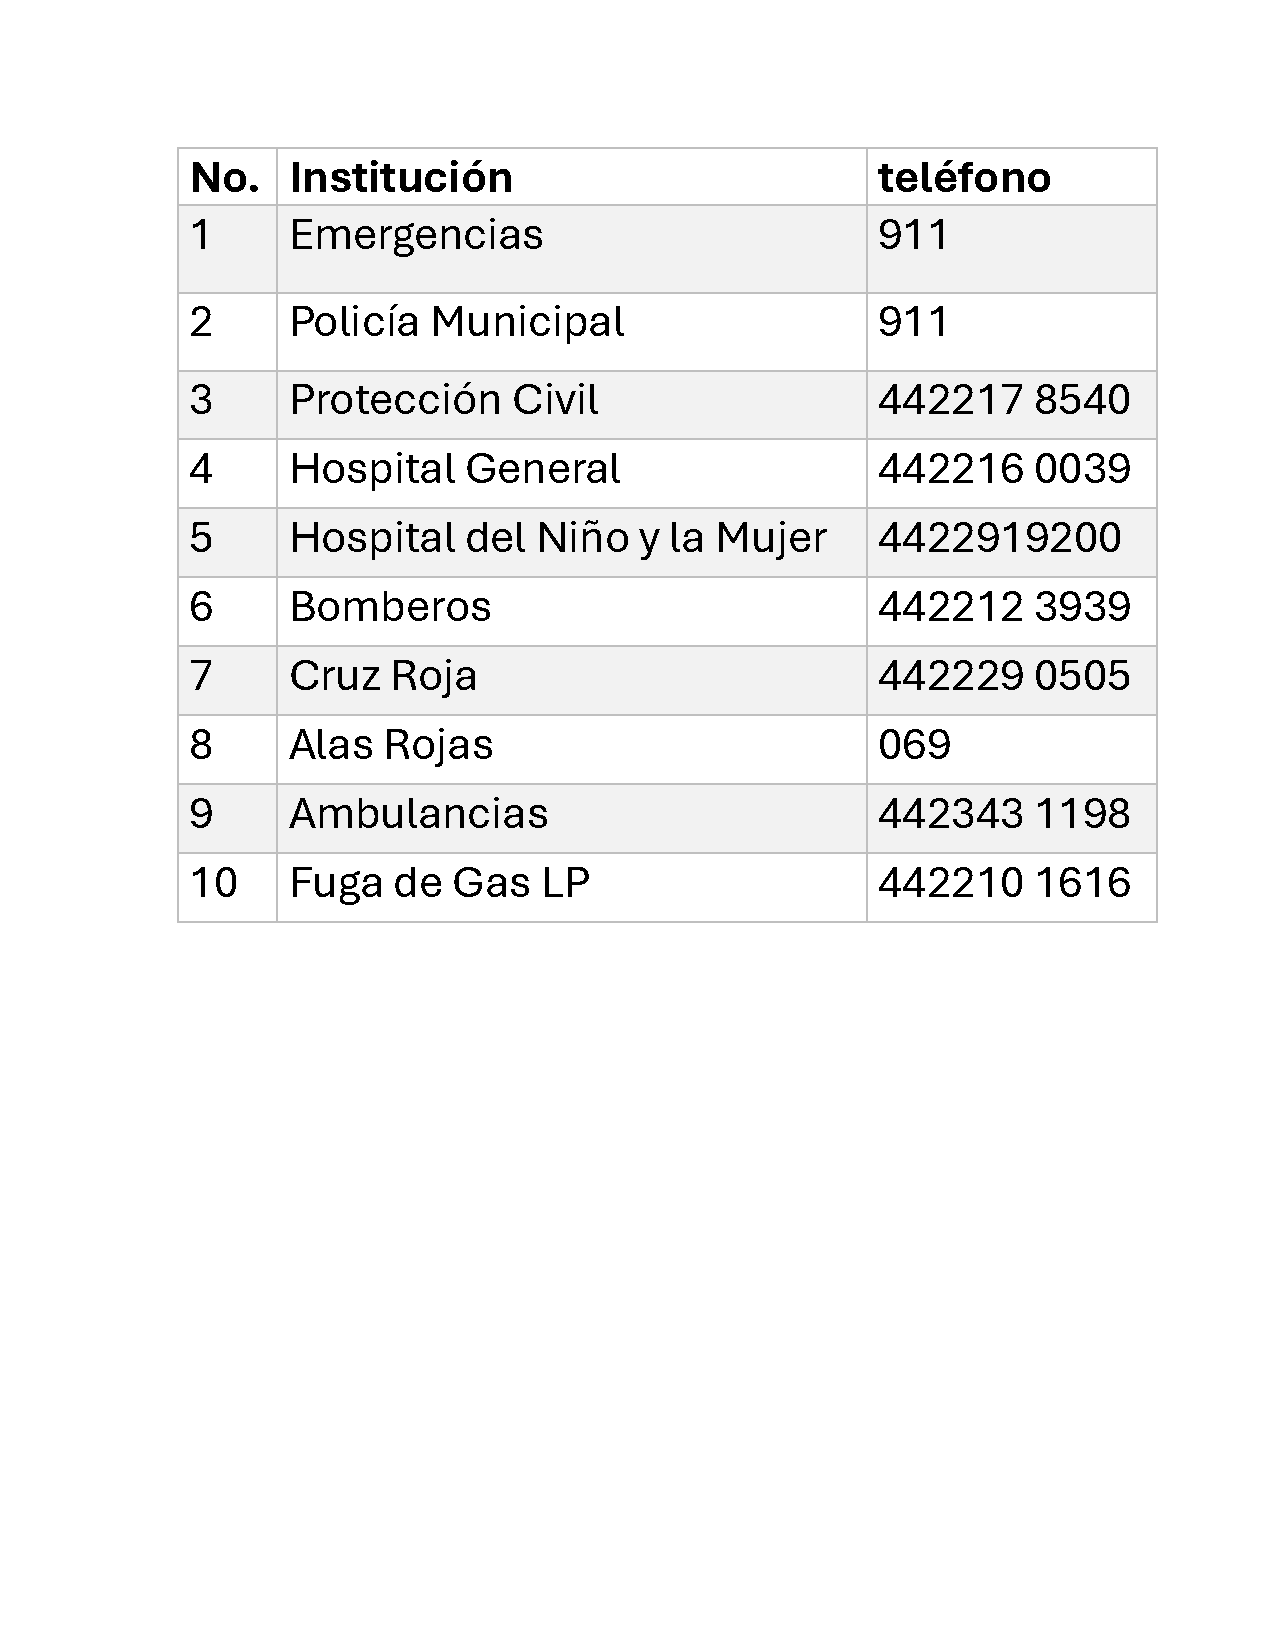
\includegraphics[scale=0.4]{13/img/directrorio.pdf}
        \caption{Directorio de telefónicos de emergencia}
        % \label{fig:Directorio de telefonicos de emergencia}
    \end{figure}
    
    %\begin{figure}[H]
       % \centering
       % 
\includegraphics[scale=0.25]{6/Img/911.PNG}
        %\caption{Números de emergencia de los bomberos más próximos a la ubicación el posible riesgo}
    %\end{figure}
    % 
    % 
    %\begin{figure}[H]
       % \centering
        %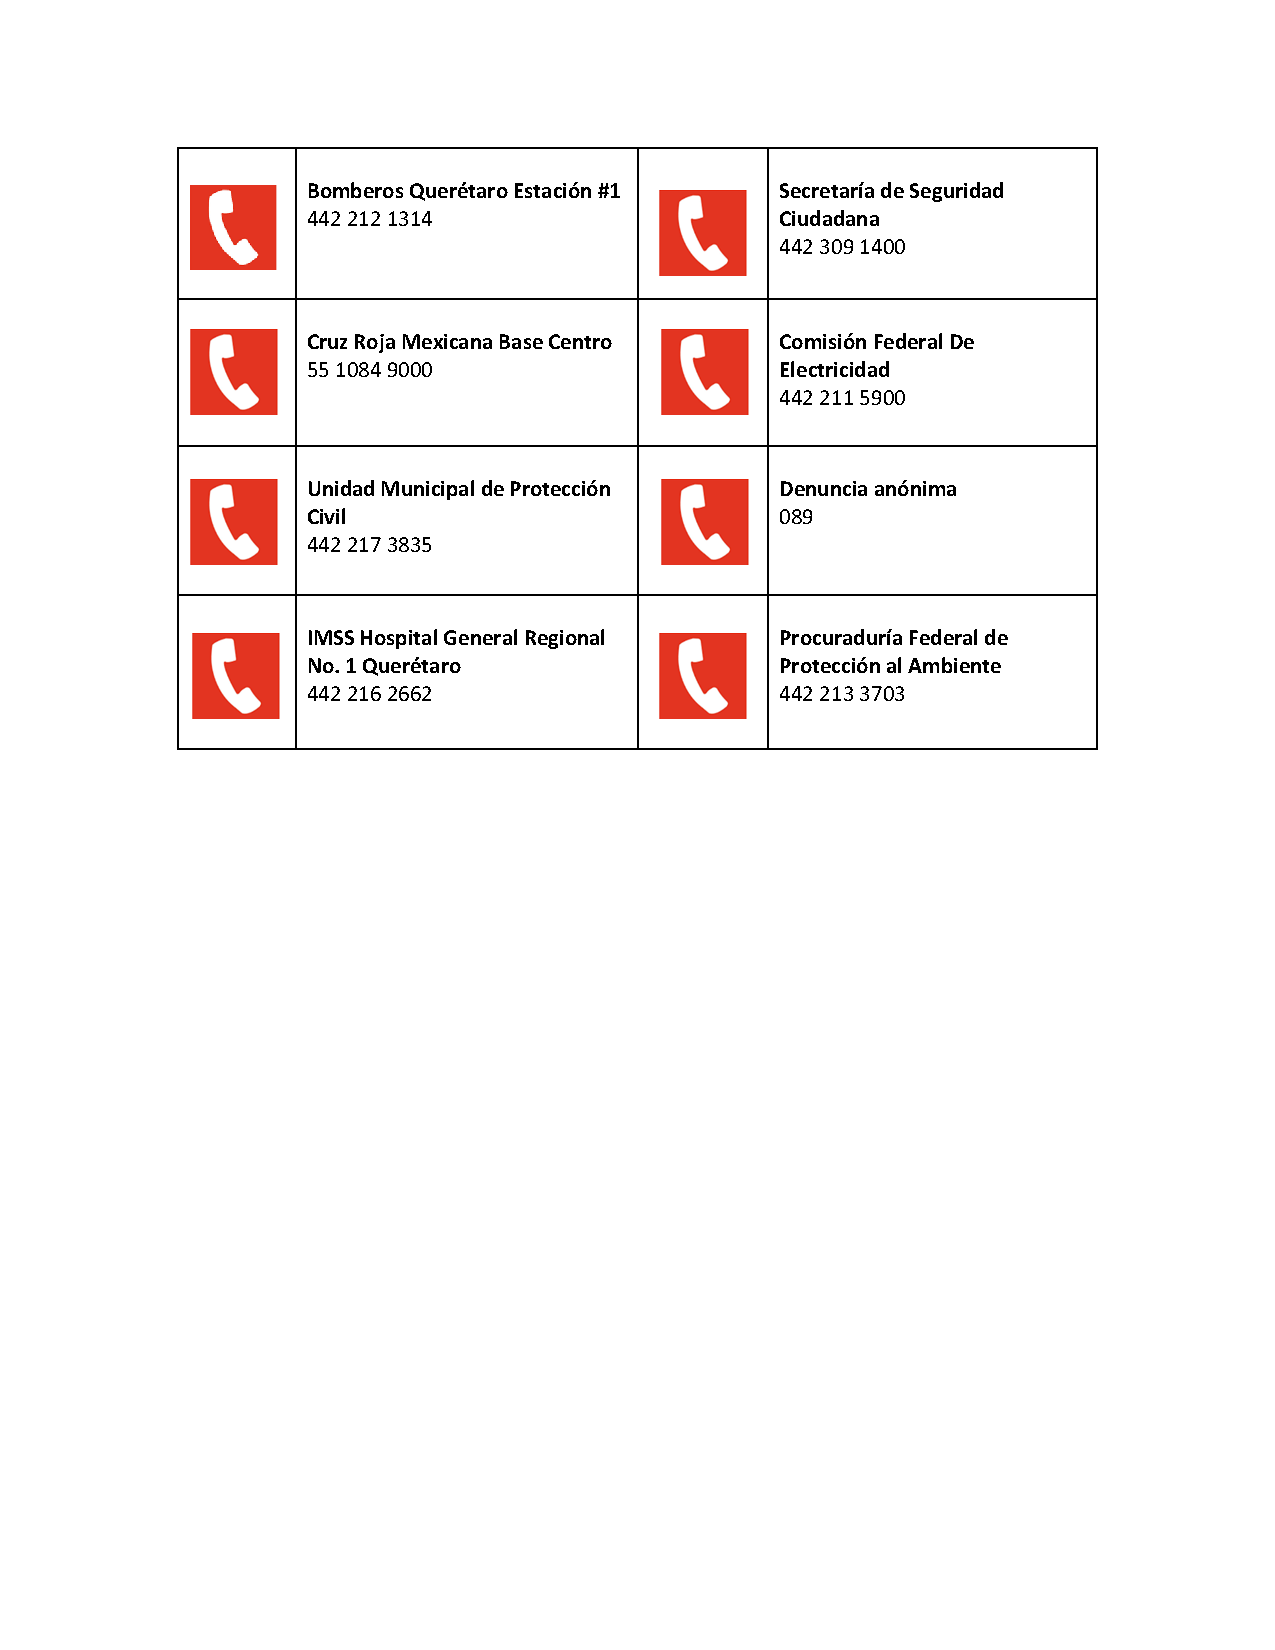
\includegraphics[scale=0.45]{6/Img/directorio.PNG}
        %\caption{Números de emergencia de los bomberos más próximos a la ubicación el posible riesgo}
    %\end{figure}
    % 
    % 
    \subsection{Análisis de los métodos, materiales, herramientas e instalación utilizada en la ejecución del ensamble de un circuito electrónico}
    
    \subsubsection{Verificación}
    
    Costos de no calidad.
    % 
    % 
    \subsubsection{Desarrollo del sistema de tiempos predeterminado}
    % 
    \begin{figure}[H]
        \centering
        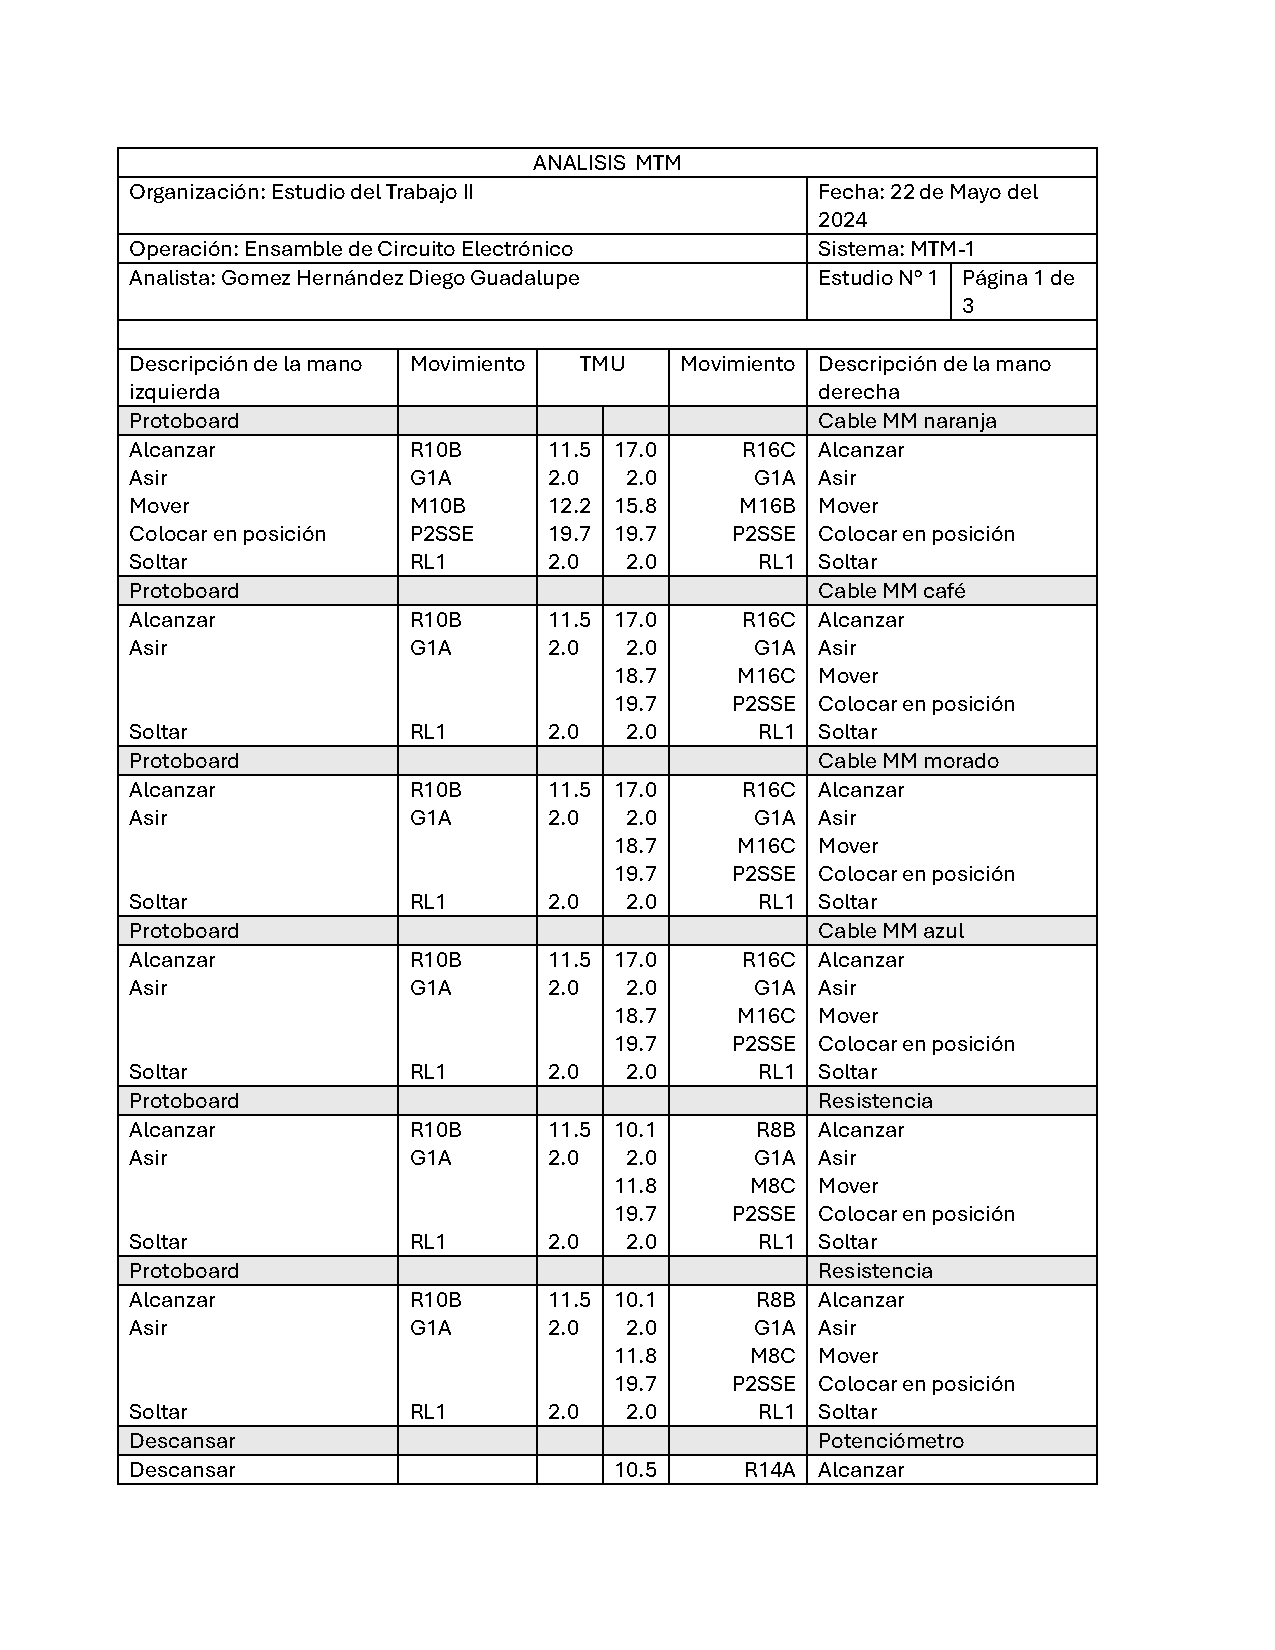
\includegraphics[scale=0.21]{13/img/analisMtmUno.pdf}
        \centering
        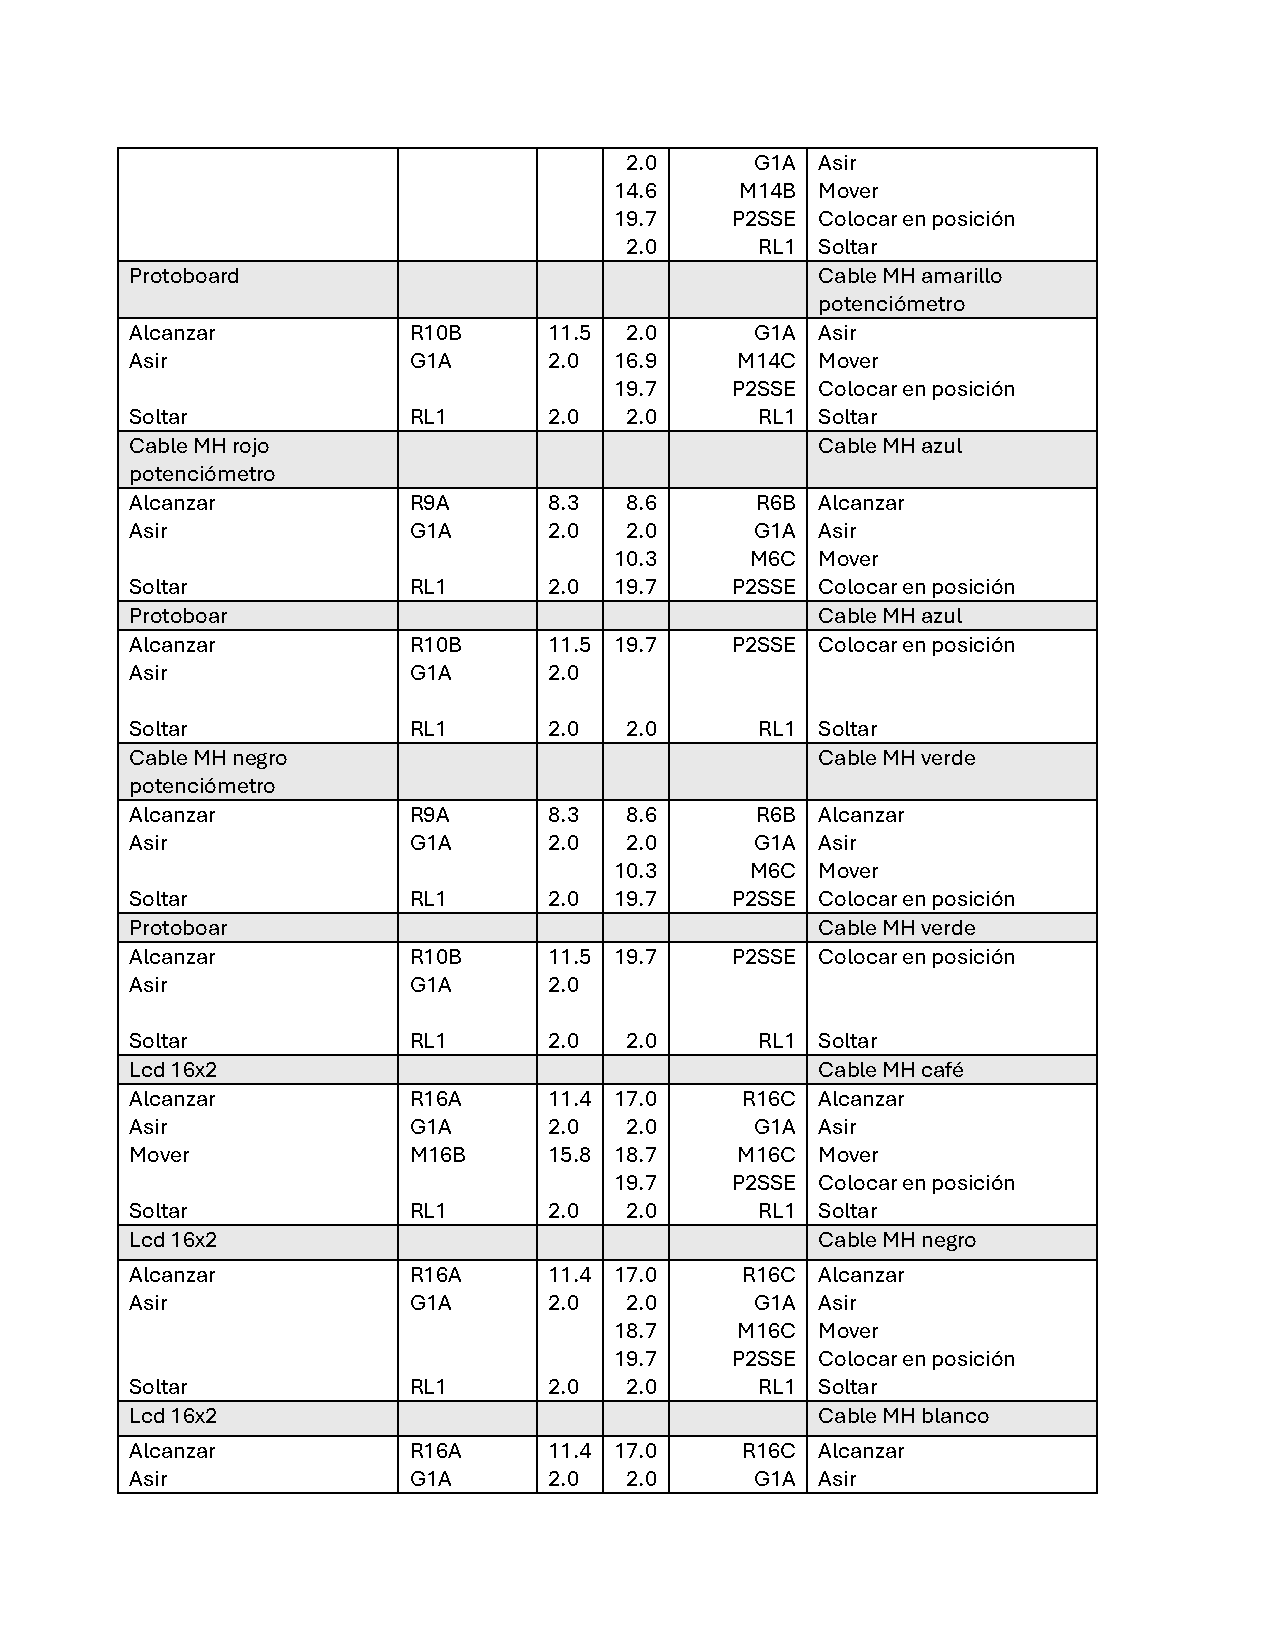
\includegraphics[scale=0.21]{13/img/analisMtmDos.pdf}
        \centering
        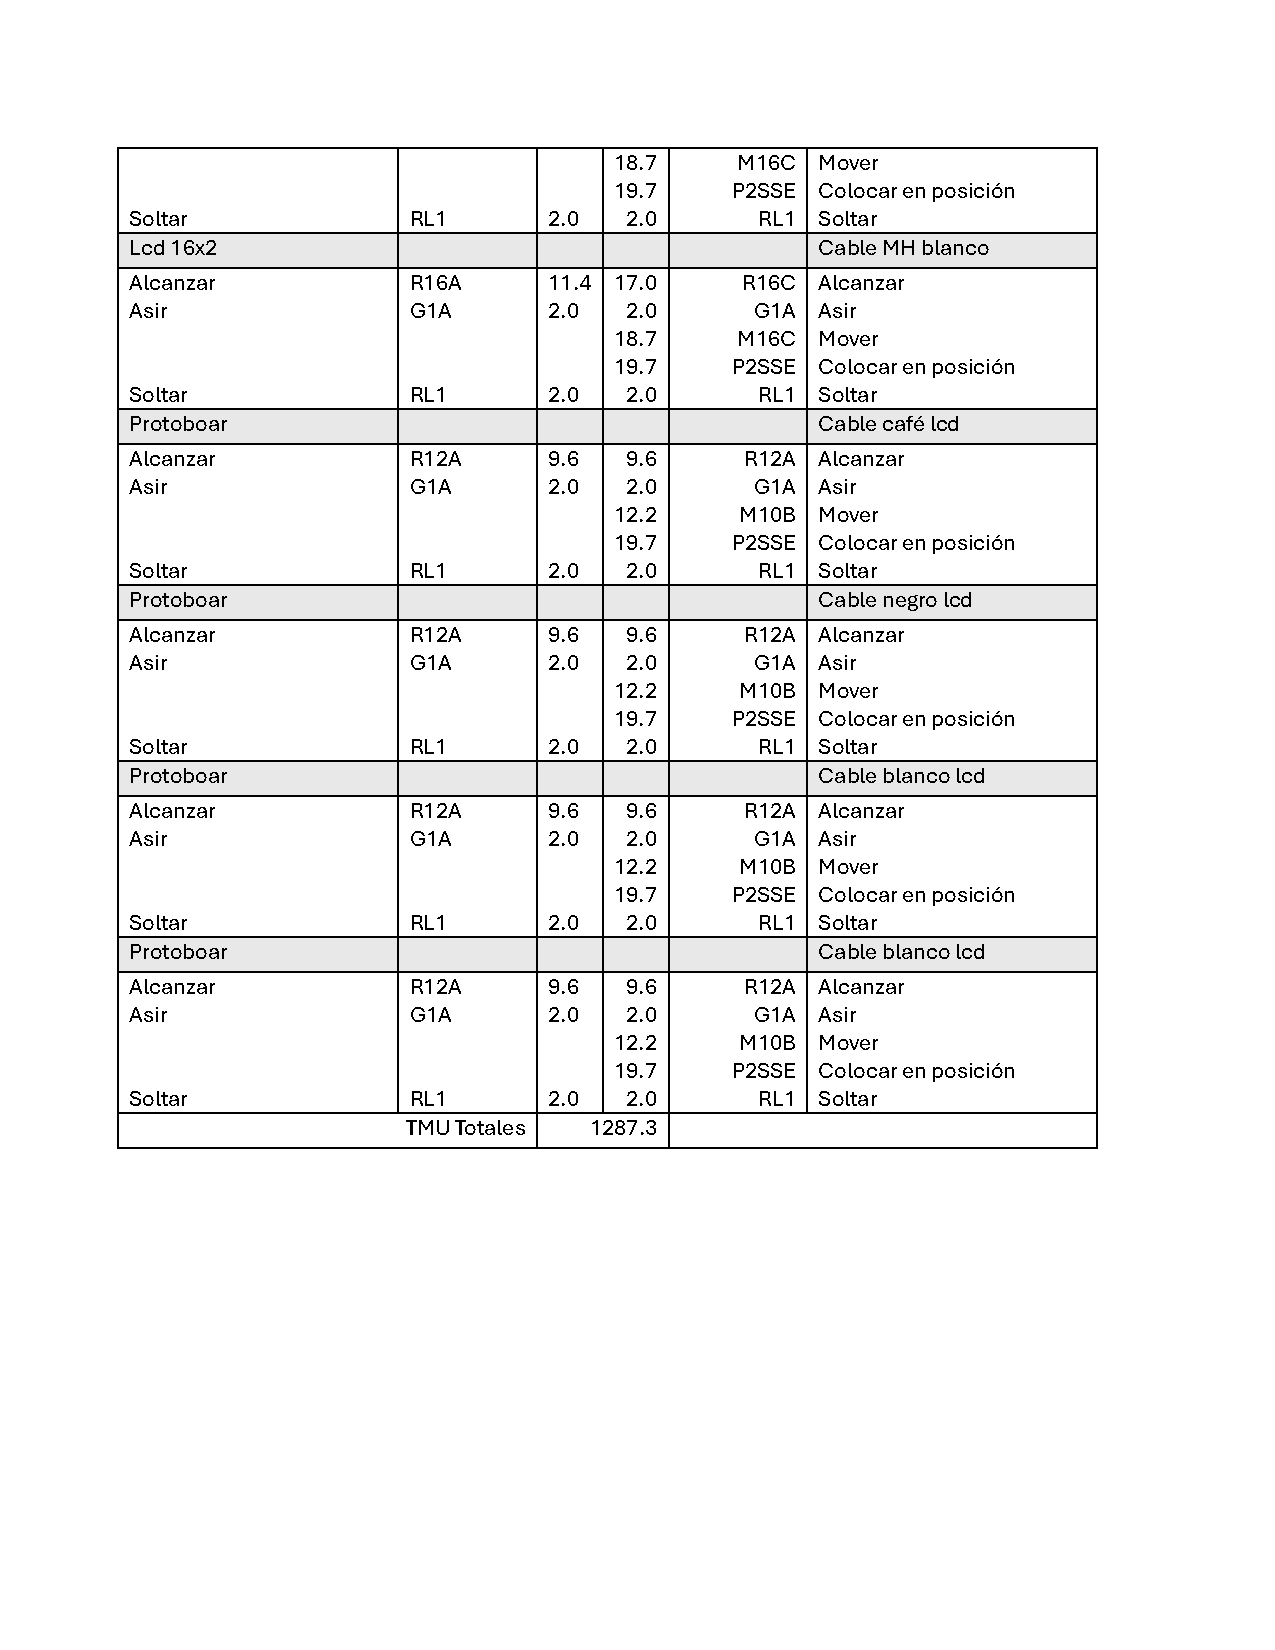
\includegraphics[scale=0.21]{13/img/analisMtmTres.pdf}
        \caption{analisis Mtm}
        \label{fig:analisis Mtm}
    \end{figure}
    % 
    \subsubsection{Desarrollo del muestreo del trabajo}
    % 
    \begin{figure}[H]
        \centering
        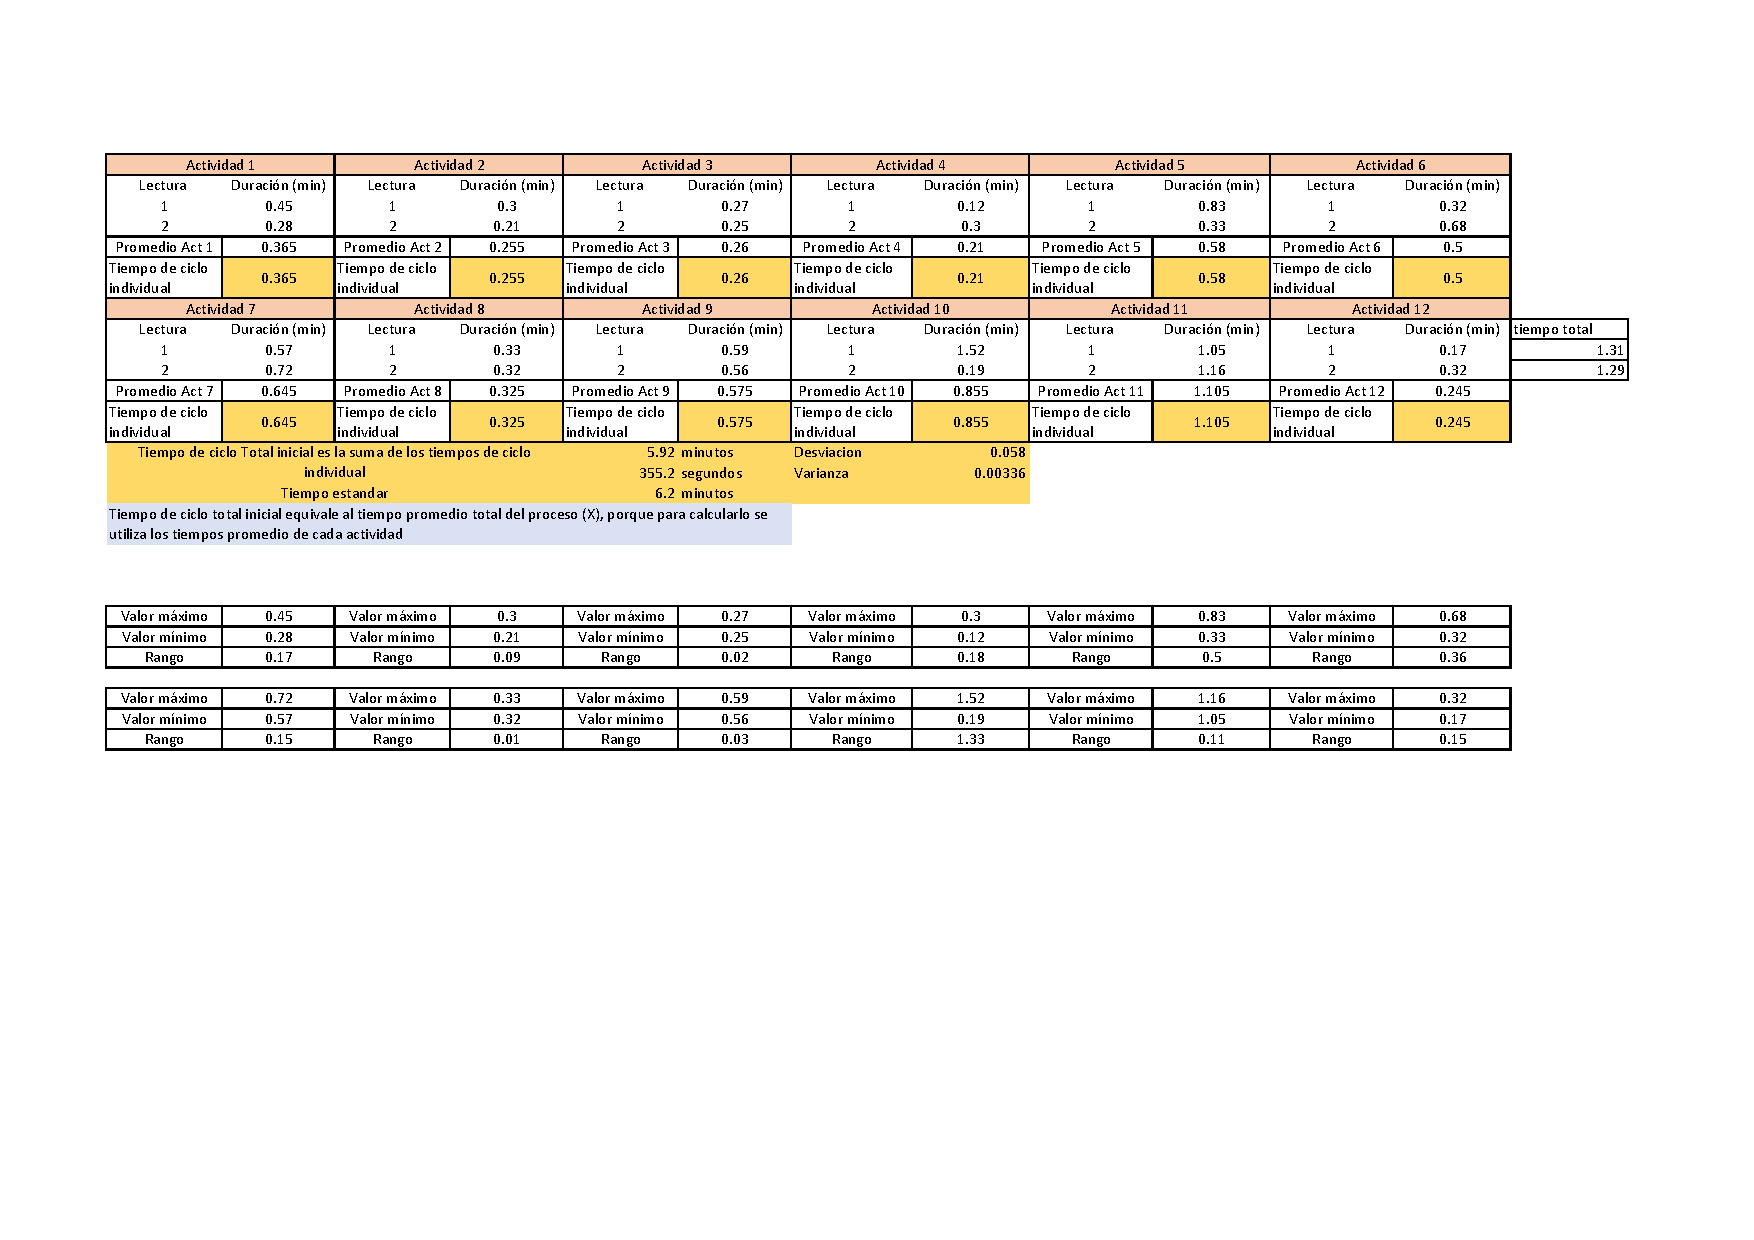
\includegraphics[scale=0.25]{13/img/tiempoCicloEnsamble.pdf}
        \caption{Tiempo ciclo}
        \label{fig:Tiempo ciclo}
    \end{figure}
    \begin{figure}[H]
        \centering
        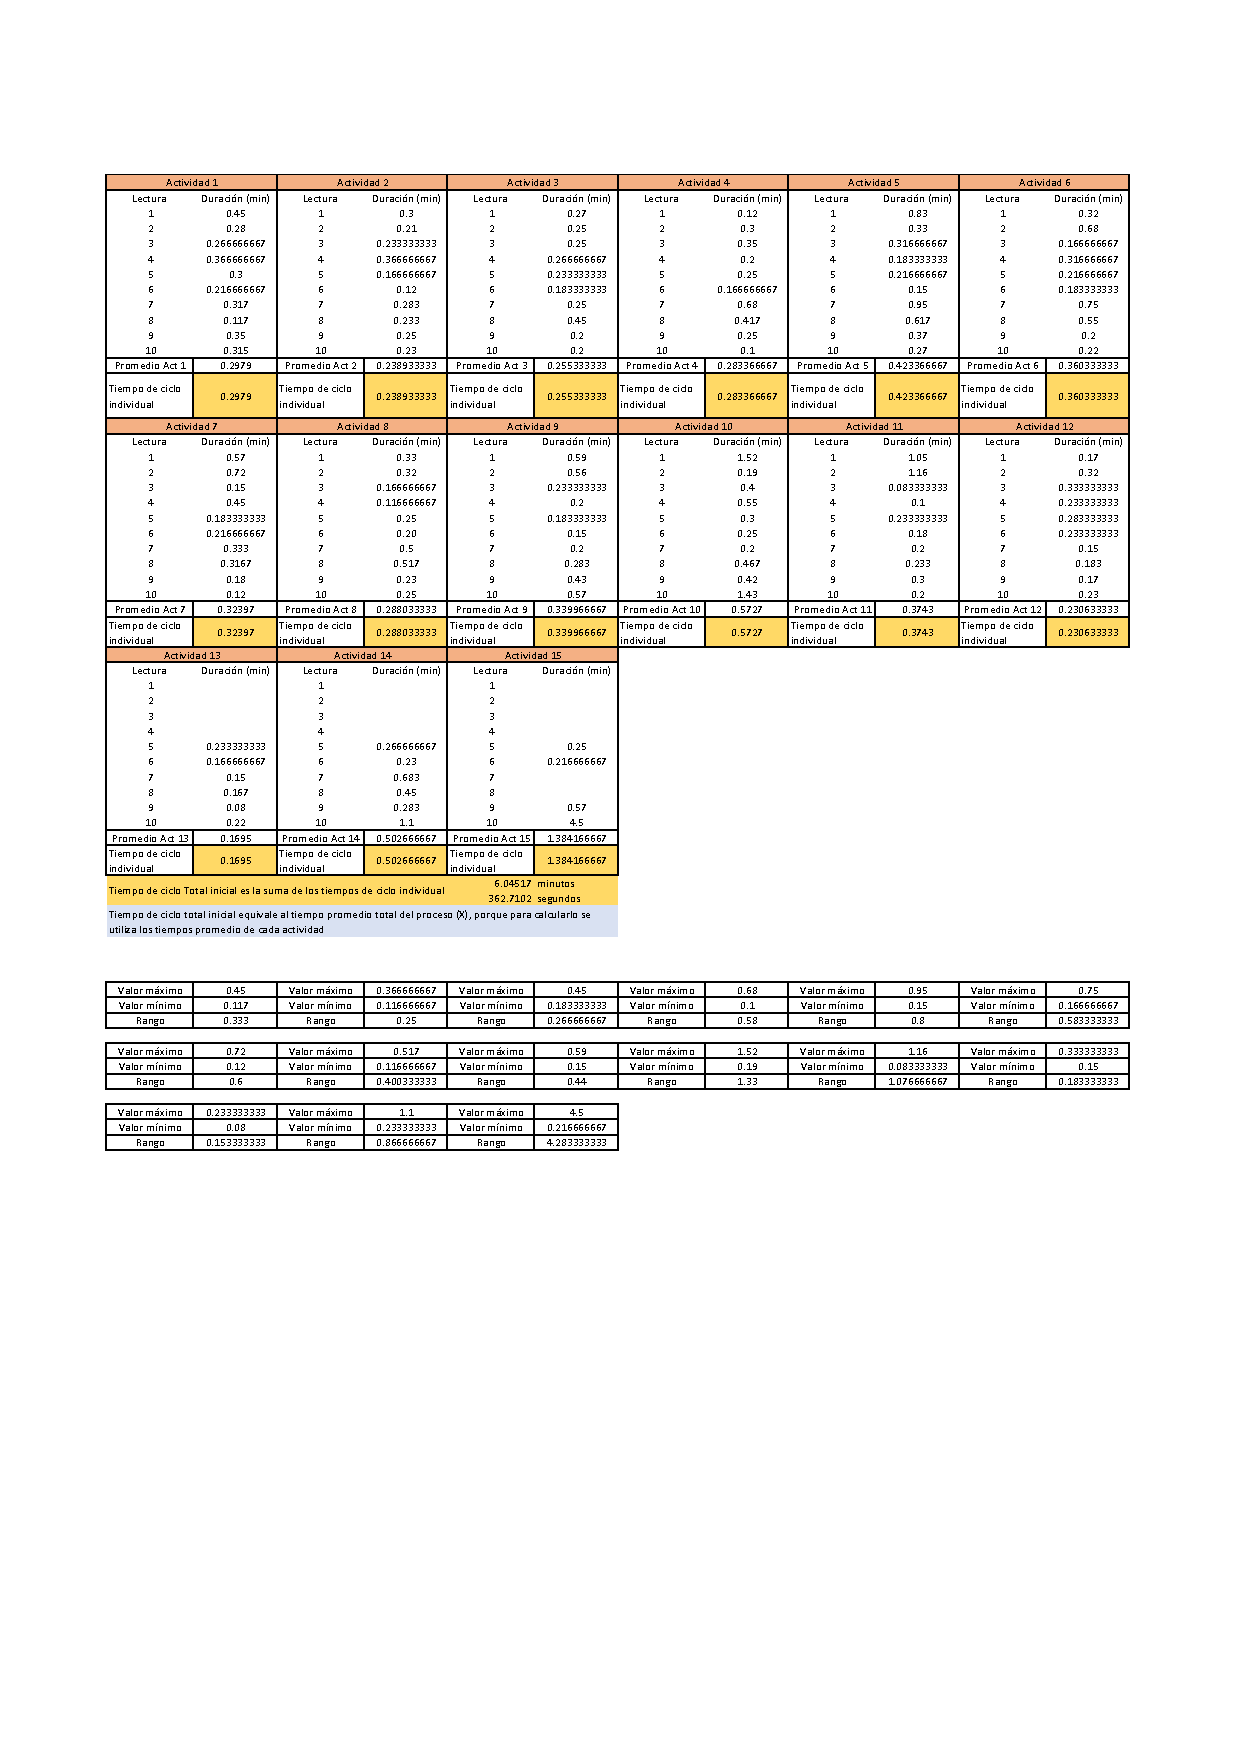
\includegraphics[scale=0.25]{13/img/tiempoCicloEnsambleDos.pdf}
        \caption{Muestreo}
        \label{fig:Muestreo}
    \end{figure}
    % 
    \subsubsection{Corrección por balanceo de procesos}
    % 
    % 
    \subsubsection{Datos estándar continuos y discretos}
    % 
    % 
    \subsection{Diseño de la forma más económica de realizar el trabajo}
    
    % 
    % 
    \subsection{Normalización de los métodos, materiales, herramientas e instalaciones}
    
    % 
    % 
    \subsection{Determinación del tiempo estándar para que una persona competente realice el trabajo con marcha normal}
    
    
    % 
    % 
    \section{Conclusiones}
    
    Con el muestreo realizado logramos obtener distintas muestras las cuales nos sirvieron de ayuda para determinar nuestro tiempo estándar y poder saber quién era el operador promedio y cuál era el operador más lento para posteriormente realizar un balanceo de líneas y poder reducir nuestros tiempos con ayuda de los therblings logrando así que nuestros costos de operación se reduzcan logrando obtener una producción balanceada y con un costo de producción bajo con esto cumplimos la etapa del estudio de movimientos y tiempos la cual dice que debemos encontrar la forma más económica de hacer el trabajo.Se logro establecer un tiempo estándar de  6 minutos para el ensamble aplicando los STP y el uso de probabilidades. 
    Con todo lo planteado y que se realizo en este proyecto podemos concluir de que se lograron los objetivos dejándonos varias habilidades nuevas las cuales se implementaras en distintos proyectos.
    
    \section{Agradecimientos}
    
    Es importante darles su debido reconocimiento a los laboratorios, instituciones, organizaciones, entre otros que han sido participes para la culminación de este trabajo. También es importante mencionar, fondos, proyectos, becas, entre otros que se le han otorgado al o los autores para realizar el trabajo de investigación. Ejemplo: “Los autores agradecen al Concejo Nacional de Ciencia y Tecnología por los recursos otorgados…”
    
    %\section*{Referencias}
    
    %Para esta platilla, se solicita al autor enumerar las citas de manera consecutiva entre corchetes . 
    %La puntuación de la oración que sigues sería . 
    %Refiérase simplemente al número de referencia, como en , no utilice “Ref. [3]” o “referencia [3]” excepto al principio de una oración: “La referencia [3] fue la primera…”
    %Enumere las notas al pie por separado en superíndices. Coloque la nota de pie de en la parte inferior de la columna en la que se citó. No coloque notas al pie en la lista de referencias. Utilice letras para las notas al pie de la tabla.
    %A menos de que haya tres autores o más; no utilice “et al.”. Los trabajos que no hayan sido publicados, incluso si han sido presentados para su publicación, deben ser citados como “inéditos”. Los trabajos que han sido aceptados para su publicación deben de citarse como “en prensa”. Poner en mayúscula sólo la primera palabra de un título, excepto los nombres propios y los símbolos de elemento. 
    
    
    % Ejemplo
    %  @Article{article,
    % 	author = "Author1 LastName1 and Author2 LastName2 and Author3 LastName3",
    % 	title = "Article Title",
    % 	volume = "30",
    % 	number = "30",
    % 	pages = "10127-10134",
    % 	year = "2013",
    % 	doi = "10.3389/fnins.2013.12345",
    % 	URL = "http://www.frontiersin.org/Journal/10.3389/fnins.2013.12345/abstract",
    % 	journal = "Frontiers in Neuroscience"
    % }
    
    % @book{book,
    %   author    = {Author Name}, 
    %   title     = {The title of the work},
    %   publisher = {The name of the publisher},
    %   address   = {The city},
    %   year      = 1993,
    % }
    
    % @incollection{chapter,
    %   author       = {Bauthor Surname}, 
    %   title        = {The title of the work},
    %   editor       = {Editor Name},
    %   booktitle    = {The title of the book},
    %   publisher    = {The name of the publisher},
    %   address      = {The city},
    %   year         = 2002,
    %   pages        = {201-213},
    % }
    
    % @InProceedings{conference,
    %   author = {Cauthor Name and Dauthor Surname and Fauthor LastName},
    %   title = {The title of the work},
    %   booktitle = {The title of the conference proceedings},
    %   year = 1996,
    %   publisher = {The name of the publisher},
    %   editor = {Editor Name1 and Editor Name2},
    %   pages = {41-50},
    % }
    
    % @book{cho,
    %   author       = {Gauthor Name1}, 
    %   title        = {The title of the work},
    %   publisher = {Country code and patent number},
    %   address      = {Patent Country},
    %   year = 2013
    % }
    
    % @book{patent,
    %   author    = {Hauthor Surname1}, 
    %   title     = {The title of the work},
    %   publisher = {Patent number},
    %   address   = {Patent country},
    %   year      = 2010,
    % }
    
    % % please use misc for datasets
    % @misc{dataset, 
    % 	author = "Author1 LastName1 and Author2 LastName2 and Author3 LastName3",
    % 	title = "Data Title",
    % 	year = "2011",
    % 	doi = "10.000/55555",
    % 	URL = "http://www.frontiersin.org/",
    % }
    
    \bibliographystyle{ieeetr}
    \bibliography{13/referencias}
    % 
    % 
    %%%%%%%%%%%%%%%%%%%%%%%%%%%%%%%%%%
    %\appendix
    %%%%%%%%%%%%%%%%%%%%%%%%%%%%%%%%%%
    % 
    % 
    %%%%%%%%%%%%%%%%%%%%%%%%%%%%%%%%%%%%%%%%